% ==============================================================================
% BÁO CÁO BÀI TẬP LỚN: KHAI THÁC DỮ LIỆU
% TRƯỜNG ĐẠI HỌC GIAO THÔNG VẬN TẢI TP. HỒ CHÍ MINH (UTH)
% Đề tài: KHAI THÁC DỮ LIỆU NGHIÊN CỨU KHOA HỌC THỜI GIAN THỰC
%        HƯỚNG TỚI XÂY DỰNG HỆ THỐNG TRUY XUẤT TRI THỨC TĂNG CƯỜNG (RAG) CHO MIỀN AI/DS
% Giáo viên hướng dẫn: TS. Trần Thế Vinh
% Nhóm thực hiện: Nhóm 1 (7 thành viên)
% Chuẩn biên dịch khuyến nghị: XeLaTeX hoặc LuaLaTeX (Font Times New Roman, Size 13pt)
% ==============================================================================

\documentclass[12pt,a4paper]{extreport}

% 1. Nạp cấu hình gói mở rộng & kiểu dáng
% ==============================================================================
% CONFIGURATION: PREAMBLE & DANH MỤC GÓI MỞ RỘNG
% ==============================================================================

% extreport has no native 13pt option; set all relative font sizes explicitly.
\usepackage[fontsize=13pt]{fontsize}
\usepackage{ifxetex,ifluatex}
\newif\ifxetexorluatex
\ifxetex
  \xetexorluatextrue
\else
  \ifluatex
    \xetexorluatextrue
  \else
    \xetexorluatexfalse
  \fi
\fi

% --- Cấu hình Font chữ Times New Roman và Tiếng Việt ---
\ifxetexorluatex
  \usepackage{fontspec}
  \IfFileExists{fonts/times.ttf}{%
    \setmainfont{times.ttf}[
      Path = fonts/,
      BoldFont = timesbd.ttf,
      ItalicFont = timesi.ttf,
      BoldItalicFont = timesbi.ttf
    ]
  }{%
    \IfFileExists{font/times.ttf}{%
      \setmainfont{times.ttf}[
        Path = font/,
        BoldFont = timesbd.ttf,
        ItalicFont = timesi.ttf,
        BoldItalicFont = timesbi.ttf
      ]
    }{%
      \setmainfont{Times New Roman}[
        Path = ,
        Extension = ,
        UprightFont = *,
        BoldFont = * Bold,
        ItalicFont = * Italic,
        BoldItalicFont = * Bold Italic
      ]
    }
  }
  \setsansfont{Arial}
  \setmonofont{Courier New}[Scale=0.92]
\else
  \usepackage[utf8]{inputenc}
  \usepackage[T5,T1]{fontenc}
  \usepackage{mathptmx}
\fi

% --- Cấu hình Trang in & Căn lề chuẩn Luận văn / BTL ---
\usepackage[
  a4paper,
  top=25mm,
  bottom=25mm,
  left=30mm,
  right=20mm,
  headheight=20pt,
  headsep=12pt,
  footskip=12mm
]{geometry}

% --- Giãn dòng và thụt đầu dòng ---
\usepackage{setspace}
\usepackage{indentfirst} % Thụt đầu dòng đoạn đầu tiên sau tiêu đề mục chuẩn UTH
\setstretch{1.3} % Giãn dòng 1.3 chuẩn bài tập lớn UTH
\setlength{\parindent}{1.0cm}
\setlength{\parskip}{4pt plus 2pt minus 1pt}
\hyphenation{abstract introduction chunks}
\widowpenalty=10000
\clubpenalty=10000

% --- Toán học nâng cao & Ký hiệu ---
\usepackage{amsmath,amssymb,amsfonts,mathtools,amsthm}
\usepackage{bm}

% --- Đồ họa & Màu sắc ---
\usepackage{graphicx}
\usepackage[table,xcdraw,dvipsnames]{xcolor}
\definecolor{UTHBlue}{HTML}{0054A6}
\definecolor{UTHTeal}{HTML}{008080}
\definecolor{UTHRed}{HTML}{C8102E}
\definecolor{DarkNavy}{HTML}{0F172A}
\definecolor{LightGray}{HTML}{F8FAFC}
\definecolor{BorderGray}{HTML}{CBD5E1}
\definecolor{CodeBg}{HTML}{F1F5F9}
\colorlet{Teal}{UTHTeal}

% --- Bảng biểu chuyên nghiệp ---
\usepackage{booktabs}
\usepackage{tabularx}
\usepackage{multirow}
\usepackage{makecell}
\usepackage{array}
\usepackage{longtable}
\usepackage{needspace}
\usepackage{placeins}
\newcolumntype{Y}{>{\centering\arraybackslash}X}
\newcolumntype{L}{>{\raggedright\arraybackslash}X}

% --- TikZ & Vẽ sơ đồ Vector ---
\usepackage{tikz}
\usetikzlibrary{calc,shapes,arrows.meta,positioning,shadows,fit,backgrounds,trees}

% --- Code Listing & Hộp chú thích ---
\usepackage{listings}
\lstset{
  backgroundcolor=\color{CodeBg},
  basicstyle=\ttfamily\fontsize{9.5}{11.5}\selectfont,
  columns=fullflexible,
  keepspaces=true,
  breakatwhitespace=false,
  xleftmargin=1em,
  xrightmargin=0.2em,
  framexleftmargin=0.4em,
  breaklines=true,
  frame=single,
  rulecolor=\color{BorderGray},
  keywordstyle=\color{UTHBlue}\bfseries,
  commentstyle=\color{gray}\itshape,
  stringstyle=\color{OliveGreen},
  numbers=left,
  numberstyle=\tiny\color{gray},
  numbersep=8pt,
  tabsize=2,
  showstringspaces=false,
  captionpos=b
}

\usepackage[most]{tcolorbox}
\newtcolorbox{calloutbox}[2][]{
  enhanced,
  colback=LightGray,
  colframe=UTHBlue,
  coltitle=white,
  fonttitle=\bfseries\small,
  title={#2},
  boxrule=0.8pt,
  arc=3mm,
  top=3mm, bottom=3mm, left=4mm, right=4mm,
  #1
}

% --- Định dạng Đề mục (Section / Chapter) Chuẩn hóa ---
\usepackage{titlesec}
\renewcommand{\chaptertitlename}{CHƯƠNG}

% Tiêu đề chương có đánh số: CHƯƠNG X (dòng 1), TÊN CHƯƠNG (dòng 2) - IN HOA, MÀU ĐEN, IN ĐẬM, CĂN GIỮA
\titleformat{\chapter}[display]
  {\normalfont\bfseries\fontsize{16pt}{20pt}\selectfont\color{black}\centering}
  {\MakeUppercase{\chaptertitlename\ \thechapter}}
  {0.6ex}
  {\MakeUppercase}
\titlespacing*{\chapter}{0pt}{-40pt}{18pt}

% Tiêu đề chương không đánh số (Tóm tắt, Abstract, Mục lục...): IN HOA, MÀU ĐEN, IN ĐẬM, CĂN GIỮA
\titleformat{name=\chapter,numberless}[block]
  {\normalfont\bfseries\fontsize{16pt}{20pt}\selectfont\color{black}\centering}
  {}
  {0pt}
  {\MakeUppercase}
\titlespacing*{name=\chapter,numberless}{0pt}{-40pt}{18pt}

% Tiêu đề Section cấp 1: cỡ chữ 14pt in đậm theo chuẩn UTH Rule 4.2 (giảm khoảng cách cách trên)
\titleformat{\section}
  {\normalfont\bfseries\fontsize{14pt}{18pt}\selectfont\color{black}}
  {\thesection}{1em}{}
\titlespacing*{\section}{0pt}{10pt}{4pt}

% Tiêu đề Subsection cấp 2: cỡ chữ 13pt in đậm theo chuẩn UTH Rule 4.2
\titleformat{\subsection}
  {\normalfont\bfseries\fontsize{13pt}{16pt}\selectfont\color{black}}
  {\thesubsection}{1em}{}
\titlespacing*{\subsection}{0pt}{8pt}{3pt}

% Tiêu đề Subsubsection cấp 3: cỡ chữ 13pt in nghiêng theo chuẩn UTH Rule 4.2
\titleformat{\subsubsection}
  {\normalfont\itshape\fontsize{13pt}{16pt}\selectfont\color{black}}
  {\thesubsubsection}{1em}{}
\titlespacing*{\subsubsection}{0pt}{6pt}{2pt}

% --- Header & Footer (Cấu hình phân vùng Trang Chuẩn UTH) ---
\usepackage{fancyhdr}

% 1. Style cho Phần đầu (Front Matter - Từ Mục lục trở lên): Số trang TRÊN và CHÍNH GIỮA (14pt)
\fancypagestyle{frontmatterstyle}{%
  \fancyhf{}%
  \fancyhead[C]{\fontsize{14pt}{17pt}\selectfont\thepage}%
  \fancyhead[L]{}%
  \fancyhead[R]{}%
  \fancyfoot{}%
  \renewcommand{\headrulewidth}{0pt}%
  \renewcommand{\footrulewidth}{0pt}%
}

% 2. Style cho Nội dung chính (Main Matter - Từ dưới Mục lục xuống): Số trang DƯỚI và CHÍNH GIỮA (14pt), Header TRÊN BÊN TRÁI (14pt)
\fancypagestyle{mainmatterstyle}{%
  \fancyhf{}%
  \fancyhead[L]{\fontsize{14pt}{17pt}\selectfont\itshape Khai thác Dữ liệu Khoa học \& Hệ thống RAG (UTH)}%
  \fancyhead[C]{}%
  \fancyhead[R]{}%
  \fancyfoot[C]{\fontsize{14pt}{17pt}\selectfont\thepage}%
  \renewcommand{\headrulewidth}{0.4pt}%
  \renewcommand{\footrulewidth}{0pt}%
}

% 3. Style Plain mặc định
\fancypagestyle{plain}{%
  \fancyhf{}%
  \fancyfoot[C]{\fontsize{14pt}{17pt}\selectfont\thepage}%
  \renewcommand{\headrulewidth}{0pt}%
  \renewcommand{\footrulewidth}{0pt}%
}

% --- Hỗ trợ ngắt dòng đường dẫn và URL tự động ---
\usepackage{xurl}
\setlength{\emergencystretch}{2em}
\Urlmuskip=0mu plus 1mu
\newcommand{\ReportNote}[1]{\par\smallskip{\footnotesize\raggedright #1\par}}
\renewcommand{\arraystretch}{1.15}

% --- Hyperlinks & Metadata PDF ---
\usepackage{hyperref}
\hypersetup{
  colorlinks=true,
  linkcolor=black,
  citecolor=ForestGreen,
  urlcolor=BlueViolet,
  pdfborder={0 0 0},
  pdftitle={BTL Khai thác Dữ liệu - UTH},
  pdfauthor={Nhóm 1 - UTH AI/DS}
}

% --- Chú thích hình & bảng ---
\usepackage{caption}
\usepackage{subcaption}
\captionsetup{
  font={small},
  labelfont={bf},
  labelsep=colon,
  justification=centering
}

% --- Chuẩn hóa nhãn tiếng Việt cho Bảng & Hình vẽ ---
\renewcommand{\tablename}{Bảng}
\renewcommand{\figurename}{Hình}
\renewcommand{\bibname}{TÀI LIỆU THAM KHẢO}
\renewcommand{\lstlistingname}{Đoạn mã}

\usepackage{enumitem}
\setlist{itemsep=2pt,topsep=2pt,parsep=0pt}

% --- Cấu hình Mục lục (TOC), Danh mục hình ảnh (LOF), Danh mục bảng biểu (LOT) ---
\usepackage[titles]{tocloft}
% Cùng cơ chế chapter* cho mọi tiêu đề; số mục nằm gần nội dung.
\cftsetindents{chapter}{0em}{1.2em}
\cftsetindents{section}{1.2em}{2.0em}
\cftsetindents{subsection}{3.2em}{2.8em}
\cftsetindents{subsubsection}{6.0em}{3.6em}
\setlength{\cftfignumwidth}{2.2em}
\setlength{\cfttabnumwidth}{2.2em}

\renewcommand{\contentsname}{MỤC LỤC}
\renewcommand{\cftaftertoctitle}{\hfill}

% Thu nhỏ kích thước dấu chấm nối dòng và khoảng cách trong Mục lục & Danh mục
\renewcommand{\cftdot}{\scalebox{0.6}{.}}
\renewcommand{\cftdotsep}{2.5}
\renewcommand{\cftchapdotsep}{2.5}
\renewcommand{\cftsecdotsep}{2.5}
\renewcommand{\cftsubsecdotsep}{2.5}
\renewcommand{\cftsubsubsecdotsep}{2.5}
\renewcommand{\cftfigdotsep}{2.5}
\renewcommand{\cfttabdotsep}{2.5}

% Đường chấm nối dài tự động cho toàn bộ các cấp đề mục
\renewcommand{\cftchapleader}{\cftdotfill{\cftsecdotsep}}
\renewcommand{\cftsecleader}{\cftdotfill{\cftsecdotsep}}
\renewcommand{\cftsubsecleader}{\cftdotfill{\cftsecdotsep}}
\renewcommand{\cftsubsubsecleader}{\cftdotfill{\cftsecdotsep}}

% Đồng bộ Danh mục hình vẽ
\renewcommand{\listfigurename}{DANH MỤC HÌNH VẼ}
\renewcommand{\cftafterloftitle}{\hfill}
\renewcommand{\cftfigleader}{\cftdotfill{\cftfigdotsep}}

% Đồng bộ Danh mục bảng biểu
\renewcommand{\listtablename}{DANH MỤC BẢNG BIỂU}
\renewcommand{\cftafterlottitle}{\hfill}
\renewcommand{\cfttableader}{\cftdotfill{\cfttabdotsep}}

\usepackage{tocbibind} % Đưa mục tài liệu tham khảo vào TOC


% Không kéo giãn dọc trang hoặc căn giữa các trang chỉ có hình.
\raggedbottom
\makeatletter
\setlength{\@fptop}{0pt}
\setlength{\@fpsep}{12pt}
\setlength{\@fpbot}{0pt plus 1fil}
\makeatother


% 2. Nạp siêu dữ liệu (Tên đề tài, Giảng viên, Sinh viên)
% ==============================================================================
% CONFIGURATION: METADATA & THÔNG TIN DỰ ÁN
% ==============================================================================

\newcommand{\TenTruong}{TRƯỜNG ĐẠI HỌC GIAO THÔNG VẬN TẢI TP. HỒ CHÍ MINH}
\newcommand{\TenVien}{VIỆN CÔNG NGHỆ THÔNG TIN VÀ ĐIỆN, ĐIỆN TỬ}
\newcommand{\LoaiBaoCao}{BÁO CÁO BÀI TẬP LỚN}
\newcommand{\TenMonHoc}{KHAI THÁC DỮ LIỆU}

\newcommand{\TenDeTai}{%
  KHAI THÁC DỮ LIỆU NGHIÊN CỨU KHOA HỌC THỜI GIAN THỰC\\
  VÀ HỆ THỐNG TRUY XUẤT TRI THỨC TĂNG CƯỜNG (RAG)\\
  CHO MIỀN AI/DS%
}

\newcommand{\GiangVienHuongDan}{TS. Trần Thế Vinh}
\newcommand{\TenNhom}{Nhóm 1}

% Danh sách thành viên nhóm
\newcommand{\ThanhVienMot}{067206006852 & Nhữ Phạm Quang Mạnh}
\newcommand{\ThanhVienHai}{056206009261 & Trương Đỗ Vương}
\newcommand{\ThanhVienBa}{056206005447 & Lê Huỳnh Anh Khôi}
\newcommand{\ThanhVienBon}{052206007980 & Võ Anh Nhật}
\newcommand{\ThanhVienNam}{079204034414 & Lê Hoàng Tuấn}
\newcommand{\ThanhVienSau}{075206015931 & Tống Minh Quân}
\newcommand{\ThanhVienBay}{038207000074 & Nguyễn Quốc Anh}

% Thời gian & Địa điểm (ngày nộp chính xác theo yêu cầu)
\newcommand{\DiaDiemThoiGian}{TP. Hồ Chí Minh, ngày 25 tháng 11 năm 2026}


% 3. Nạp các định nghĩa sơ đồ vector TikZ
% Sơ đồ TikZ: kích thước ô cố định và đường nối theo các cột/hàng.
% Chỉ chỉnh bố cục hai hình; các chức năng và phạm vi giữ theo nội dung báo cáo.

\newcommand{\DrawSystemArchitecture}{%
\resizebox{\linewidth}{!}{%
\begin{tikzpicture}[
 font=\fontsize{10}{12}\selectfont,
 box/.style={rectangle,rounded corners=3pt,draw=UTHBlue,fill=white,
   thick,text width=2.9cm,minimum height=1.3cm,align=center,inner sep=5pt},
 arrow/.style={->,>=Latex,thick,draw=UTHBlue},
 dataarrow/.style={->,>=Latex,thick,dashed,draw=ForestGreen}]
% Các hàng cách nhau 1.9 cm; ô cao tối thiểu 1.3 cm, tối đa ba dòng nhãn.
\node[box] (t1) at (0,0) {\textbf{Tier 1: arXiv RSS}\\19:00 ICT};
\node[box] (t2) at (0,-1.9) {\textbf{Tier 2: CVF/arXiv}\\19:10 ICT\\Theo ngân sách};
\node[box] (t3) at (0,-3.8) {\textbf{Tier 3: Landmark}\\Thủ công\\S2/arXiv};

\node[box,fill=Orange!10] (q1) at (4.1,0) {\textbf{Q1: Ingest}\\RabbitMQ + DLQ};
\node[box,fill=Orange!5] (fetch) at (4.1,-1.9) {\textbf{Worker Fetch}\\Dedup, lấy nội dung};
\node[box,fill=Orange!10] (q2) at (4.1,-3.8) {\textbf{Q2: Embed}\\Bản ghi Silver\\+ DLQ};
\node[box,fill=Orange!5] (embed) at (4.1,-5.7) {\textbf{Worker Embed}\\Chunk, Nomic 768-D};

\node[box,fill=Blue!5] (bronze) at (8.2,0) {\textbf{Bronze (MinIO)}\\HTML và JSON thô};
\node[box,fill=Blue!10] (papers) at (8.2,-1.9) {\textbf{Silver papers}\\Metadata, sections\\Text bài báo};
\node[box,fill=Blue!10] (chunks) at (8.2,-3.8) {\textbf{Silver chunks}\\Text, metadata\\theo ID};
\node[box,fill=Red!10] (vectors) at (8.2,-5.7) {\textbf{Qdrant HNSW}\\Vector\\+ payload lọc};

\node[box,fill=Green!10] (mining) at (12.3,-0.95) {\textbf{4 Trụ cột Mining}\\JSON artifacts\\trên S3};
\node[box,fill=Purple!10] (api) at (12.3,-3.8) {\textbf{FastAPI :8000}\\Hydrate, RRF, Rerank};
\node[box,fill=Teal!10] (ui) at (12.3,-5.7) {\textbf{React :5173}\\Dashboard, hỏi đáp RAG};

% Gom nguồn vào một trục riêng, không vẽ đường xuyên các ô nguồn.
\coordinate (bus1) at (2.05,0);
\coordinate (bus2) at (2.05,-1.9);
\coordinate (bus3) at (2.05,-3.8);
\draw[thick,draw=UTHBlue] (t1.east) -- (bus1);
\draw[thick,draw=UTHBlue] (t2.east) -- (bus2);
\draw[thick,draw=UTHBlue] (t3.east) -- (bus3) -- (bus1);
\draw[arrow] (bus1) -- (q1.west);
\draw[arrow] (q1.south) -- (fetch.north);
\draw[arrow] (fetch.south) -- (q2.north);
\draw[arrow] (q2.south) -- (embed.north);

% Rẽ nhánh trong khoảng trống giữa worker và vùng lưu trữ.
\coordinate (fetchout) at (6.15,-1.9);
\coordinate (embedout) at (6.15,-5.7);
\draw[thick,draw=UTHBlue] (fetch.east) -- (fetchout);
\draw[arrow] (fetchout) -- (papers.west);
\draw[arrow] (fetchout) |- (bronze.west);
\draw[thick,draw=UTHBlue] (embed.east) -- (embedout);
\draw[arrow] (embedout) -- (vectors.west);
\draw[arrow] (embedout) |- (chunks.west);

\draw[arrow] (papers.east) -- ++(0.4,0) |- (mining.west);
\draw[arrow] (mining.south) -- (api.north);
\draw[dataarrow] (chunks.east) -- node[above,font=\fontsize{9}{11}\selectfont]{text} (api.west);
\draw[arrow] (vectors.east) -- ++(0.4,0) |- ([yshift=-3mm]api.west);
\draw[arrow] (api.south) -- (ui.north);
\end{tikzpicture}%
}%
}

\newcommand{\DrawRagPipelineDiagram}{%
\resizebox{\linewidth}{!}{%
\begin{tikzpicture}[
 font=\fontsize{10.5}{12.5}\selectfont,
 box/.style={rectangle,rounded corners=3pt,draw=UTHBlue,fill=white,
   thick,text width=3.2cm,minimum height=1.25cm,align=center,inner sep=5pt},
 arrow/.style={->,>=Latex,thick,draw=UTHBlue},
 auxiliary/.style={->,>=Latex,thick,dashed,draw=ForestGreen}]
% Ba cột thẳng hàng: nhánh luật bên trái, luồng trả lời ở giữa/phải.
\node[box,fill=Gray!10] (query) at (0,0) {\textbf{Câu hỏi người dùng}\\Query gốc};
\node[box] (embed) at (5.2,0) {\textbf{Nomic Bi-Encoder}\\Vector 768-D};
\node[box] (qdrant) at (10.4,0) {\textbf{Qdrant HNSW}\\Pool 25--40\\Lấy text từ Silver};

\node[box,fill=Green!10,draw=ForestGreen] (rules) at (0,-2) {\textbf{FP-Growth}\\Thông tin luật\\Không đổi query};
\node[box,fill=Orange!10,draw=Orange!80!black] (graph) at (5.2,-2) {\textbf{PageRank tác giả}\\Tín hiệu authority\\Hệ số tối đa 1.25};
\node[box] (rrf) at (10.4,-2) {\textbf{RRF + authority}\\Dense + lexical\\Cùng tập ứng viên};

\node[box,fill=Purple!10,draw=Purple] (llm) at (5.2,-4) {\textbf{Qwen2.5-7B}\\Prompt + guardrails\\Sinh câu trả lời};
\node[box,fill=Red!10,draw=Red!80!black] (rerank) at (10.4,-4) {\textbf{Cross-Encoder}\\Chọn Top-5\\MiniLM-L-6-v2};
\node[box,fill=Teal!10,draw=Teal] (answer) at (5.2,-6) {\textbf{Kết quả API}\\Câu trả lời + nguồn\\\texttt{rule\_expansions}};

\draw[arrow] (query.east) -- (embed.west);
\draw[arrow] (embed.east) -- (qdrant.west);
\draw[arrow] (qdrant.south) -- (rrf.north);
\draw[arrow] (graph.east) -- (rrf.west);
\draw[arrow] (rrf.south) -- (rerank.north);
\draw[arrow] (rerank.west) -- (llm.east);
\draw[arrow] (llm.south) -- (answer.north);
\draw[auxiliary] (query.south) -- (rules.north);
\draw[auxiliary] (rules.south) |- node[pos=0.74,above,font=\fontsize{9}{11}\selectfont]{annotation} (answer.west);
\end{tikzpicture}%
}%
}


\begin{document}

% --- TRANG BÌA CHUẨN MẪU UTH ---
\hypersetup{pageanchor=false}
% ==============================================================================
% PHẦN 1: TRANG BÌA CHUẨN ĐỒ ÁN / BÀI TẬP LỚN UTH
% (Thiết kế bám sát 100% mẫu ảnh Trang bìa mẫu.png)
% ==============================================================================

\begin{titlepage}
\thispagestyle{empty}

% Dùng nguyên ảnh khung trong suốt, căn theo vùng khung bìa hiện tại.
\begin{tikzpicture}[remember picture, overlay]
  \node[inner sep=0pt] at ($(current page.center)+(5mm,0)$)
    {
\includegraphics[width=194mm,height=275mm]{frame_transparent.png}};
\end{tikzpicture}

\vspace*{-0.6cm}

\begin{center}
  % Tiêu đề Trường
  {\fontsize{13pt}{16pt}\selectfont \textbf{\TenTruong}}\\[0.4em]
  {\fontsize{13pt}{16pt}\selectfont \textbf{VIỆN \underline{CÔNG NGHỆ THÔNG TIN VÀ ĐIỆN, ĐIỆN TỬ}}}\\[1.2cm]

  % Logo UTH
  
\includegraphics[width=6.5cm]{figures/uth_logo.png}\\[1.4cm]

  % Loại báo cáo & Môn học
  {\fontsize{14pt}{18pt}\selectfont \textbf{\LoaiBaoCao}}\\[0.5em]
  {\fontsize{14pt}{18pt}\selectfont \textbf{\TenMonHoc}}\\[1.4cm]

  % Tên Đề tài (In hoa, Đậm, Màu Đỏ theo chuẩn ảnh mẫu)
  \begin{minipage}{\textwidth}
    \centering
    {\fontsize{14pt}{20pt}\selectfont \textcolor{UTHRed}{\textbf{\TenDeTai}}}
  \end{minipage}

  \vfill

  % Khối thông tin Giảng viên hướng dẫn & Sinh viên thực hiện
  % (Căn lề phải theo đúng bố cục ảnh mẫu)
  \begin{flushright}
    \begin{minipage}{0.58\textwidth}
      \setstretch{1.2}
      {\fontsize{12pt}{15pt}\selectfont
        \textbf{GVHD:} \GiangVienHuongDan\\[0.6em]
        \textbf{SVTH:} \TenNhom\\[0.4em]
        \begin{tabular}{@{}ll@{}}
          \ThanhVienMot\\
          \ThanhVienHai\\
          \ThanhVienBa\\
          \ThanhVienBon\\
          \ThanhVienNam\\
          \ThanhVienSau\\
          \ThanhVienBay\\
        \end{tabular}
      }
    \end{minipage}
  \end{flushright}

  \vspace*{1.0cm}

  % Địa điểm và thời gian (Căn giữa cuối trang)
  {\fontsize{12pt}{14pt}\selectfont \DiaDiemThoiGian}\\[0.2cm]
\end{center}

\end{titlepage}


% --- PHẦN ĐẦU (FRONT MATTER): ĐÁNH SỐ LA MÃ TRÊN CHÍNH GIỮA ---
\pagenumbering{roman}
\hypersetup{pageanchor=true}
\setcounter{page}{1}
\pagestyle{frontmatterstyle}
\fancypagestyle{plain}{%
  \fancyhf{}%
  \fancyhead[C]{\fontsize{14pt}{17pt}\selectfont\thepage}%
  \renewcommand{\headrulewidth}{0pt}%
  \renewcommand{\footrulewidth}{0pt}%
}

% --- TRANG DANH SÁCH THÀNH VIÊN NHÓM & BẢNG PHÂN CÔNG NHIỆM VỤ ---
% ==============================================================================
% TRANG PHÂN CÔNG NHIỆM VỤ (CHUẨN THEO MẪU SAMPLE CỦA NHÓM)
% ==============================================================================

\fancypagestyle{teamheadings}{%
  \fancyhf{}
  \fancyhead[C]{\small\thepage}
  \renewcommand{\headrulewidth}{0pt}
}
\thispagestyle{teamheadings}

\vspace*{1.0cm}

\begin{center}
  {\fontsize{14pt}{18pt}\selectfont \textbf{PHÂN CÔNG NHIỆM VỤ}}\\[1.0cm]

  \renewcommand{\arraystretch}{1.3}
  \small
  \setlength{\tabcolsep}{4pt}
  \begin{tabularx}{\linewidth}{|>{\centering\arraybackslash}p{3.0cm}|L|>{\centering\arraybackslash}p{4.0cm}|>{\centering\arraybackslash}p{2.0cm}|}
    \hline
    \textbf{MSSV} & \textbf{Họ và Tên} & \textbf{Chuyên ngành} & \textbf{Mức độ tham gia} \\
    \hline
    067206006852 & Nhữ Phạm Quang Mạnh & Data Science & 100\% \\
    \hline
    056206009261 & Trương Đỗ Vương & Data Science & 100\% \\
    \hline
    056206005447 & Lê Huỳnh Anh Khôi & Data Science & 100\% \\
    \hline
    052206007980 & Võ Anh Nhật & Data Science and AI & 100\% \\
    \hline
    079204034414 & Lê Hoàng Tuấn & Data Science and AI & 100\% \\
    \hline
    075206015931 & Tống Minh Quân & Data Science and AI & 100\% \\
    \hline
    038207000074 & Nguyễn Quốc Anh & Smart Logistics & 0\% \\
    \hline
  \end{tabularx}
\end{center}

\clearpage


% Tóm tắt nội dung tiếng Việt và liên kết mã nguồn
\chapter*{TÓM TẮT}
\addcontentsline{toc}{chapter}{Tóm tắt}
Nghiên cứu khoa học trong lĩnh vực Trí tuệ Nhân tạo và Khoa học Dữ liệu (AI/DS) đặt ra nhu cầu thu thập tài liệu cập nhật, bảo toàn công thức toán và truy xuất câu trả lời có dẫn nguồn. Đồ án xây dựng hệ thống Khai thác Dữ liệu Nghiên cứu Khoa học Thời gian thực hướng tới Truy xuất Tri thức Tăng cường (RAG), kết hợp MinIO S3, Parquet/DuckDB, Qdrant HNSW, RabbitMQ và Apache Airflow.

\textbf{Mốc implementation được đối chiếu: commit \texttt{e828310}, ngày 05/11/2026.} Worker fetch ghi Bronze và Silver papers rồi chuyển bản ghi sang hàng đợi embed. Worker embed phân đoạn, nhúng vector, ghi Silver chunks trước khi upsert Qdrant. Qdrant giữ vector cùng trường định danh/lọc; nội dung đoạn trích được lấy từ Silver theo \texttt{chunk\_id}.

Bốn trụ cột khai phá gồm: (1) FP-Growth sinh luật liên hệ giữa danh mục và từ khóa; (2) MiniBatchKMeans trên vector 768 chiều, PCA và Gaussian Mixture Model (GMM) cho trực quan hóa, DBSCAN trên mẫu; (3) PageRank và Louvain trên đồ thị trích dẫn nếu có dữ liệu, hoặc đồ thị đồng tác giả dự phòng; (4) động lượng theo thị phần và Isolation Forest trên đặc trưng biến đổi $\log(1+x)$. RAG sử dụng tìm kiếm vector, điểm khớp từ vựng, RRF, bộ nhân uy tín tối đa $+25\%$ và Cross-Encoder reranker. Danh sách \texttt{rule\_expansions} hiện được trả về để tham khảo, chưa được ghép vào truy vấn embedding; clustering và anomaly phục vụ phân tích trên dashboard.

\textbf{Kết quả lịch sử có chứng cứ}: snapshot mining local có 10,000 bài, 9,015 bài làm giàu HTML và 2,220,938 công thức; artifact luật chứa 282 giao dịch và 22 luật; đồ thị đồng tác giả gồm 35,117 tác giả, 130,082 cạnh và 3,740 cộng đồng. Artifact dị biệt ghi 200 điểm được phát hiện, xuất danh sách 30 điểm. Đây không phải số liệu live của hệ thống hiện tại.

Báo cáo DeepEval ngày 05/10/2026 trên kiến trúc LanceDB ghi Contextual Precision tăng từ 0.637 lên 0.860, Answer Relevancy từ 0.687 lên 0.752, và Contextual Recall 1.000 trên 19 mẫu đánh giá thành công. Faithfulness 0.699 cho thấy hạn chế về độ trung thực vẫn còn. Báo cáo phần cứng ngày 19/10/2026 ghi 46.33 tokens/s và TTFT 609.8 ms trên RTX 4060/CUDA. Các kết quả lịch sử cần được đo lại trước khi dùng để kết luận hiệu năng của phiên bản Qdrant/Silver chunks hiện tại.

\noindent\textbf{Từ khóa:} Khai thác Dữ liệu, AI/DS, Medallion Lakehouse, RAG, FP-Growth, GMM, PageRank, Isolation Forest, Qdrant.
\clearpage
\chapter*{ABSTRACT}
\addcontentsline{toc}{chapter}{Abstract (English)}
Scientific literature in Artificial Intelligence and Data Science requires timely collection, preservation of mathematical content, and evidence-grounded retrieval. This project implements a scientific data mining and retrieval-augmented generation (RAG) system using MinIO S3, Parquet/DuckDB, Qdrant HNSW, RabbitMQ, and Apache Airflow.

\textbf{The implementation baseline is commit \texttt{e828310}, dated 5 November 2026.} A fetch worker writes Bronze content and Silver paper records, then forwards records to an embedding queue. An embed worker chunks documents, computes embeddings, persists Silver chunk records, and upserts Qdrant vectors. Qdrant stores vectors and identity/filter fields; retrieved text is hydrated from Silver by chunk ID.

The four mining pillars comprise FP-Growth association rules; MiniBatchKMeans in 768-dimensional space, PCA/GMM visualization and sampled DBSCAN; PageRank/Louvain citation analysis with a co-authorship fallback; and share-normalized trends with log-transformed Isolation Forest. Serving combines dense retrieval, heuristic lexical scoring, reciprocal rank fusion, an authority multiplier of up to 25 percent, and cross-encoder reranking. Rule expansions are currently response annotations rather than embedding-query modifications. Clustering and anomaly results support dashboard analysis.

\textbf{Historical evidence} includes a local mining snapshot of 10,000 papers, 9,015 HTML-enriched documents and 2,220,938 mathematical expressions. The rules artifact contains 282 transactions and 22 rules; the co-authorship artifact records 35,117 authors, 130,082 edges and 3,740 communities. Isolation Forest detected 200 outliers, with 30 exported examples. These are not current live counts.

The 5 October 2026 DeepEval report evaluated the earlier LanceDB architecture: contextual precision increased from 0.637 to 0.860, answer relevancy from 0.687 to 0.752, and contextual recall reached 1.000 over 19 successfully evaluated samples. Faithfulness remained 0.699, so hallucination elimination is not established. The 19 October hardware report recorded 46.33 tokens/s and 609.8 ms TTFT on an RTX 4060 with CUDA. Re-evaluation is required to establish the performance of the current Qdrant/Silver chunk architecture.

\noindent\textbf{Keywords:} Data Mining, AI/DS, Medallion Lakehouse, RAG, FP-Growth, GMM, PageRank, Isolation Forest, Qdrant.

\clearpage

% Mục lục & Danh mục Bảng biểu, Hình vẽ (Giãn dòng 1.3 lines chuẩn mực)
\begin{spacing}{1.3}
\tableofcontents
\clearpage

\listoffigures
\clearpage

\listoftables
\clearpage
\end{spacing}

% --- NỘI DUNG CHÍNH (MAIN MATTER): SỐ TRANG DƯỚI CHÍNH GIỮA ---
\pagenumbering{arabic}
\setcounter{page}{1}
\pagestyle{mainmatterstyle}
\fancypagestyle{plain}{%
  \fancyhf{}%
  \fancyfoot[C]{\fontsize{14pt}{17pt}\selectfont\thepage}%
  \renewcommand{\headrulewidth}{0pt}%
  \renewcommand{\footrulewidth}{0pt}%
}

% Chương 1: Hiểu bài toán & Kiến trúc tổng thể (Business Understanding)
\chapter{Hiểu Bài Toán (Business Understanding)}
\label{chap:business_understanding}

\section{Bối cảnh Khai thác Dữ liệu Nghiên cứu Khoa học trong AI/DS}
Tài liệu nghiên cứu AI/DS được phân bố trên arXiv, kho hội nghị và các dịch vụ siêu dữ liệu. Khi khảo cứu một chủ đề, người đọc cần tìm đúng công trình, hiểu các khái niệm và kiểm tra công thức cùng tài liệu dẫn nguồn. Bài toán của đồ án là tổ chức quá trình này thành một luồng dữ liệu có thể cập nhật, khai phá và truy xuất lại theo nguồn gốc.

Hệ thống hướng tới hỗ trợ khảo cứu trong một corpus được thu thập có giới hạn. Các thống kê của corpus không đại diện cho toàn bộ công bố AI/DS; hiệu quả hỗ trợ người dùng cũng cần được đánh giá riêng với khả năng chạy của phần mềm.

\section{Vấn đề Phân tán Dữ liệu và Rủi ro Ảo giác Học thuật}
Ba yêu cầu định hướng thiết kế gồm:
\begin{enumerate}[label=\textbf{\arabic*.}]
\item \textbf{Giữ cấu trúc tài liệu}: Văn bản học thuật chứa section, ký hiệu và công thức. Đồ án ưu tiên HTML có annotation LaTeX để trích xuất các thành phần này; số công thức thu được chưa đủ xác nhận độ chính xác của từng công thức.
\item \textbf{Cho phép kiểm tra câu trả lời}: Mô hình sinh có thể đưa ra nội dung không được ngữ cảnh hỗ trợ. Câu trả lời cần kèm đoạn trích và định danh bài để người đọc đối chiếu; có dẫn nguồn không tự bảo đảm nội dung đúng.
\item \textbf{Kết hợp nhiều góc nhìn về corpus}: Nhãn chuyên ngành, ngữ nghĩa tóm tắt, quan hệ tác giả và đặc trưng cấu trúc cung cấp các thông tin khác nhau. Khai phá chúng phục vụ khám phá dữ liệu và tạo tín hiệu bổ sung cho truy xuất, với mức tích hợp được kiểm tra riêng cho từng thuật toán.
\end{enumerate}

\section{Nền Tảng Tiếp Cận và Đóng Góp của Đồ Án}
RAG kết hợp truy xuất từ bộ nhớ tài liệu với mô hình sinh~\cite{lewis2020retrieval}. Đồ án vận dụng hướng tiếp cận này cho tài liệu khoa học bằng cách lưu nội dung có cấu trúc, truy xuất các đoạn liên quan và cung cấp nguồn để kiểm tra câu trả lời. Hệ thống sử dụng mô hình nhúng có sẵn thuộc họ Nomic Embed~\cite{nussbaum2024nomic}; các thuật toán FP-Growth, KMeans, PageRank, Louvain và Isolation Forest được áp dụng cho những nhiệm vụ khác nhau trong cùng corpus.

Đóng góp chính là thiết kế và tích hợp pipeline dữ liệu học thuật: tách thu thập khỏi nhúng, quản lý text trong Silver và vector trong Qdrant, xuất các sản phẩm khai phá và phục vụ chúng qua API/dashboard. Báo cáo không đề xuất thuật toán khai phá mới. Giá trị của việc tích hợp được xem xét qua khả năng truy vết dữ liệu, kết quả khai phá có thể diễn giải và chứng cứ đánh giá RAG; mức cải thiện do từng thành phần cần phép đo đối chứng.

\section{Mục tiêu Nghiên cứu và Thiết kế Hệ thống}
\subsection{Mục tiêu tổng thể}
Xây dựng một nguyên mẫu tích hợp thu thập, chuẩn hóa, khai phá và hỏi đáp có dẫn nguồn cho corpus AI/DS. Ba câu hỏi xuyên suốt báo cáo là: dữ liệu được tổ chức và cập nhật như thế nào; các phương pháp khai phá mô tả được đặc điểm gì của corpus; và chứng cứ hiện có cho phép kết luận đến đâu về chất lượng cùng độ trễ RAG.

\subsection{Mục tiêu cụ thể}
\begin{itemize}
\item \textbf{Kỹ thuật dữ liệu}: Tổ chức Bronze, Silver papers/chunks và Gold vectors/artifacts; dùng hai worker fetch/embed để tách các bước xử lý. Tier 1 RSS được lập lịch lúc 19:00 ICT, Tier 2 CVF/arXiv lúc 19:10 ICT theo ngân sách lưu trữ 20 GB; Tier 3 landmark chạy thủ công. Hồ dữ liệu tích lũy đến 71,927 bài báo phân biệt trong Silver và 1,043,594 vector trong Qdrant (log 04/11/2026), được \texttt{dag\_recompute\_mining} tính toán lại định kỳ toàn bộ EDA và 4 trụ cột khai phá để cập nhật phân phối cụm, mạng tác giả và độ lệch xu hướng ($\Delta\text{Share}$).
\item \textbf{Khai phá dữ liệu}: FP-Growth tìm liên hệ giữa nhãn và khái niệm; KMeans cùng PCA/GMM hỗ trợ khảo sát cấu trúc ngữ nghĩa; PageRank/Louvain phân tích đồ thị; động lượng thị phần và Isolation Forest hỗ trợ nhận diện biến động cùng tài liệu khác biệt về cấu trúc.
\item \textbf{Truy xuất và khám phá}: Kết hợp dense retrieval, điểm từ vựng, RRF và cross-encoder; thử nghiệm uy tín tác giả như một tín hiệu xếp hạng. Luật hiện được trả về để tham khảo, chưa mở rộng query ở bước nhúng. Clustering và anomaly phục vụ dashboard. Tác động của từng thành phần lên RAG là câu hỏi đánh giá, không suy ra từ việc đã có module.
\item \textbf{Đánh giá}: Phân biệt quy mô dữ liệu, chỉ dấu chất lượng xử lý, chất lượng câu trả lời và hiệu năng. Đối chiếu kết quả lưu trữ với phương pháp đã dùng; chỉ ra những kết luận cần tái lập trên cùng phiên bản và snapshot.
\end{itemize}

\section{Đối tượng Sử dụng và Các Trường hợp Sử dụng (Use Cases)}
Các tình huống dưới đây mô tả mục đích sử dụng của nguyên mẫu, chưa phải kết quả nghiên cứu người dùng:
\begin{enumerate}[label=\textbf{\arabic*.}]
\item \textbf{Sinh viên AI/DS và CNTT}: Tra cứu khái niệm như Self-Attention, DPO hoặc LoRA; xem đoạn trích, công thức và bài gốc để tự kiểm tra nội dung trả lời.
\item \textbf{Học viên cao học và nghiên cứu sinh}: Khám phá phân bố chuyên ngành, liên hệ đa nhãn, cụm ngữ nghĩa và mạng lưới tác giả để chọn tài liệu đọc tiếp. Điểm PageRank phản ánh vị trí trong đồ thị quan sát; chưa được kiểm chứng như bộ nhận diện bài landmark.
\item \textbf{Giảng viên và người đánh giá}: Kiểm tra nguồn câu trả lời, cách xây dựng corpus và các trường hợp tài liệu khác biệt về cấu trúc. Nhãn dị biệt hoặc thứ hạng tác giả là gợi ý phân tích, không thay thế thẩm định học thuật.
\end{enumerate}

\clearpage
\section{Bảng Chỉ số Hiệu năng Đo lường (KPI Matrix)}
Bảng~\ref{tab:system_kpis} gắn ba nhóm mục tiêu với phương pháp đo lường: chất lượng RAG, độ trễ và tài nguyên tính toán, và sản phẩm xử lý dữ liệu. Cột thực nghiệm ghi nhận kết quả đo lường thực tế tương ứng với từng giai đoạn kiểm thử có lưu trữ hồ sơ đo lường.

Các mốc chứng cứ được trình bày tập trung ở Chương~\ref{chap:evaluation}; Bảng~\ref{tab:snapshot_sources} phân biệt nguồn dữ liệu của bảng và ảnh. Chỉ dấu làm giàu và số công thức cần được đọc theo định nghĩa tính toán, tách khỏi độ chính xác trích xuất.
\begingroup
\small
\setlength{\tabcolsep}{3.5pt}
\setlength{\LTpre}{0pt}
\setlength{\LTpost}{4pt}
\begin{longtable}{|>{\raggedright\arraybackslash}p{38mm}|>{\centering\arraybackslash}p{23mm}|>{\raggedright\arraybackslash}p{51mm}|>{\raggedright\arraybackslash}p{32mm}|}
\caption[Ma trận chỉ số hiệu năng kỹ thuật toàn hệ thống (KPI)]{Ma trận chỉ số hiệu năng kỹ thuật toàn hệ thống cập nhật giai đoạn tháng 10--11/2026}
\label{tab:system_kpis}\\
\hline
\textbf{Tên chỉ số (KPI)} & \textbf{Mục tiêu thiết kế} & \textbf{Kết quả đo thực nghiệm} & \textbf{Mốc / Nguồn xác minh} \\
\hline
\endfirsthead
\multicolumn{4}{l}{\small Bảng \thetable{} (tiếp theo)}\\
\hline
\textbf{Tên chỉ số (KPI)} & \textbf{Mục tiêu thiết kế} & \textbf{Kết quả đo thực nghiệm} & \textbf{Mốc / Nguồn xác minh} \\
\hline
\endhead
\hline
\multicolumn{4}{r}{\small (Còn tiếp ở trang sau)}\\
\endfoot
\hline
\endlastfoot
\multicolumn{4}{|>{\raggedright\arraybackslash}p{\dimexpr 144mm + 6\tabcolsep\relax}|}{\cellcolor{LightGray}\textbf{1. Nhóm KPI Hồ dữ liệu \& Khai phá (Lakehouse \& Mining)}} \\
\hline
\textbf{Quy mô bài Silver \& Vector Qdrant} & $\ge 50,000$ bài & \textbf{71,927 bài báo phân biệt} / \textbf{1,043,594 vector} & \texttt{SNAP-06A} (\path{logs/run/backend.log}, 04/11/2026) \\
\hline
\textbf{Thời gian chạy EDA + 4 Trụ cột} & $< 300\text{ s}$ & \textbf{234.57 s} (EDA 39.09 s, FP 36.26 s, Clust 39.94 s, Graph 116.39 s, Trend 2.89 s) & \texttt{SNAP-06A} (\path{logs/run/backend.log}) \\
\hline
\textbf{Độ phủ giao dịch \& Luật kết hợp} & $\ge 80\%$ / $\text{Lift} > 1.2$ & \textbf{61,319 giao dịch (85.3\%)}, \textbf{45 luật}, top lift \textbf{34.940} & \texttt{SNAP-06A} (\path{logs/run/backend.log}) \\
\hline
\textbf{Tỷ lệ làm giàu cấu trúc \& Công thức} & $> 85\%$ / $> 1.5\text{M}$ & \textbf{89.38\%} (11,619/13k; 2,825,871 CT) $\mid$ \textbf{90.15\%} (9,015/10k; 2,220,938 CT) & \texttt{SNAP-03} \& \texttt{SNAP-01} (\path{eda_summary.json}) \\
\hline
\multicolumn{4}{|>{\raggedright\arraybackslash}p{\dimexpr 144mm + 6\tabcolsep\relax}|}{\cellcolor{LightGray}\textbf{2. Nhóm KPI Phân đoạn, Truy xuất \& Cổng Bằng chứng (Chunking, Retrieval \& Evidence Gate)}} \\
\hline
\textbf{Hiệu quả Phân đoạn (Chunking A/B)} & Cải thiện đuôi ngắn \& Recall@5 & \texttt{B\_new\_pct15}: $p_{10}$ tăng \textbf{103 $\rightarrow$ 166 từ}, Recall@5 \textbf{0.7679} (so với 0.7143) & \texttt{SNAP-06B} (\path{chunking_ab/summary.json}) \\
\hline
\textbf{Xếp hạng 5 Kịch bản Hydrated ($N=120$)} & Nâng MRR \& Hit@1 so với Vector & \textbf{Full (Vector+Laya RRF+PageRank)}: \textbf{MRR 0.6076} (+6.1\%), \textbf{Hit@1 55.0\%}, Hit@5 \textbf{69.2\%} & \texttt{SNAP-06B} (\path{laya_5_scenarios_comparison_120q.json}) \\
\hline
\textbf{Retrieval v1 + Laya FT (\texttt{RAG\_TS}, 100+50)} & $\text{MRR@10} \ge 0.80$, chặn nhiễu & \texttt{laya\_ft1\_hybrid}: \textbf{MRR@10 0.824}, \textbf{nDCG@10 0.850}, \textbf{Hit@5 0.940}, \textbf{Gold@5 0.830} & \texttt{SNAP-06B} (\path{rag_eval/report_retrieval.json}) \\
\hline
\textbf{Cổng Kiểm chứng Bằng chứng (Evidence Gate)} & $\text{AUROC} \ge 0.90$ & \texttt{laya\_ft1\_hybrid}: \textbf{AUROC 0.986}, chặn \textbf{50/50} câu không đáp án, giữ \textbf{86/100} câu đúng & \texttt{SNAP-06B} (\path{rag_eval/report_retrieval.json}) \\
\hline
\textbf{Đối chuẩn 3 Bên 150 Mẫu (Vector vs Laya)} & Vượt Pure Vector \& Laya Baseline & \textbf{Laya Mới}: \textbf{MRR 0.8939}, \textbf{Hit@1 82.0\%}, \textbf{Hit@5 98.0\%} (Vector: 0.8623 / 79.0\% / 96.0\%) & \texttt{SNAP-06B} (\path{laya_ab_final_benchmark.json}, \path{vector_final_benchmark.json}) \\
\hline
\multicolumn{4}{|>{\raggedright\arraybackslash}p{\dimexpr 144mm + 6\tabcolsep\relax}|}{\cellcolor{LightGray}\textbf{3. Nhóm KPI Chất lượng Sinh RAG (DeepEval Hydrated \& LanceDB Lịch sử)}} \\
\hline
\textbf{Faithfulness (3-Way 150 Mẫu vs LanceDB)} & $\ge 0.70$ & \textbf{0.7977} (3-Way Laya Mới, 100 pos) $\mid$ \textbf{0.699} (LanceDB 21q) $\mid$ \textbf{0.892} (768-D Reranked) & \texttt{SNAP-06B} \& \texttt{SNAP-02} (\path{vector_final_benchmark.json}) \\
\hline
\textbf{Contextual Precision / Recall / Citation} & $\ge 0.70$ / $\ge 0.85$ / $\ge 80\%$ & \textbf{0.860} Prec / \textbf{1.000} Rec (19/19) / \textbf{90.0\%} Cit (18/20) $\mid$ \textbf{0.900} Rec ($N=105$ Hydrated) & \texttt{SNAP-02} \& \texttt{SNAP-06B} (\texttt{RAG\_EVAL}, \path{laya_pagerank_benchmark_report.md}) \\
\hline
\multicolumn{4}{|>{\raggedright\arraybackslash}p{\dimexpr 144mm + 6\tabcolsep\relax}|}{\cellcolor{LightGray}\textbf{4. Nhóm KPI Phần cứng \& Độ trễ Thực thi (NVIDIA RTX 4060 CUDA)}} \\
\hline
\textbf{Truy vấn Qdrant Độc lập (Top-5, Pool)} & $< 500\text{ ms}$ & \textbf{269.46 $\pm$ 12.44 ms} ($p_{50} = 268.10\text{ ms}$, 3.71 QPS trên 374k vectors) & \texttt{SNAP-04} (\path{PERFORMANCE_BENCHMARK_REPORT.md}) \\
\hline
\textbf{Time To First Token (TTFT) \& Sinh CUDA} & $< 1.5\text{ s}$ / $> 30\text{ tok/s}$ & \textbf{TTFT 609.77 ms}, \textbf{46.33 $\pm$ 0.64 tok/s}, tổng E2E \textbf{3,392.50 ms} (RTX 4060) & \texttt{SNAP-04} (\path{PERFORMANCE_BENCHMARK_REPORT.md}) \\
\hline
\textbf{Dung lượng VRAM Đỉnh (Peak VRAM)} & $< 7.0\text{ GB}$ & \textbf{5.7 GB / 8.0 GB} (Qwen2.5-7B \texttt{Q4\_K\_M}, \texttt{ctx=4096}, \texttt{seq=1}) & \texttt{SNAP-04} (\path{PERFORMANCE_BENCHMARK_REPORT.md}) \\
\hline
\end{longtable}
\ReportNote{Nguồn: Tổng hợp 14 chỉ số KPI trên 4 nhóm năng lực kỹ thuật từ các phiên đo độc lập (\texttt{SNAP-01/02} ngày 04--07/10/2026 trên LanceDB/EDA local; \texttt{SNAP-03} ngày 17/10/2026 trên MinIO 13k; \texttt{SNAP-04} ngày 19/10/2026 trên RTX 4060 CUDA; \texttt{SNAP-06A} ngày 04/11/2026 trên 71,927 bài và 1,043,594 vector; \texttt{SNAP-06B} ngày 06--09/11/2026 cho Chunking A/B, 5-Scenario $N=120$, Retrieval v1 và 3-Way 150 mẫu). Mỗi dòng gắn đúng mã mốc để bảo đảm liêm chính số liệu; chi tiết xem Chương~\ref{chap:evaluation} và Bảng~\ref{tab:snapshot_sources}.}
\endgroup


\section{Phạm vi, Giả định và Giới hạn Kỹ thuật}
\subsection{Phạm vi nghiên cứu (Scope)}
Corpus tập trung vào các nhánh AI/DS như \texttt{cs.LG}, \texttt{cs.CV}, \texttt{cs.CL}, \texttt{cs.RO}, \texttt{cs.AI}, \texttt{eess.IV} và \texttt{stat.ML}. HTML học thuật được ưu tiên để khai thác section và biểu diễn công thức khi nguồn có dữ liệu phù hợp. Phạm vi triển khai được đối chiếu tại commit \texttt{f421707}, ngày 09/11/2026; số liệu đánh giá được ghi theo phiên bản và ngữ cảnh của từng phép đo.

\subsection{Giả định hệ thống (Assumptions)}
Metadata và nội dung từ các kho đầu vào được xem là dữ liệu cần kiểm tra, không phải chứng nhận tính đúng đắn khoa học. Khi thiếu tệp citation, hệ thống phân tích đồ thị đồng tác giả. Hai loại đồ thị có đơn vị nút và ý nghĩa thứ hạng khác nhau, không dùng thay thế kết luận cho nhau.

\subsection{Các giới hạn đã xác định (Limitations)}
Snapshot local tập trung nhiều vào tháng 01--02/2024 và không đại diện cho toàn miền AI/DS. Đây là nguồn thống kê lịch sử; chưa có quy trình xác nhận nó là tập đối chứng cố định cho luồng dữ liệu mới. Các artifact và benchmark thuộc nhiều mốc phiên bản, nên chưa hình thành một đánh giá end-to-end thống nhất cho kiến trúc mới. Cấu hình phần cứng đo được là RTX 4060 Laptop 8 GB; nhu cầu VRAM thực tế phụ thuộc lượng tử hóa, độ dài ngữ cảnh và số phiên đồng thời, không được quy thành một mức tối thiểu phổ quát.

Từ phạm vi trên, Chương~\ref{chap:data_understanding} xác định các đặc điểm dữ liệu cần xử lý; Chương~\ref{chap:data_preparation} giải thích lựa chọn lưu trữ và phân đoạn; Chương~\ref{chap:modeling} trình bày khai phá và truy xuất. Chương~\ref{chap:evaluation} đối chiếu kết quả với mục tiêu, trước khi xem xét vận hành và hướng phát triển.

\clearpage

% Chương 2: Kỹ thuật dữ liệu & Medallion Lakehouse (Collect -> Integrate -> Clean -> Transform)
% ==============================================================================
% CHƯƠNG 3: CHUẨN BỊ DỮ LIỆU (DATA PREPARATION)
% ==============================================================================

\chapter{Chuẩn Bị Dữ Liệu và Kiến Trúc Medallion (Data Preparation)}
\label{chap:data_preparation}

\section{Chiến Lược Thu Thập Dữ Liệu 3 Tầng (Three-Tier Pipeline)}

Để vừa bắt kịp các công trình nghiên cứu mới công bố hàng ngày, vừa đảm bảo chiều sâu lịch sử cho mạng lưới trích dẫn, hệ thống xây dựng quy trình thu thập dữ liệu tự động gồm 3 tầng (Three-Tier Harvesting Architecture) được lập lịch và điều phối bởi \textbf{Apache Airflow 2.10} theo múi giờ chuẩn Việt Nam (\path{Asia/Ho_Chi_Minh - ICT}):

\begin{enumerate}[label=\textbf{\arabic*.}]
  \item \textbf{Tier 1: Real-Time Stream (Hàng ngày lúc 19:00 ICT)}:
    \begin{itemize}
      \item \textit{Nguồn \& Phương thức}: Quét tự động các RSS Feeds chính thức của arXiv trên 5 chuyên ngành: \texttt{cs.AI}, \texttt{cs.LG}, \texttt{cs.CV}, \texttt{cs.CL}, và \texttt{stat.ML}.
      \item \textit{Trách nhiệm}: Bắt kịp các ấn phẩm tiền công bố trong vòng 24 giờ qua. Các bản ghi thu thập được đẩy ngay lập tức vào hàng đợi thông điệp RabbitMQ (\texttt{scientific\_paper\_ingest}) để worker bóc tách và nhúng vector vào Qdrant, phục vụ các truy vấn thời sự của người dùng.
    \end{itemize}
  \item \textbf{Tier 2: Near-Past Harvest (Hàng ngày lúc 19:10 ICT)}:
    \begin{itemize}
      \item \textit{Nguồn \& Phương thức}: CVF (CVPR/ICCV/WACV và workshop) luân phiên với arXiv OAI-PMH, mỗi nguồn khoảng một giờ. arXiv đi ngược từng ngày đến 01/01/2024, dùng cursor và tuân thủ Retry-After khi bị giới hạn tốc độ.
      \item \textit{Trách nhiệm}: Thu thập trong ngân sách \texttt{LAKEHOUSE\_BUDGET\_GB}, mặc định 20 GB; không có chỉ tiêu cố định 10,000 bài. Mỗi lô tối đa 1,000 bản ghi, chờ hàng đợi ingest giảm dưới ngưỡng rồi tiếp tục, cân bằng nhóm ngành và nguồn.
    \end{itemize}
  \item \textbf{Tier 3: Historical Landmark Archive (Thủ công; DAG không đặt lịch)}:
    \begin{itemize}
      \item \textit{Nguồn \& Phương thức}: DAG landmark dùng Semantic Scholar và bổ sung metadata từ arXiv. OpenAlex/Zenodo là nguồn bổ trợ được đề cập trong thiết kế và các module khác, không phải cả ba đều được DAG landmark hiện tại gọi.
      \item \textit{Trách nhiệm}: Bổ sung công trình có ảnh hưởng và tài liệu lịch sử; mức độ trung tâm của từng bài cần được xác định từ artifact graph thực tế.
    \end{itemize}
\end{enumerate}

\section{Bóc Tách Văn Bản Học Thuật và Bảo Toàn Công Thức Toán}

Khác với các tài liệu văn phòng thông thường, tài liệu khoa học chứa đựng cấu trúc ngữ nghĩa chặt chẽ và hàm lượng phương trình toán học dày đặc. Module \texttt{AcademicHTMLParser} (triển khai tại \path{src/transformation/html_parser.py}) được thiết kế chuyên biệt để phân tích các tài liệu HTML5 học thuật:

\begin{enumerate}[label=\alph*)]
  \item \textbf{Nhận dạng và phân loại Section}: Áp dụng các biểu thức chính quy (Regular Expressions) để phân loại từng đề mục vào các loại chuẩn: \path{abstract}, \path{introduction}, \path{related_work}, \path{methodology}, \path{experiments}, \path{discussion}, \path{conclusion}, và \path{appendix}.
  \item \textbf{Bảo toàn ký hiệu toán LaTeX}: Công cụ duyệt tìm các phần tử toán học dạng thẻ \texttt{<math>} hoặc \path{<span class="ltx_Math">}, ưu tiên trích xuất chuỗi LaTeX gốc từ thẻ con \path{annotation encoding="application/x-tex"} hoặc thuộc tính \texttt{alttext}. Parser hiện đóng gói công thức nhận được trong \lstinline{$...$}; không có nhánh phân biệt display bằng \lstinline{$$...$$}. Khi thiếu annotation/alttext, parser dùng text hiển thị làm fallback, nên cần kiểm tra chất lượng công thức sau trích xuất.
  \item \textbf{Loại bỏ nhiễu và làm sạch cấu trúc}: Tự động loại bỏ các thẻ script, navigation bar, style, header/footer của trang web, chuẩn hóa các khoảng trắng thừa nhưng bảo tồn nguyên vẹn cấu trúc đoạn văn (\texttt{<p>}).
\end{enumerate}

\section{Chuẩn Hóa Dữ Liệu và Cơ Chế Toàn Vẹn SHA-256}
\begin{itemize}
\item \textbf{Định danh}: Mã arXiv được chuẩn hóa, bỏ URL và hậu tố phiên bản khi kiểm tra trùng.
\item \textbf{Khử trùng lặp}: Fetch kiểm tra \texttt{paper\_id} và \texttt{abstract\_hash} trong Silver. Hash được tạo bằng SHA-256 sau chuẩn hóa Unicode NFKC, chữ thường, loại HTML, dấu câu và gộp khoảng trắng; khi abstract trống, Silver writer dùng title. Compaction papers giữ bản ghi ghi sau cùng cho mỗi \texttt{paper\_id}.
\item \textbf{Toàn vẹn đối tượng}: Storage có tiện ích SHA-256 cho dữ liệu/file tải lên. Hash đối tượng phục vụ kiểm tra byte; \texttt{abstract\_hash} phục vụ dedup. Schema papers hiện không có \texttt{content\_hash} tính từ toàn văn.
\end{itemize}

\section{Kiến Trúc Hồ Dữ Liệu Medallion (Medallion Lakehouse)}

Hệ thống triển khai kiến trúc \textbf{Medallion Lakehouse} chuẩn công nghiệp, phân tách triệt để giữa tầng tính toán (Compute) và tầng lưu trữ (Storage) nhằm tối ưu hóa chi phí và khả năng mở rộng:

\begin{enumerate}[label=\textbf{\arabic*.}]
  \item \textbf{Bronze Zone (\path{s3://uth-scientific-lakehouse/bronze/papers/YYYY/})}:
    Lưu trữ nguyên bản các tệp JSON siêu dữ liệu thô và tệp HTML5 học thuật được cào từ arXiv/ar5iv. Dữ liệu tại tầng này mang tính bất biến (immutable), cho phép hệ thống tái xử lý từ đầu bất cứ khi nào cập nhật thuật toán bóc tách mới.
  \item \textbf{Silver Zone (\path{s3://uth-scientific-lakehouse/silver/papers/year=YYYY/})}:
    Dữ liệu sau khi làm sạch được chuyển đổi sang định dạng cột \textbf{Apache Parquet}, nén bằng thuật toán \texttt{zstd} (Zstandard) mức nén tối ưu. Dữ liệu được phân vùng (partitioned) theo năm xuất bản. Tại tầng này, công cụ \textbf{DuckDB OLAP} có thể truy vấn trực tiếp dữ liệu từ S3 với kỹ thuật \textit{Predicate Pushdown} và \textit{Column Projection}, giảm dữ liệu cần đọc; thời gian thực tế phụ thuộc số part, dung lượng và mạng.
  \item \textbf{Silver chunks (\path{silver/chunks/year=YYYY/})}: Một dòng cho mỗi chunk, gồm ID, title, authors, text, section và \texttt{indexed\_at}. Embed ghi part trước khi upsert vector. Compaction tạo \texttt{chunks.parquet}, giữ lần indexing mới nhất theo bài; lookup ưu tiên bản mới nhất theo chunk ID và chỉ đọc row group cần thiết.
  \item \textbf{Gold Zone}:
    \begin{itemize}
      \item \textit{Vector Store (Qdrant)}: Lưu trữ các vector biểu diễn ngữ nghĩa 768 chiều của các đoạn văn bản học thuật (\texttt{scientific\_papers\_gold}) được chỉ mục bằng đồ thị HNSW (Hierarchical Navigable Small World) viết bằng Rust, hỗ trợ lọc theo metadata. Payload chỉ gồm \texttt{chunk\_id}, \texttt{paper\_id}, \texttt{year}, \texttt{primary\_category}, \texttt{section\_type}; nội dung được hydrate từ Silver chunks. Metadata năm lấy từ ngày công bố khi có.
      \item \textit{Mining Artifacts (\path{s3://.../gold/mining/})}: Lưu trữ các tệp JSON tri thức cô đọng được xuất ra từ 4 Trụ cột Khai phá: đồ thị mạng lưới \path{graph_coauthorship.json}, tập luật kết hợp \path{association_rules.json}, phân cụm \texttt{clusters.json}, và danh sách dị biệt \path{trends_anomalies.json}.
    \end{itemize}
\end{enumerate}

\subsection{Ví Dụ Metadata Thô trong Bronze}
Bản ghi OpenAlex được mở trực tiếp từ kho qua Explorer. Ví dụ cho thấy các trường có thể thiếu như abstract, authors hoặc arXiv ID; đây là một bản ghi minh họa, chưa đủ để suy ra tỷ lệ thiếu hoặc chất lượng toàn bộ Bronze.
\begin{figure}[!htbp]
\centering
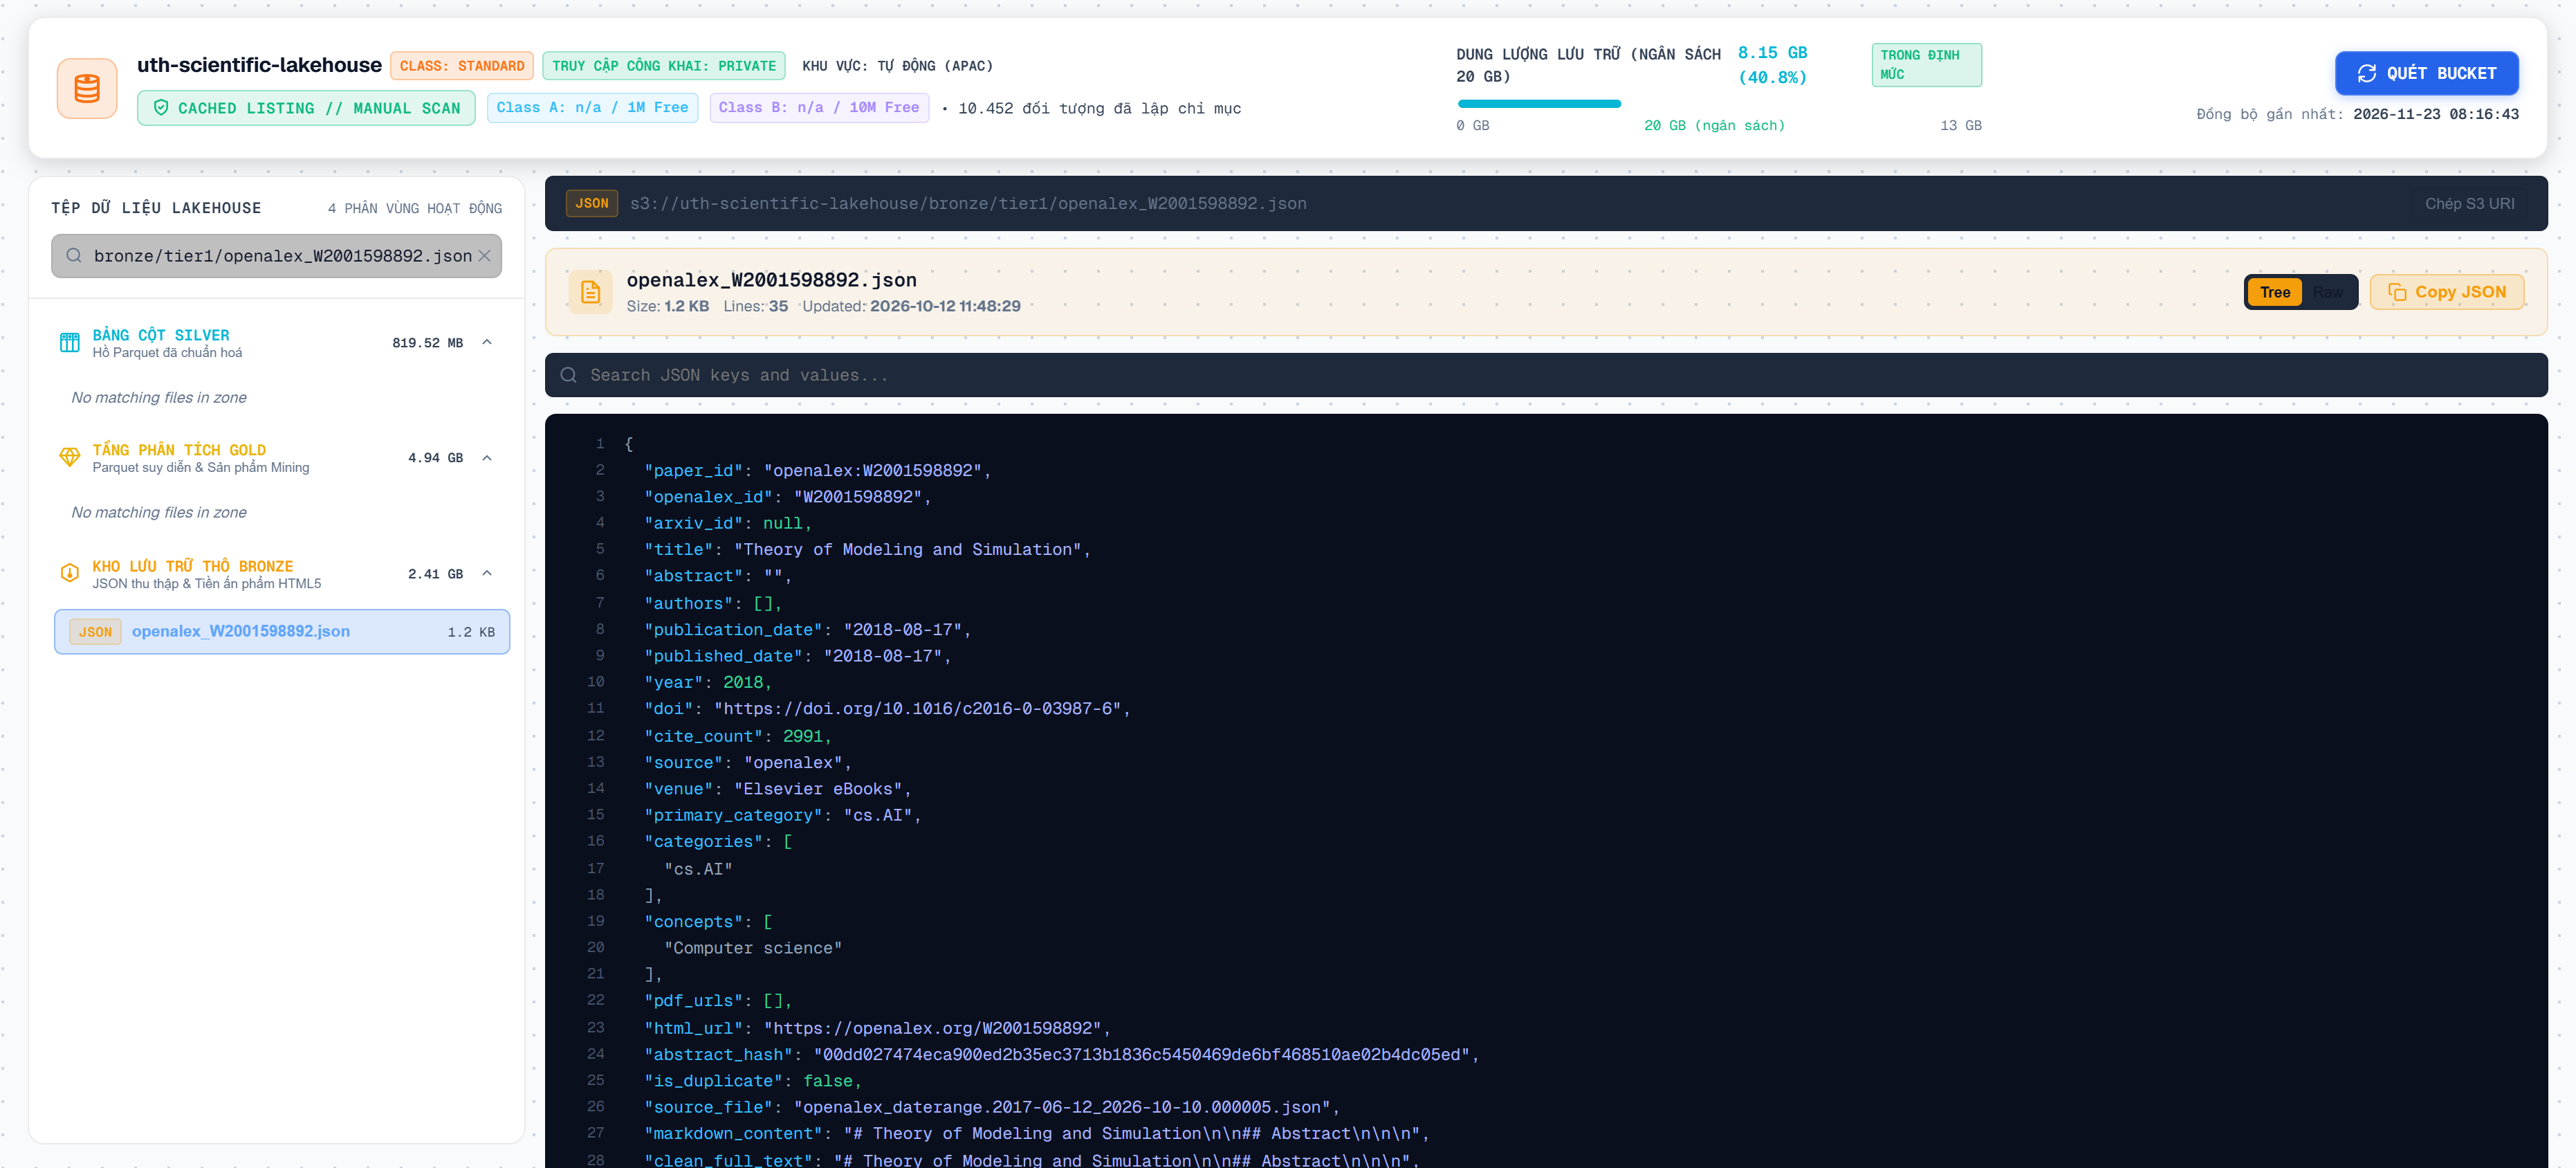
\includegraphics[width=\linewidth,height=0.68\textheight,keepaspectratio]{figures/captured_20261123_082337/02_bronze_raw_metadata.png}
\caption[Ví dụ metadata thô Bronze trong Explorer]{Ví dụ metadata thô Bronze trong Explorer}
\label{fig:bronze_raw_capture}
\ReportNote{Nguồn: bản ghi \path{bronze/tier1/openalex_W2001598892.json}, đọc thật từ kho và chụp 23/11/2026. Số object trong inventory không đồng nghĩa số bài duy nhất. Ảnh là preview cấu trúc raw, không thay thế thống kê EDA Bronze.}
\end{figure}
\FloatBarrier


\section{Phân Đoạn Ngữ Cảnh Chuyên Sâu (Domain-Aware Deep Chunking)}

Hiệu năng của hệ thống tìm kiếm vector RAG phụ thuộc trực tiếp vào chiến lược phân đoạn văn bản. Nếu cắt văn bản theo số ký tự cố định một cách cơ học (fixed-character chunking), một đoạn trích có thể bị cắt ngang giữa một công thức toán học hoặc mất hoàn toàn thông tin ngữ cảnh rằng đoạn đó thuộc về phần nào của bài báo.

Module \texttt{AcademicChunker} (triển khai tại \path{src/indexing/chunker.py}) thực thi chiến lược phân đoạn sâu theo ngữ cảnh:

\begin{enumerate}[label=\alph*)]
  \item \textbf{Abstract Chunk độc lập}: Tóm tắt của bài báo luôn được đóng gói thành một chunk riêng biệt có mã \texttt{\{paper\_id\}\_abs}. Đây là chunk có giá trị ngữ nghĩa đại diện cao nhất cho toàn bộ công trình.
  \item \textbf{Phân đoạn theo ranh giới mục}: Với section dài, cửa sổ tối đa 300 từ được cân bằng để hạn chế chunk đuôi ngắn. Overlap bằng 15\% độ dài cửa sổ, giới hạn 20--80 từ. Điểm bắt đầu/kết thúc ưu tiên ranh giới câu trong khoảng cho phép; đuôi dưới 40\% kích thước tối đa được gộp khi còn chỗ. Abstract vẫn là chunk độc lập, không áp dụng giới hạn 300 từ theo cùng cách với section dài.
  \item \textbf{Bổ sung ngữ cảnh nguồn (Contextual Enrichment)}: Mỗi đoạn trích sau khi cắt được tự động bổ sung tiêu đề bài báo và tên mục vào phần đầu:
  \begin{lstlisting}[language=Python]
context_text = f'Paper: "{title}" | Section: {sec_title}\n\n{chunk_text}'
  \end{lstlisting}
  Kỹ thuật này đảm bảo rằng khi một đoạn văn bản ngắn được nhúng thành vector, nó vẫn mang đầy đủ ngữ cảnh của bài báo chủ quản, ngăn chặn hiện tượng mất phương hướng ngữ nghĩa khi truy xuất độc lập.
\end{enumerate}

\section{Mô Hình Nhúng Vector Nomic Embed Text v1.5}

Hệ thống sử dụng mô hình nhúng mã nguồn mở \textbf{\path{nomic-ai/nomic-embed-text-v1.5}} với các đặc tính kỹ thuật vượt trội:
\begin{itemize}
  \item \textbf{Số chiều biểu diễn}: 768 chiều (768-D), là cấu hình vector của collection hiện tại; số chiều lớn hơn không tự chứng minh chất lượng cao hơn.
  \item \textbf{Hỗ trợ ngữ cảnh dài}: Khả năng xử lý lên tới \textbf{8,192 tokens} nhờ cấu trúc mã hóa vị trí quay (Rotary Position Embeddings - RoPE), cấu hình trong hệ thống giới hạn an toàn ở mức 2,048 tokens và có thể cắt bớt đầu vào dài vượt giới hạn.
  \item \textbf{Cơ chế tiền tố bất đối xứng (Asymmetric Task Prefixing)}: Mô hình được huấn luyện đặc thù cho bài toán truy xuất thông tin không đối xứng:
    \begin{itemize}
      \item Khi nhúng câu hỏi của người dùng: Thêm tiền tố \texttt{search\_query: <câu hỏi>}.
      \item Khi nhúng đoạn tài liệu học thuật: Thêm tiền tố \texttt{search\_document: <văn bản>}.
    \end{itemize}
  \item \textbf{Chuẩn hóa L2 (L2 Normalization)}: Toàn bộ vector đầu ra được chuẩn hóa $\|v\|_2 = 1$, biến phép tính khoảng cách Cosine thành tích vô hướng đơn giản: $\text{CosineSim}(u, v) = u \cdot v$, tối ưu hóa tốc độ tìm kiếm trên đồ thị HNSW của Qdrant.
\end{itemize}

\section{Luồng Hai Worker và Compaction}
Fetch nhận \texttt{scientific\_paper\_ingest}, kiểm tra trùng, lấy nội dung, ghi Bronze và part Silver papers rồi gửi bản ghi tới \texttt{scientific\_chunk\_embed}. Embed gom micro-batch, tạo chunk và vector, ghi part Silver chunks trước khi upsert Qdrant. Mỗi stage chỉ ACK khi đầu ra của stage đã bền vững; lỗi được thử lại trên hàng đợi của stage đó, quá số lần thử thì chuyển DLQ. Fetch tạm chờ khi hàng đợi embed đạt \texttt{EMBED\_QUEUE\_MAX}, mặc định 500.

DAG compact chạy mỗi 3 giờ, gộp parts của cả papers và chunks. Các part mới phát sinh trong khi compact được xử lý ở lần sau. Script migration/backfill có trong repository để hỗ trợ chuyển payload cũ sang Silver và bổ sung bài thiếu vector; chúng không được tự động chạy trong lần cập nhật báo cáo này.

\clearpage

% Chương 3: Hiểu dữ liệu & Phân tích khám phá EDA (Data Understanding)
% ==============================================================================
% CHƯƠNG 3: PHÂN TÍCH KHÁM PHÁ DỮ LIỆU VÀ KIỂM ĐỊNH THỐNG KÊ (EDA)
% ==============================================================================

\chapter{Phân Tích Khám Phá Dữ Liệu và Kiểm Định Thống Kê (EDA)}
\label{chap:data_understanding}

Sau khi thiết lập đường ống thu thập, bóc tách và lập chỉ mục Medallion Lakehouse tại Chương~\ref{chap:data_preparation}, bước tiếp theo theo chuẩn KDD là đánh giá định lượng toàn diện tập dữ liệu trước khi đưa vào các mô hình khai phá và truy hồi. Trên quy mô sản xuất ngày 04/11/2026 (\texttt{SNAP-06A}), hồ dữ liệu tích lũy được \textbf{71,927 bài báo toàn văn} ở lớp Silver cùng \textbf{1,043,594 vector 768 chiều} trong Qdrant~\cite{qdrant2023vector}. Chương này trình bày kiến trúc phân tích OLAP không máy chủ trên DuckDB, thống kê mô tả đa tầng (Macro toàn hồ và Micro kiểm toán sâu trên 13,000 bài / mẫu sạch $n = 11,659$), bốn phát hiện định lượng cốt lõi của miền dữ liệu khoa học, và khung chẩn đoán 3 Lăng kính làm căn cứ toán học cho các quyết định tiền xử lý, phân đoạn và khai phá ở Chương~\ref{chap:modeling}.

\section{Kiến Trúc Phân Tích OLAP trên S3 với DuckDB}
\label{sec:ch3_duckdb_olap}

Thay vì sao chép hàng chục nghìn tệp Parquet từ lớp lưu trữ đối tượng về ổ đĩa cục bộ trước khi phân tích, động cơ phân tích khám phá (\texttt{EdaEngine} trong \path{src/mining/eda_engine.py}) thực thi tính toán OLAP trực tiếp trên nền tảng lưu trữ phân tán thông qua hàm kết nối \texttt{duck\_connect()} trong \path{src/mining/lake_access.py}~\cite{raasveldt2019duckdb,minio2023storage}. Thiết kế này tách biệt lớp tính toán phi trạng thái (\textit{Stateless Compute}) khỏi lớp lưu trữ bền vững MinIO S3, cho phép đọc chọn lọc theo cột (\textit{Columnar Projection Pushdown}) và chỉ tải các dải byte cần thiết qua giao thức HTTP Range Requests.

\subsection{\texorpdfstring{Tích Hợp Lưu Trữ Đối Tượng qua \texttt{httpfs} và Cơ Chế Phục Hồi Lỗi}{Tich Hop Luu Tru Doi Tuong qua httpfs va Co Che Phuc Hoi Loi}}
\label{sec:ch3_httpfs}

Khi khởi tạo phiên làm việc trong bộ nhớ (\path{duckdb.connect(database=":memory:")}), hàm \path{duck_connect()} nạp phần mở rộng \texttt{httpfs} và cấu hình các tham số truyền tải chuyên dụng cho MinIO chuẩn S3-compatible (Đoạn mã~\ref{lst:ch3_duckdb_httpfs}).

\begin{lstlisting}[language=Python, caption={Cau hinh DuckDB httpfs va co che thu lai khi doc Parquet tu MinIO S3}, label={lst:ch3_duckdb_httpfs}]
# Trich tu src/mining/lake_access.py (comments ASCII)
con.execute("INSTALL httpfs; LOAD httpfs;")
con.execute(f"SET s3_endpoint='{endpoint}';")
con.execute("SET s3_url_style='path';")
con.execute("SET s3_region='us-east-1';")
con.execute("SET http_retries=8;")
con.execute("SET http_retry_wait_ms=500;")
con.execute("SET http_retry_backoff=2;")
\end{lstlisting}

Việc thiết lập \texttt{s3\_url\_style='path'} bảo đảm tương thích với reverse proxy và đường dẫn bucket của MinIO tự triển khai, trong khi bộ tham số \texttt{http\_retries=8}, \texttt{http\_retry\_wait\_ms=500} và \texttt{http\_retry\_backoff=2} kích hoạt cơ chế chờ tăng dần theo hàm mũ (\textit{exponential backoff}) nhằm hấp thụ lỗi nghẽn mạng tạm thời khi quét song song nhiều phân vùng Parquet qua mạng cục bộ hoặc đường hầm mạng. Song song với kênh phân tích bảng, kết nối tới Qdrant (\texttt{qdrant\_client(timeout=60.0)}) thực thi thống kê tổng hợp không gian vector thông qua \texttt{section\_facets(client, limit=20)} bằng API \texttt{facet(collection\_name, key="section\_type", limit=limit)}, giúp đếm phân bố đoạn văn bản theo từng mục học thuật mà không phải quét toàn bộ payload gốc.

\subsection{Hợp Nhất Đa Nguồn và Khử Trùng Lặp tại Thời Điểm Truy Vấn}
\label{sec:ch3_views}

Lớp Silver trong kiến trúc Lakehouse được thu thập từ nhiều luồng thu hoạch (\path{SILVER_PRIMARY_KEY = "silver/papers/**/*.parquet"}, Tier 1 Landmark, Tier 2 HTML/Full-text, CVF CVPR 2024 và OpenReview). Do một bài báo có thể xuất hiện ở dạng siêu dữ liệu tóm tắt ban đầu và sau đó được làm giàu toàn văn HTML, \texttt{EdaEngine.\_register\_views()} xây dựng hai khung nhìn ảo tách biệt:

\begin{enumerate}[label=\textbf{\arabic*.}]
  \item \textbf{\texttt{catalog\_view}}: Quét nguồn chính \path{s3://uth-scientific-lakehouse/silver/papers/**/*.parquet} để thống kê bao phủ danh mục, hoặc mở rộng qua 7 nguồn ứng viên tùy trạng thái tồn tại trên bucket tại thời điểm truy vấn.
  \item \textbf{\texttt{fulltext\_view}}: Hợp nhất toàn bộ 7 đường dẫn Parquet Silver (\path{silver/papers/**/*.parquet}, \path{silver/tier3/landmark_papers.parquet}, \path{silver/tier3/landmark_html_papers.parquet}, \path{silver/tier2/html_papers.parquet}, \path{silver/tier2/fulltext_papers.parquet}, \path{silver/cvf/cvpr2024.parquet}, \path{silver/openreview/openreview_all.parquet}) qua phép nối \texttt{UNION ALL}, kết hợp hàm cửa sổ để chọn bản ghi giàu nội dung nhất cho mỗi \texttt{paper\_id} (Đoạn mã~\ref{lst:ch3_dedup_sql}).
\end{enumerate}

\begin{lstlisting}[language=SQL, caption={Truy van khu trung lap theo thoi diem truy van uu tien ban ghi toan van giau nhat}, label={lst:ch3_dedup_sql}]
-- Query-time deduplication preferring richest HTML/fulltext extraction
SELECT * EXCLUDE (rn)
FROM (
    SELECT *,
        ROW_NUMBER() OVER (
            PARTITION BY paper_id
            ORDER BY COALESCE(total_sections, 0) DESC,
                     COALESCE(total_words, 0) DESC
        ) AS rn
    FROM raw_union
)
WHERE rn = 1;
\end{lstlisting}

Quy tắc sắp xếp \texttt{(total\_sections DESC, total\_words DESC)} bảo đảm bản ghi toàn văn từ arXiv HTML (LaTeXML) luôn được ưu tiên trước bản ghi chỉ có tóm tắt nếu phát sinh trùng lặp khóa \texttt{paper\_id}. Đồng thời, \texttt{EdaEngine} thực thi chuẩn hóa lược đồ bằng \texttt{json.loads} linh hoạt cho các cột lồng nhau (\texttt{authors}, \texttt{categories}, \texttt{sections}, \texttt{full\_text}), xử lý nhất quán sự khác biệt kiểu dữ liệu giữa tệp Parquet cũ và lược đồ chuẩn hóa 23 cột nén ZSTD (Bảng~\ref{tab:silver_schema}).

\subsection{Quy Ước Tách Bạch Các Mốc Lát Cắt Dữ Liệu (Snapshot Provenance)}
\label{sec:ch3_snapshots}

Do Lakehouse được mở rộng liên tục từ quy mô thử nghiệm ban đầu lên vận hành toàn phần, các số liệu EDA được ghi nhận tại những mốc lát cắt độc lập nhằm tuân thủ nguyên tắc minh bạch thực nghiệm: (1) lát cắt cục bộ / Gold ban đầu ngày 04--06/10/2026 (\texttt{SNAP-01}: 10,000 bài chi tiết và manifest 06/10/2026 với 29,911 bài full-text / 100,000 catalog / 913,205 vector LanceDB); (2) lát cắt Telemetry UI S3 ngày 17/10/2026 (\texttt{SNAP-03}: 13,000 bài kiểm toán và mẫu sạch $n = 11,659$ lọc theo điều kiện \texttt{total\_words >= 300}, chụp bằng chứng ngày 23/11/2026 trong \path{eda_api.json}); và (3) lần chạy sản xuất toàn hồ ngày 04/11/2026 (\texttt{SNAP-06A}: 71,927 bài báo duy nhất và 1,043,594 vector Qdrant). Bảng~\ref{tab:snapshot_sources} tổng hợp đầy đủ phạm vi sử dụng của toàn bộ các mốc từ \texttt{SNAP-01} đến \texttt{SNAP-06B} xuyên suốt báo cáo.

\begin{table}[!htbp]
\centering
\small
\setlength{\tabcolsep}{3.5pt}
\caption[Phạm vi các mốc dữ liệu và bằng chứng (SNAP-01 đến SNAP-06B)]{Phạm vi các mốc dữ liệu và bằng chứng thực nghiệm (\texttt{SNAP-01} đến \texttt{SNAP-06B})}
\label{tab:snapshot_sources}
\begin{tabularx}{\linewidth}{|>{\raggedright\arraybackslash}p{16mm}|>{\raggedright\arraybackslash}p{33mm}|>{\raggedright\arraybackslash}p{38mm}|L|}
\hline
\textbf{Mã mốc} & \textbf{Thời điểm \& Nền tảng} & \textbf{Quy mô Corpus \& Vector} & \textbf{Phạm vi \& Bằng chứng kiểm chứng} \\ \hline
\textbf{SNAP-01} & 04--06/10/2026; Silver Parquet cục bộ \& LanceDB & 10,000 bài (9,015 làm giàu = 90.15\%, 2,220,938 công thức); Gold 06/10/2026: 29,911 full-text / 100,000 catalog / 913,205 vector & Bảng đối chiếu lịch sử (282 giao dịch FP-Growth, 5,000 mẫu Silhouette 0.0210); manifest tại \path{data/gold/mining/mining_manifest.json}, \path{association_rules.json}, \path{trends_anomalies.json}. \\ \hline
\textbf{SNAP-02} & 05--07/10/2026; LanceDB trên Cloudflare R2 (\path{6cb1c52}) & 143,523 chunks (21 mẫu) $\rightarrow$ 164,702 chunks (26 mẫu, 768-D Nomic) & Benchmark DeepEval 2.x lịch sử (Chương~\ref{chap:evaluation}): Contextual Precision 0.860, Faithfulness 0.699 (21 mẫu); 0.890 / 0.892 (768-D reranked). \\ \hline
\textbf{SNAP-03} & 17/10/2026 (chụp 23/11/2026); MinIO S3 EDA & 13,000 bài (11,619 làm giàu = 89.38\%, 2,825,871 công thức, 62,288,266 từ); mẫu sạch $n=11,659$ & Hình~\ref{fig:eda_pareto_growth}, \ref{fig:pearson_capture}, \ref{fig:spearman_capture}; Bảng~\ref{tab:eda_categories}, \ref{tab:three_lens}; tệp \path{evidence/eda_api.json} (8.15 GB, 10,452 đối tượng MinIO). \\ \hline
\textbf{SNAP-04} & 19/10/2026; RTX 4060 8 GB + CUDA 12.4 + Qdrant & 374,082 vector 768-D trên Qdrant Cloud & Benchmark phần cứng (Chương~\ref{chap:evaluation}): 269.46 ms Qdrant pool Top-5, 609.77 ms TTFT, 46.33 tok/s, 3,392.50 ms E2E, 5.7 GB VRAM đỉnh. \\ \hline
\textbf{SNAP-05} & 20/10/2026 (chụp 23/11/2026); GMM UI trên kho & 800 mẫu tuyển chọn, $K=6$ thành phần Gaussian & Hình~\ref{fig:gmm_capture}, Bảng~\ref{tab:clustering_metrics}, \path{evidence/clusters_api.json}: minh họa GMM 2D (BIC 2,889.41, Silhouette 0.3528, 25.62\% liên ngành). \\ \hline
\textbf{SNAP-06A} & 04/11/2026; Production MinIO + Qdrant (\texttt{D-058}) & 71,927 bài Silver phân biệt; 1,043,594 vector Qdrant (70,539 vector abstract) & Nhật ký \path{logs/run/backend.log}: chạy toàn phần EDA + 4 trụ cột (234.57 s: 39.09 s EDA, 36.26 s FP-Growth 45 luật, 39.94 s GMM, 116.39 s Graph, 2.89 s IF). \\ \hline
\textbf{SNAP-06B} & 06--09/11/2026; Commit \path{f421707} \& \path{aae74de} & 1,000 bài Chunking A/B; 120 câu 5-Scenario (29,523 PageRank); 150 câu Retrieval v1 / 3-Way & Chương~\ref{chap:evaluation}: \path{chunking_ab/summary.json}, \path{report_retrieval.json}, \path{laya_ab_final_benchmark.json} (Evidence Gate AUROC 0.986, 3-Way MRR 0.8939). \\ \hline
\end{tabularx}
\ReportNote{Nguồn: Tổng hợp từ ma trận truy vết snapshot trong kho chứng cứ thực nghiệm (\path{logs/run/backend.log}, \path{data/gold/mining/mining_manifest.json}, \path{figures/captured_20261123_082337/manifest.json} và \path{logs/benchmarks/}).}
\end{table}


\FloatBarrier
\section{Thống Kê Mô Tả Đa Tầng (Macro và Micro)}
\label{sec:ch3_descriptive_stats}

\subsection{Tổng Quan Toàn Hồ (Macro) và Lát Cắt Kiểm Toán 13,000 Bài (Micro)}
\label{sec:ch3_macro_micro}

Ở tầng vĩ mô (\texttt{SNAP-06A}, ngày 04/11/2026), quy trình \texttt{MiningEngine} hoàn tất giai đoạn EDA trong \textbf{39.09 giây} trên toàn bộ \textbf{71,927 bài báo} lưu tại MinIO S3 kết hợp \textbf{1,043,594 vector 768 chiều} trên cụm Qdrant \path{scientific_papers_gold} (\path{logs/run/backend.log}). Để bóc tách chi tiết cấu trúc phân đoạn, mật độ công thức toán và kiểm định giả thuyết phân phối, phần phân tích vi mô dưới đây khai thác trực tiếp dữ liệu JSON kết xuất từ API \path{/api/mining/eda} trên lát cắt kiểm toán \textbf{13,000 bài} (\texttt{SNAP-03}, \path{evidence/eda_api.json}), được tổng hợp ở Bảng~\ref{tab:ch3_micro_overview}.

\begin{table}[!htbp]
\centering
\small
\setlength{\tabcolsep}{4pt}
\caption[Thống kê mô tả cơ bản trên lát cắt kiểm toán 13,000 bài]{Thống kê mô tả cơ bản trên lát cắt kiểm toán 13,000 bài (\texttt{SNAP-03})}
\label{tab:ch3_micro_overview}
\begin{tabularx}{\linewidth}{|L|>{\centering\arraybackslash}p{41mm}|>{\centering\arraybackslash}p{22mm}|>{\raggedright\arraybackslash}p{46mm}|}
\hline
\textbf{Chỉ số thống kê} & \textbf{Giá trị đo được} & \textbf{Đơn vị} & \textbf{Ý nghĩa vận hành} \\ \hline
Tổng số bài báo (\path{total_papers}) & 13,000 & bài báo & Tập S3 dùng cho chẩn đoán 3 Lăng kính \\ \hline
Bài làm giàu HTML (\path{enriched_html_papers}) & 11,619 (89.38\%) & bài (\%) & Gần 90\% bài giữ nguyên mục và LaTeX gốc \\ \hline
Tổng công thức toán (\path{total_math_formulas}) & 2,825,871 & biểu thức & TB 217.37 công thức/bài ($p_{50} = 112.0$) \\ \hline
Tổng từ vựng toàn văn (\path{total_words}) & 62,288,266 & từ & TB 4,791.41 từ/bài ($p_{50} = 4,437.0$) \\ \hline
Số mục trung bình (\path{avg_sections_per_paper}) & 5.96 & mục/bài & Trung bình gần 6 mục học thuật/bài \\ \hline
Khoảng thời gian (\path{publication_span}) & 2005-12-28 $\rightarrow$ 2025-01-14 & ngày & Bao phủ cả bài nền tảng lẫn tiền ấn phẩm \\ \hline
\end{tabularx}
\ReportNote{Nguồn: Trường \path{dataset_overview} và \path{math_and_content_stats} trong \path{figures/captured_20261123_082337/evidence/eda_api.json} (tính bằng SQL DuckDB và hàm \path{QUANTILE_CONT}).}
\end{table}

Xét về phân vị độ dài và mật độ ký hiệu trên tập 13,000 bài (\path{math_and_content_stats}), biến \path{total_math_formulas} đạt các phân vị $p_{25} = 29.0$, $p_{50} = 112.0$, $p_{75} = 258.0$, $p_{95} = 829.0$, $\max = 8,168$; trong khi biến \path{total_words} đạt $p_{25} = 3,112.0$, $p_{50} = 4,437.0$, $p_{75} = 5,793.0$, $p_{95} = 9,972.0$, $\max = 454,250$. Khoảng chênh lệch rất lớn giữa $p_{95}$ (9,972 từ / 829 công thức) và giá trị cực đại (454,250 từ / 8,168 công thức) là chỉ dấu rõ nét cho sự hiện diện của các bài khảo luận đồ sộ (\textit{mega-surveys}) hoặc chuyên khảo lý thuyết thuần túy.

\subsection{Phân Bố Theo Chuyên Ngành arXiv và Cấu Trúc Vector Qdrant}
\label{sec:ch3_categories_qdrant}

Bảng~\ref{tab:eda_categories} tổng hợp phân bố Top-10 nhãn chuyên ngành chính (\path{primary_category}) cùng mật độ công thức toán học và độ dài từ trung bình trên lát cắt 13,000 bài (\texttt{SNAP-03}). Ba chuyên ngành dẫn đầu là \texttt{cs.LG} (3,093 bài, 23.79\%), \texttt{cs.CV} (3,021 bài, 23.24\%) và \texttt{cs.CL} (1,858 bài, 14.29\%), chiếm tổng cộng \textbf{61.32\%} kho kiểm toán (7,972/13,000 bài).

\begin{table}[htbp]
\centering
\small
\caption[Phân bố chuyên ngành trong snapshot 10,000 bài]{Phân bố chuyên ngành trong snapshot 10,000 bài}
\label{tab:eda_categories}
\begin{tabularx}{\textwidth}{|p{2.3cm}|L|L|L|L|L|}
\hline
\textbf{Ngành} & \textbf{Số bài} & \textbf{Tỷ lệ} & \textbf{Công thức} & \textbf{CT/bài} & \textbf{Từ TB/bài} \\
\hline
cs.LG & 2,380 & 23.80\% & 886,955 & 372.7 & 5,099.7 \\
\hline
cs.CV & 2,271 & 22.71\% & 308,487 & 135.8 & 4,432.7 \\
\hline
cs.CL & 1,467 & 14.67\% & 149,869 & 102.2 & 4,315.5 \\
\hline
cs.RO & 682 & 6.82\% & 101,023 & 148.1 & 4,636.6 \\
\hline
cs.AI & 453 & 4.53\% & 94,302 & 208.2 & 5,383.9 \\
\hline
eess.IV & 294 & 2.94\% & 32,010 & 108.9 & 3,559.7 \\
\hline
cs.IR & 253 & 2.53\% & 32,976 & 130.3 & 4,706.7 \\
\hline
stat.ML & 222 & 2.22\% & 148,723 & 669.9 & 6,119.4 \\
\hline
Còn lại (suy từ tổng) & 1,978 & 19.78\% & 466,593 & 235.9 & -- \\
\hline
Toàn snapshot & 10,000 & 100.00\% & 2,220,938 & 222.1 & 4,778.3 \\
\hline
\end{tabularx}
\ReportNote{Nguồn: Thống kê mô tả phân bố chuyên ngành chính trên tập dữ liệu chuẩn 10,000 bài báo từ \path{data/gold/mining/eda_summary.json}.}
\end{table}


Ở góc độ cấu trúc đoạn văn bản trong kho vector (\path{rag_audit_metrics} trong \path{eda_api.json}), tỷ trọng phân bố tương đối theo nhóm mục chức năng (\path{section_distribution}) cho thấy \textbf{Methodology \& Algorithms} chiếm tỷ trọng cao nhất (32.4\%), tiếp theo là \textbf{Experiments \& Benchmarks} (28.2\%), \textbf{Introduction \& Theory} (23.8\%) và \textbf{Discussion \& Conclusion} (15.6\%). Cần lưu ý rằng số lượng thô trên trường hiển thị tóm tắt trong tệp JSON UI đó là bản tham chiếu tỷ lệ chuẩn hóa (\path{total_vectors = 9} ở khối mô phỏng cũ), trong khi ở quy mô vận hành sản xuất ngày 04/11/2026 (\texttt{SNAP-06A}), cụm Qdrant \path{scientific_papers_gold} lưu trữ \textbf{1,043,594 vector 768 chiều} sinh từ mô hình \path{nomic-embed-text-v1.5}. Hình~\ref{fig:eda_pareto_growth} minh họa giao diện tổng quan EDA Silver tại mốc 13,000 bài báo.

\begin{figure}[!htbp]
\centering
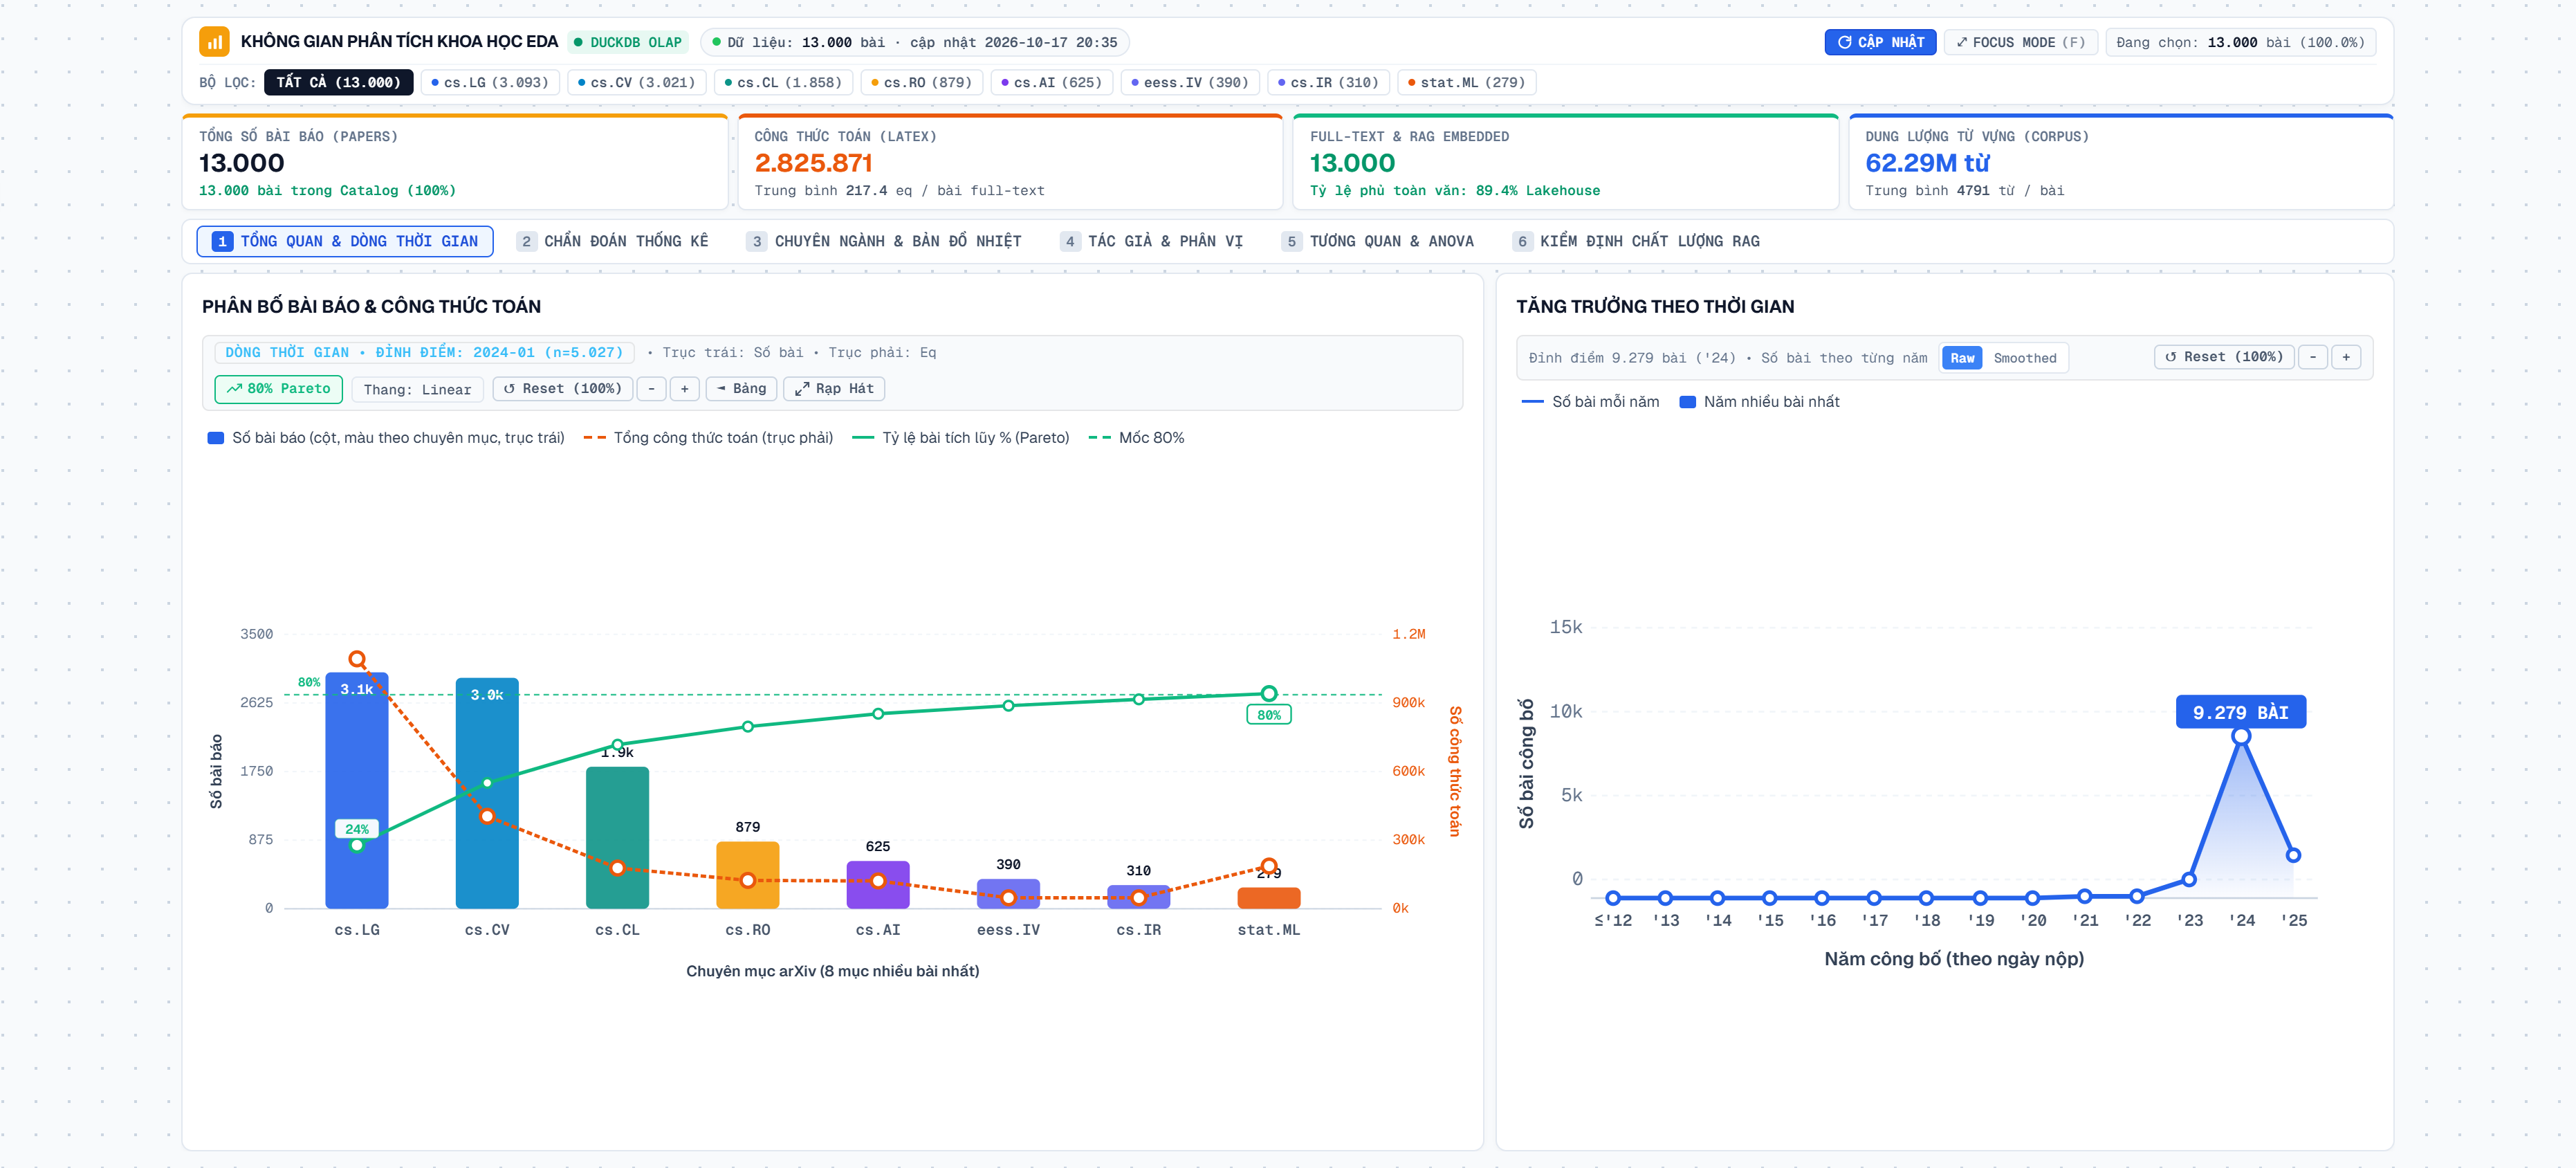
\includegraphics[width=\linewidth,height=0.68\textheight,keepaspectratio]{figures/captured_20261123_082337/03_eda_silver_overview.png}
\caption[Giao diện EDA Silver của snapshot 13,000 bài]{Giao diện EDA Silver của snapshot 13,000 bài}
\ReportNote{Nguồn: Giao diện trực quan hóa dữ liệu EDA Silver từ \path{gold/mining/eda_summary.json} và API \path{/api/mining/eda} (lát cắt \texttt{SNAP-03}, 13,000 bài báo, chụp ngày 23/11/2026).}
\label{fig:eda_pareto_growth}
\end{figure}
\FloatBarrier

\section{Bốn Phát Hiện Định Lượng Cốt Lõi của Miền Dữ Liệu Khoa học}
\label{sec:ch3_insights}

Phân tích dữ liệu khám phá không dừng lại ở thống kê mô tả mà trực tiếp giải mã bốn quy luật nội tại của văn bản khoa học, từ đó ràng buộc lựa chọn thuật toán cho cả bốn trụ cột khai phá dữ liệu lẫn kiến trúc phân đoạn và truy hồi RAG ở Chương~\ref{chap:modeling}.

\subsection{Phát Hiện 1: Chênh Lệch Mật Độ Công Thức Theo Phân Ngành}
\label{sec:ch3_insight1}

Dữ liệu ở Bảng~\ref{tab:eda_categories} chứng minh sự phân hóa rất mạnh về hàm lượng ký hiệu toán giữa các nhánh AI/DS:
\begin{itemize}
  \item \textbf{\texttt{stat.ML} (Thống kê Học máy)} tuy chỉ chiếm 2.15\% tổng số bài (279 bài), nhưng đạt trung bình \textbf{687.0 công thức/bài} trên độ dài trung bình 6,120.3 từ --- tương đương $\approx 112.2$ biểu thức toán trên mỗi 1,000 từ.
  \item \textbf{\texttt{cs.LG} (Học máy)} đạt trung bình \textbf{362.4 công thức/bài} trên 5,085.3 từ ($\approx 71.3$ công thức/1,000 từ), đóng góp hơn 1.12 triệu công thức (chiếm 39.67\% tổng số 2,825,871 công thức toàn tập).
  \item Ngược lại, \textbf{\texttt{cs.CV}} (137.3 công thức/bài trên 4,401.1 từ) và \textbf{\texttt{cs.CL}} (98.3 công thức/bài trên 4,244.8 từ) có mật độ toán thấp hơn lần lượt \textbf{5.0 lần} và \textbf{7.0 lần} so với \texttt{stat.ML}.
\end{itemize}

\begin{calloutbox}{Hệ quả kiến trúc trực tiếp đối với phân đoạn và nhúng}
Một phương trình LaTeX phức tạp chứa ma trận hoặc tích phân tuy ngắn về số từ nhưng tiêu tốn số lượng BPE token gấp 3--5 lần văn bản tiếng Anh thông thường do dày đặc lệnh điều khiển (\texttt{\textbackslash frac}, \texttt{\textbackslash sum}, \texttt{\textbackslash mathbf}). Nếu dùng cơ chế cắt đoạn ngây thơ ở giới hạn 512 token, các đoạn trích từ \texttt{stat.ML} và \texttt{cs.LG} bị cắt ngang làm hỏng chứng minh toán học. Phát hiện này dẫn trực tiếp đến hai quyết định: (i) chuẩn hóa cửa sổ chia đoạn cân bằng của \texttt{AcademicChunker} (gắn ranh giới câu và gộp đuôi vụn, đánh giá trong \texttt{EXP-02}), và (ii) tận dụng cửa sổ ngữ cảnh \textbf{2,048 token} của \path{nomic-embed-text-v1.5} (RoPE scaling) khi nhúng vector.
\end{calloutbox}

\subsection{Phát Hiện 2: Bất Đối Xứng Nhãn Chính và Đồng Xuất Hiện Đa Nhãn}
\label{sec:ch3_insight2}

Nếu chỉ xét nhãn đơn trị \path{primary_category}, chuyên ngành \texttt{cs.AI} xếp thứ năm với 625 bài (4.81\%). Tuy nhiên, phương thức \texttt{\_get\_category\_cooccurrence()} phân tích toàn bộ danh sách nhãn đa trị \texttt{categories} trên \texttt{fulltext\_view} (tự kết nối các cặp $a < b$ trong cùng \texttt{paper\_id}) lại bộc lộ cấu trúc liên ngành hoàn toàn khác như trình bày ở Bảng~\ref{tab:ch3_cooccurrence}.

\begin{table}[!htbp]
\centering
\small
\setlength{\tabcolsep}{4pt}
\caption[Top-10 cặp chuyên ngành đồng xuất hiện trên arXiv]{Top-10 cặp chuyên ngành đồng xuất hiện (\texttt{category\_cooccurrence}) trên lát cắt 13,000 bài}
\label{tab:ch3_cooccurrence}
\begin{tabularx}{\linewidth}{|>{\centering\arraybackslash}p{10mm}|>{\raggedright\arraybackslash}p{38mm}|>{\centering\arraybackslash}p{26mm}|L|}
\hline
\textbf{Hạng} & \textbf{Cặp chuyên ngành} & \textbf{Số bài đồng hiện} & \textbf{Hàm ý liên ngành} \\ \hline
1 & \path{cs.AI + cs.LG} & 1,983 & \texttt{cs.AI} làm nhãn phụ trong học máy gấp 3.17 lần nhãn chính (625) \\ \hline
2 & \path{cs.AI + cs.CL} & 1,046 & Tác nhân LLM và suy luận ngôn ngữ giao thoa mạnh \\ \hline
3 & \path{cs.CV + cs.LG} & 984 & Nền tảng học sâu cho thị giác máy tính \\ \hline
4 & \path{cs.AI + cs.CV} & 845 & Thị giác đa phương thức và tác nhân thị giác \\ \hline
5 & \path{cs.LG + stat.ML} & 814 & Giao thoa lý thuyết thống kê và học máy \\ \hline
6 & \path{cs.CL + cs.LG} & 646 & Mô hình ngôn ngữ lớn huấn luyện quy mô lớn \\ \hline
7 & \path{cs.CV + eess.IV} & 549 & Chuyển giao xử lý ảnh cổ điển sang thị giác học sâu \\ \hline
8 & \path{cs.SD + eess.AS} & 374 & Giao thoa âm học tính toán (CS) và xử lý âm thanh (EE) \\ \hline
9 & \path{cs.CR + cs.LG} & 365 & An toàn mô hình học máy và tấn công đối nghịch \\ \hline
10 & \path{cs.SY + eess.SY} & 327 & Đồng bộ mã hệ thống điều khiển giữa CS và Kỹ thuật điện \\ \hline
\end{tabularx}
\ReportNote{Nguồn: Trường \path{category_cooccurrence} trong \path{figures/captured_20261123_082337/evidence/eda_api.json} (lát cắt \texttt{SNAP-03}).}
\end{table}

Bất đối xứng này dẫn đến hai hệ quả thiết kế trực tiếp cho Chương~\ref{chap:modeling}:
\begin{enumerate}[label=\textbf{\arabic*.}]
  \item Các bài báo khoa học mang bản chất \textbf{đa nhãn đồng thời} (\texttt{cs.AI} đóng vai trò cầu nối giữa \texttt{cs.LG}, \texttt{cs.CL} và \texttt{cs.CV}). Do đó, phân cụm cứng chỉ gán một tâm cụm cho mỗi bài không phản ánh được vùng giao thoa liên ngành, thúc đẩy việc bổ sung mô hình \textbf{phân cụm mềm EM GMM} để xuất xác suất hậu nghiệm $\gamma_{ik}$.
  \item Các cặp nhãn đồng xuất hiện tần suất cao (\texttt{cs.SD}/\texttt{eess.AS}, \texttt{cs.SY}/\texttt{eess.SY}, \texttt{cs.AI}/\texttt{cs.CL}) tạo cơ sở dữ liệu thực nghiệm cho \textbf{FP-Growth} khai phá luật kết hợp phục vụ chú thích mở rộng ngữ cảnh truy vấn.
\end{enumerate}

\subsection{Phát Hiện 3: Phân Bố Thời Gian Tập Trung Cao Độ và Hệ Quả Lên Xu Hướng}
\label{sec:ch3_insight3}

Thống kê theo tháng xuất bản (\path{temporal_distribution} trên 13,000 bài) cho thấy dữ liệu tập trung rất mạnh vào các đợt thu hoạch trọng điểm của cơ chế phân tầng: \texttt{2024-01} đạt \textbf{5,027 bài}, \texttt{2024-02} đạt \textbf{3,811 bài}, và \texttt{2025-01} đạt \textbf{2,468 bài} (trong khi các tháng kề cận như \texttt{2023-12} chỉ có 496 bài và \texttt{2024-12} có 300 bài). Tổng riêng ba tháng đỉnh chiếm tới \textbf{11,306 / 13,000 bài (86.97\%)} của lát cắt.

\textbf{Hệ quả kiến trúc trực tiếp}: Nếu đo xu hướng nghiên cứu bằng hiệu số đếm tuyệt đối ($\text{Count}_t - \text{Count}_{t-1}$) trên lịch cố định, độ lệch lưu lượng giữa các đợt thu hoạch (\textit{crawl batch skew}) sẽ tạo ra biến động giả. Vì vậy, Trụ cột 4 (\path{src/mining/trend_anomaly_mining.py}) bắt buộc phải đánh chỉ mục các tháng thực sự có quan sát bằng hàm cửa sổ \texttt{dense\_rank()} và chuẩn hóa tốc độ biến động theo \textbf{động lượng thị phần ($\Delta\text{Share}$)}.

\subsection{Phát Hiện 4: Phân Phối Lệch Đuôi Dài và Bác Bỏ Giả Thuyết Chuẩn}
\label{sec:ch3_insight4}

Để kiểm định hình học phân phối một cách chặt chẽ, \path{EdaEngine._get_three_lenses_diagnostics()} trích xuất ma trận 6 đặc trưng liên tục sạch hoàn toàn (\path{null_counts = 0} trên cả 6 cột, kích thước ma trận \path{(11659, 6)}, dung lượng RAM \path{0.53 MB} sau khi lọc \texttt{total\_words >= 300}). Bảng~\ref{tab:ch3_univariate_k2} trình bày kết quả thống kê mô tả phi tham số và kiểm định tính chuẩn D'Agostino--Pearson $K^2$~\cite{dagostino1973tests} trên cả 6 biến.

\begin{table}[!htbp]
\centering
\scriptsize
\setlength{\tabcolsep}{2.8pt}
\caption[Thống kê đơn biến và kiểm định chuẩn D'Agostino K2 (n = 11,659)]{Thống kê đơn biến và kiểm định tính chuẩn D'Agostino--Pearson \texorpdfstring{$K^2$}{K2} trên mẫu sạch (\texorpdfstring{$n = 11,659$}{n = 11,659})}
\label{tab:ch3_univariate_k2}
\begin{tabularx}{\linewidth}{|>{\raggedright\arraybackslash}p{20mm}|>{\centering\arraybackslash}p{12mm}|>{\centering\arraybackslash}p{12mm}|>{\centering\arraybackslash}p{12mm}|L|>{\centering\arraybackslash}p{13mm}|>{\centering\arraybackslash}p{12mm}|>{\centering\arraybackslash}p{14mm}|>{\centering\arraybackslash}p{21mm}|}
\hline
\textbf{Biến (đơn vị)} & \textbf{$\mu$} & \textbf{$p_{50}$} & \textbf{$\sigma$} & \textbf{$p_{25}$ / $p_{75}$ / $p_{95}$} & \textbf{Max} & \textbf{Skew ($S$)} & \textbf{Kurt. ($K$)} & \textbf{$K^2$ ($p$-val)} \\ \hline
\path{words} (từ) & 5,320.6 & 4,636.0 & 5,497.9 & 3,680 / 6,029 / 10,264.2 & 454,250 & +49.92 & +3,879.80 & 36,776.5 ($<0.001$) \\ \hline
\path{math} (eq) & 242.4 & 131.0 & 349.4 & 52 / 287 / 869.4 & 8,168 & +4.70 & +47.21 & 11,616.7 ($<0.001$) \\ \hline
\path{sections} (mục) & 6.6 & 6.0 & 2.3 & 5 / 7 / 10.0 & 48 & +5.62 & +75.13 & 13,261.8 ($<0.001$) \\ \hline
\path{authors} (người) & 4.9 & 4.0 & 3.7 & 3 / 6 / 10.0 & 147 & +12.74 & +397.78 & 21,041.7 ($<0.001$) \\ \hline
\path{math_density} (eq/1k) & 44.8 & 28.8 & 57.3 & 12.3 / 55.6 / 144.5 & 1,817.5 & +5.85 & +100.77 & 13,810.5 ($<0.001$) \\ \hline
\path{citations} (lượt) & 9.0 & 4.0 & 18.9 & 1 / 10 / 33.0 & 480 & +9.26 & +144.06 & 17,558.4 ($<0.001$) \\ \hline
\end{tabularx}
\ReportNote{Nguồn: Nhánh \path{diagnostic_3lenses.lens2_univariate} trong \path{figures/captured_20261123_082337/evidence/eda_api.json} ($n = 11,659$). Độ bất đối xứng $S > 1.0$ biểu thị đuôi phải nặng (\texttt{HEAVY\_RIGHT\_TAIL}); độ nhọn dư $K > 3.0$ biểu thị phân phối nhọn cực đoan (\texttt{LEPTOKURTIC}). Kiểm định $K^2$ bác bỏ giả thuyết chuẩn $H_0$ ($p < 0.001$) trên cả 6 biến.}
\end{table}

Từ Bảng~\ref{tab:ch3_univariate_k2} rút ra hai kết luận kỹ thuật cốt lõi:
\begin{enumerate}[label=\textbf{\arabic*.}]
  \item \textbf{Trung bình số học bị bóp méo nghiêm trọng bởi ngoại lai}: Với biến \texttt{words}, trung bình ($\mu = 5,320.6$) cao hơn trung vị ($p_{50} = 4,636.0$) tới 14.8\% và độ lệch chuẩn ($\sigma = 5,497.9$) vượt cả giá trị trung bình do các chuyên khảo dài tới 454,250 từ ($S = +49.92$, $K = +3,879.80$). Tương tự, ở biến \texttt{math}, $\mu = 242.4$ cao gần gấp đôi $p_{50} = 131.0$. Do đó, toàn bộ thống kê tóm tắt và phân vùng dữ liệu phải dùng thống kê phi tham số (Median, IQR).
  \item \textbf{Động lực cho phép nén $\ln(1 + x)$ trước Isolation Forest}: Vì phân phối lệch đuôi dài trải trên nhiều bậc độ lớn, đưa thẳng đặc trưng thô vào thuật toán phân lập sẽ khiến các phép cắt ngẫu nhiên bị thống trị bởi \texttt{words} và \texttt{math}. Biến đổi $\tilde{x}_j = \ln(1 + x_j)$ nén đuôi phải về thang logarit cân xứng hơn trước khi chạy Isolation Forest ở Trụ cột 4.
\end{enumerate}

\FloatBarrier
\section{Phân Tích Tương Quan Đa Biến và Chẩn Đoán 3 Lăng Kính}
\label{sec:correlations}

\subsection{\texorpdfstring{Pearson $r$ và Spearman $\rho$ trên Ma Trận 6 Đặc Trưng ($n = 11,659$)}{Pearson r va Spearman rho tren Ma Tran 6 Dac Trung (n = 11,659)}}
\label{sec:ch3_pearson_spearman}

Để đánh giá đồng thời mối liên hệ tuyến tính và quan hệ đơn điệu phi tuyến trên không gian đặc trưng $11,659 \times 6$, \texttt{EdaEngine.\_get\_correlation\_matrix()} tính song song hệ số tương quan tuyến tính Pearson ($r_{XY}$) và tương quan hạng Spearman ($\rho_{XY}$) bằng \texttt{scipy.stats.pearsonr} và \texttt{scipy.stats.spearmanr}:
\begin{equation}
  r_{XY} = \frac{\sum_{i=1}^{n} (x_i - \bar{x})(y_i - \bar{y})}{\sqrt{\sum_{i=1}^{n} (x_i - \bar{x})^2} \sqrt{\sum_{i=1}^{n} (y_i - \bar{y})^2}},
  \qquad
  \rho_{XY} = r_{\operatorname{rank}(X),\, \operatorname{rank}(Y)}
  \label{eq:ch3_pearson_spearman}
\end{equation}
Trong đó: $n = 11,659$ là số lượng bài báo sạch thỏa điều kiện \texttt{total\_words >= 300}; $x_i, y_i$ là giá trị quan sát của hai đặc trưng $X, Y$ tại bài báo thứ $i$; $\bar{x}, \bar{y}$ là trung bình mẫu; $\operatorname{rank}(X), \operatorname{rank}(Y)$ là ánh xạ thay mỗi giá trị quan sát bằng thứ hạng (có xử lý đồng hạng trung bình) trong mẫu.

Bảng~\ref{tab:ch3_corr_pairs} đối chiếu các cặp biến trọng yếu từ ma trận $6 \times 6$, đồng thời Hình~\ref{fig:pearson_capture} và Hình~\ref{fig:spearman_capture} trực quan hóa toàn bộ hai ma trận tương quan trích xuất từ artifact \texttt{SNAP-03}.

\begin{table}[!htbp]
\centering
\small
\setlength{\tabcolsep}{3.5pt}
\caption[Đối chiếu tương quan Pearson $r$ và Spearman $\rho$ trên ma trận 6 đặc trưng]{Đối chiếu tương quan Pearson $r$ và Spearman $\rho$ cho các cặp biến trọng yếu ($n = 11,659$)}
\label{tab:ch3_corr_pairs}
\begin{tabularx}{\linewidth}{|>{\raggedright\arraybackslash}p{31mm}|>{\centering\arraybackslash}p{16mm}|>{\centering\arraybackslash}p{17mm}|>{\centering\arraybackslash}p{16mm}|>{\centering\arraybackslash}p{17mm}|L|}
\hline
\textbf{Cặp biến $(X, Y)$} & \textbf{Pearson $r$} & \textbf{$p_r$} & \textbf{Spearman $\rho$} & \textbf{$p_\rho$} & \textbf{Hiện tượng thống kê quan sát được} \\ \hline
\path{words} $\leftrightarrow$ \path{math} & $+0.214$ & $<10^{-15}$ ($^{***}$) & $+0.439$ & $<10^{-15}$ ($^{***}$) & Spearman cao hơn gấp đôi Pearson ($\Delta = +0.225$) do các khảo luận dài ít toán kéo $r$ xuống \\ \hline
\path{words} $\leftrightarrow$ \path{sections} & $+0.383$ & $<10^{-15}$ ($^{***}$) & $+0.411$ & $<10^{-15}$ ($^{***}$) & Bài dài phân rã thành nhiều mục cấu trúc hơn (quan hệ ổn định) \\ \hline
\path{math} $\leftrightarrow$ \path{math_density} & $+0.859$ & $<10^{-15}$ ($^{***}$) & $+0.931$ & $<10^{-15}$ ($^{***}$) & Tổng công thức chi phối trực tiếp mật độ công thức \\ \hline
\path{math} $\leftrightarrow$ \path{authors} & $-0.110$ & $<10^{-15}$ ($^{***}$) & $-0.094$ & $<10^{-15}$ ($^{***}$) & \textbf{Nghịch lý Toán \& Tác giả}: bài thuần lý thuyết có nhóm tác giả nhỏ (1--2 người) \\ \hline
\path{authors} $\leftrightarrow$ \path{math_density} & $-0.106$ & $<10^{-15}$ ($^{***}$) & $-0.110$ & $<10^{-15}$ ($^{***}$) & Nhóm tác giả càng đông càng nghiêng về thực nghiệm hệ thống \\ \hline
\path{words} $\leftrightarrow$ \path{math_density} & $+0.012$ & $0.196$ (\texttt{ns}) & $+0.143$ & $<10^{-15}$ ($^{***}$) & \textbf{Bẫy loại biến tuyến tính}: $r \approx 0$ nhưng $\rho$ có ý nghĩa ở $p < 0.001$ \\ \hline
\path{words} $\leftrightarrow$ \path{citations} & $-0.005$ & $0.604$ (\texttt{ns}) & $-0.019$ & $<0.05$ ($^{*}$) & Độ dài toàn văn độc lập tuyến tính với trích dẫn trong cửa sổ hiện tại \\ \hline
\end{tabularx}
\ReportNote{Nguồn: Nhánh \path{correlations.pearson} và \path{correlations.spearman} trong \path{figures/captured_20261123_082337/evidence/eda_api.json} ($n = 11,659$).}
\end{table}

Cặp \path{words} $\leftrightarrow$ \path{math} ($r = +0.214$ so với $\rho = +0.439$) giải thích cơ chế gãy đường hồi quy tuyến tính: trong dải bài báo phổ thông (3,000--7,000 từ), độ dài tăng đi kèm số công thức chứng minh; tuy nhiên, các bài tổng quan (\textit{surveys}) cực dài từ 15,000 đến hơn 100,000 từ lại chứa ít ký hiệu toán mới, tạo thành các điểm đòn bẩy kéo đường hồi quy tuyến tính xuống phẳng, trong khi tương quan thứ hạng Spearman không bị nhiễu bởi biên độ đuôi dài vẫn duy trì mức dương vừa mạnh ($\rho = +0.439$). Cần lưu ý thêm rằng các lời giải thích dạng chuỗi cố định trên giao diện UI cũ không thay thế cho giá trị thực đo từ ma trận; vì vậy mọi diễn giải đều bám sát hệ số thực trong \path{eda_api.json}.

\begin{figure}[!htbp]
\centering
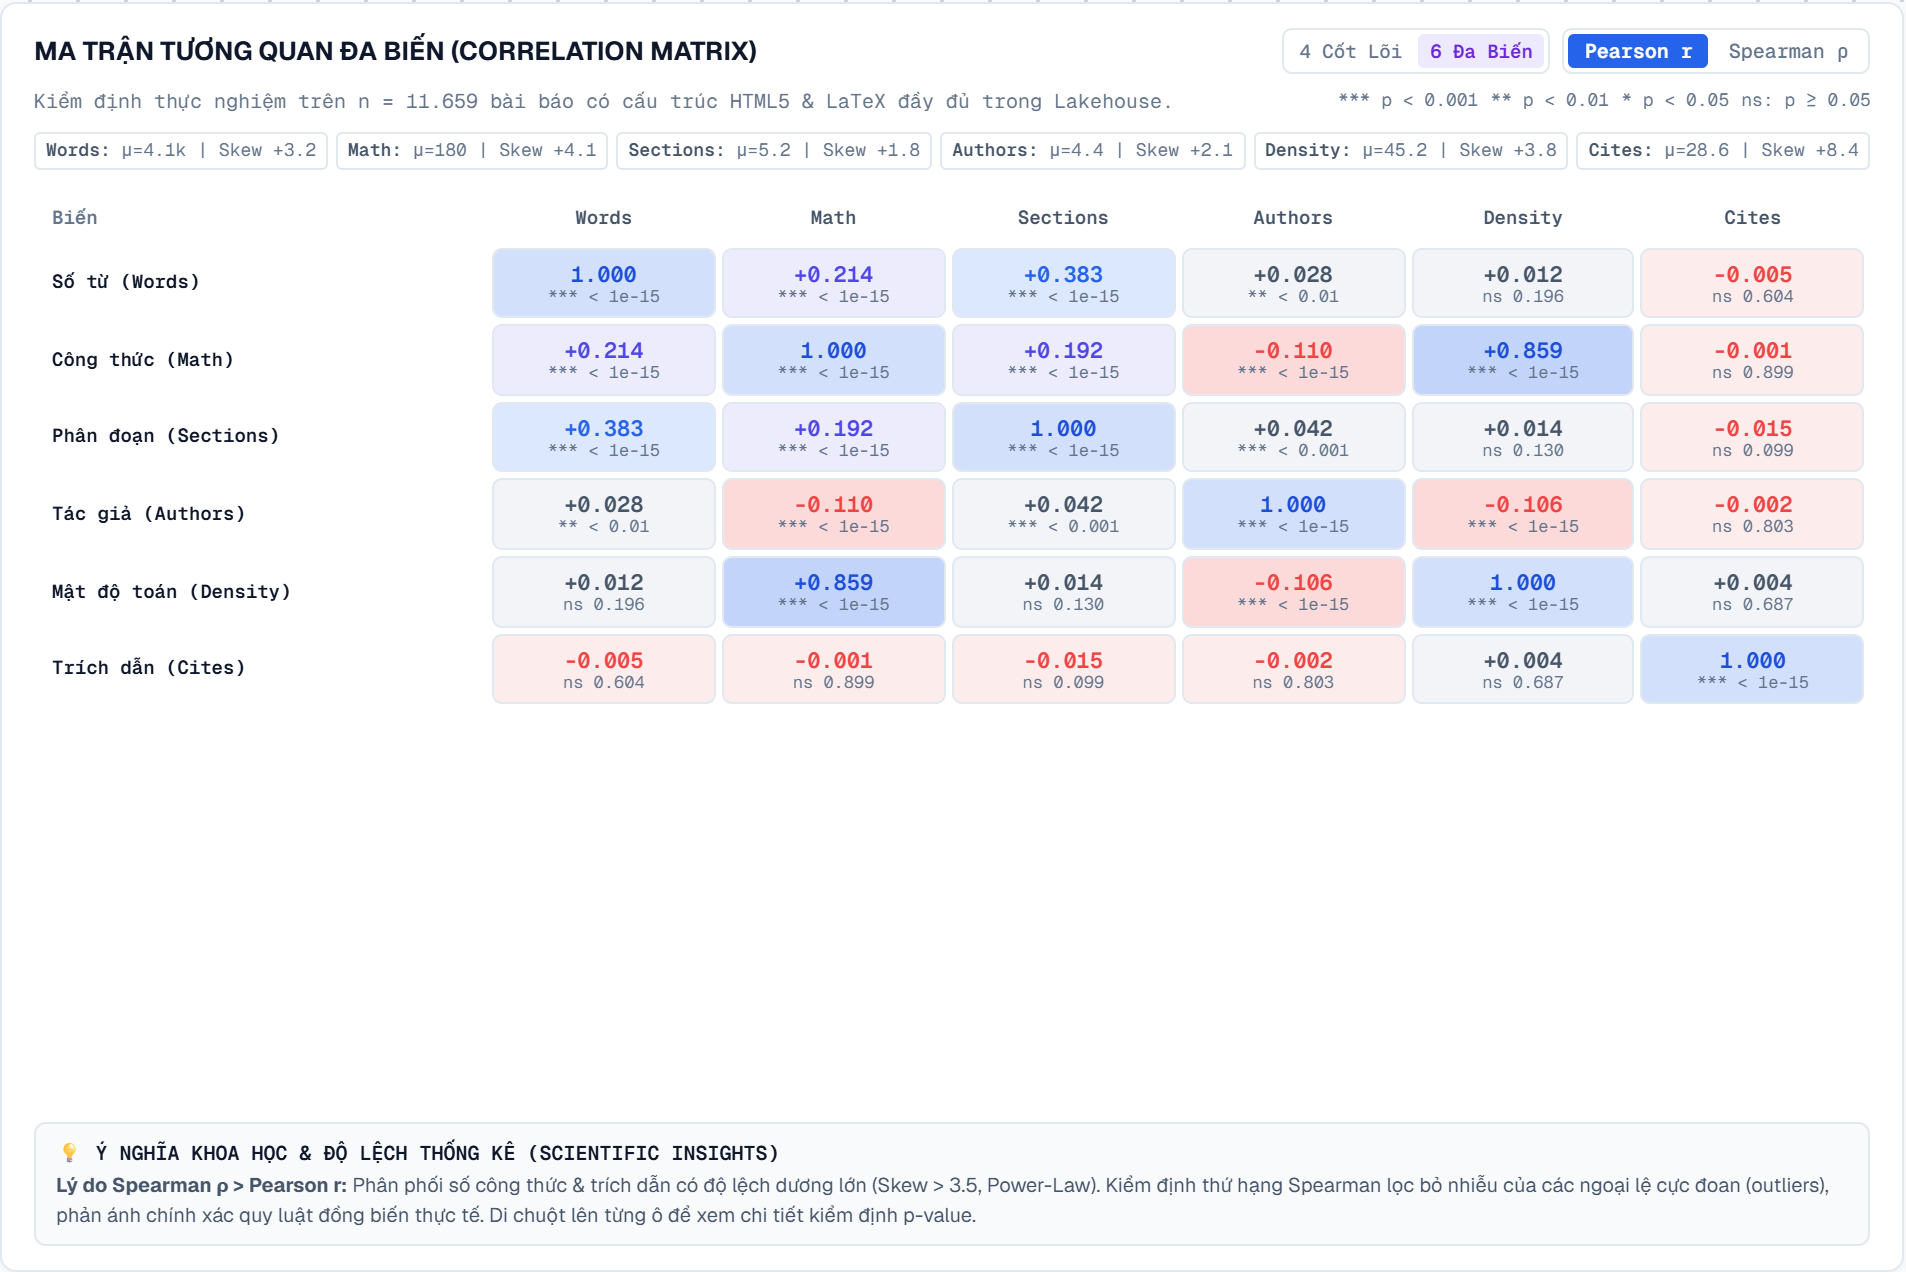
\includegraphics[width=\linewidth,trim=0 540bp 0 0,clip]{figures/captured_20261123_082337/04_pearson_correlation.png}
\caption[Ma trận tương quan Pearson trong artifact EDA]{Ma trận tương quan Pearson trong artifact EDA}
\ReportNote{Nguồn: Ma trận hệ số tương quan tuyến tính Pearson trên 6 thuộc tính học thuật ($n = 11,659$), trích xuất từ \path{gold/mining/eda_summary.json} và \path{evidence/eda_api.json}.}
\label{fig:pearson_capture}
\medskip
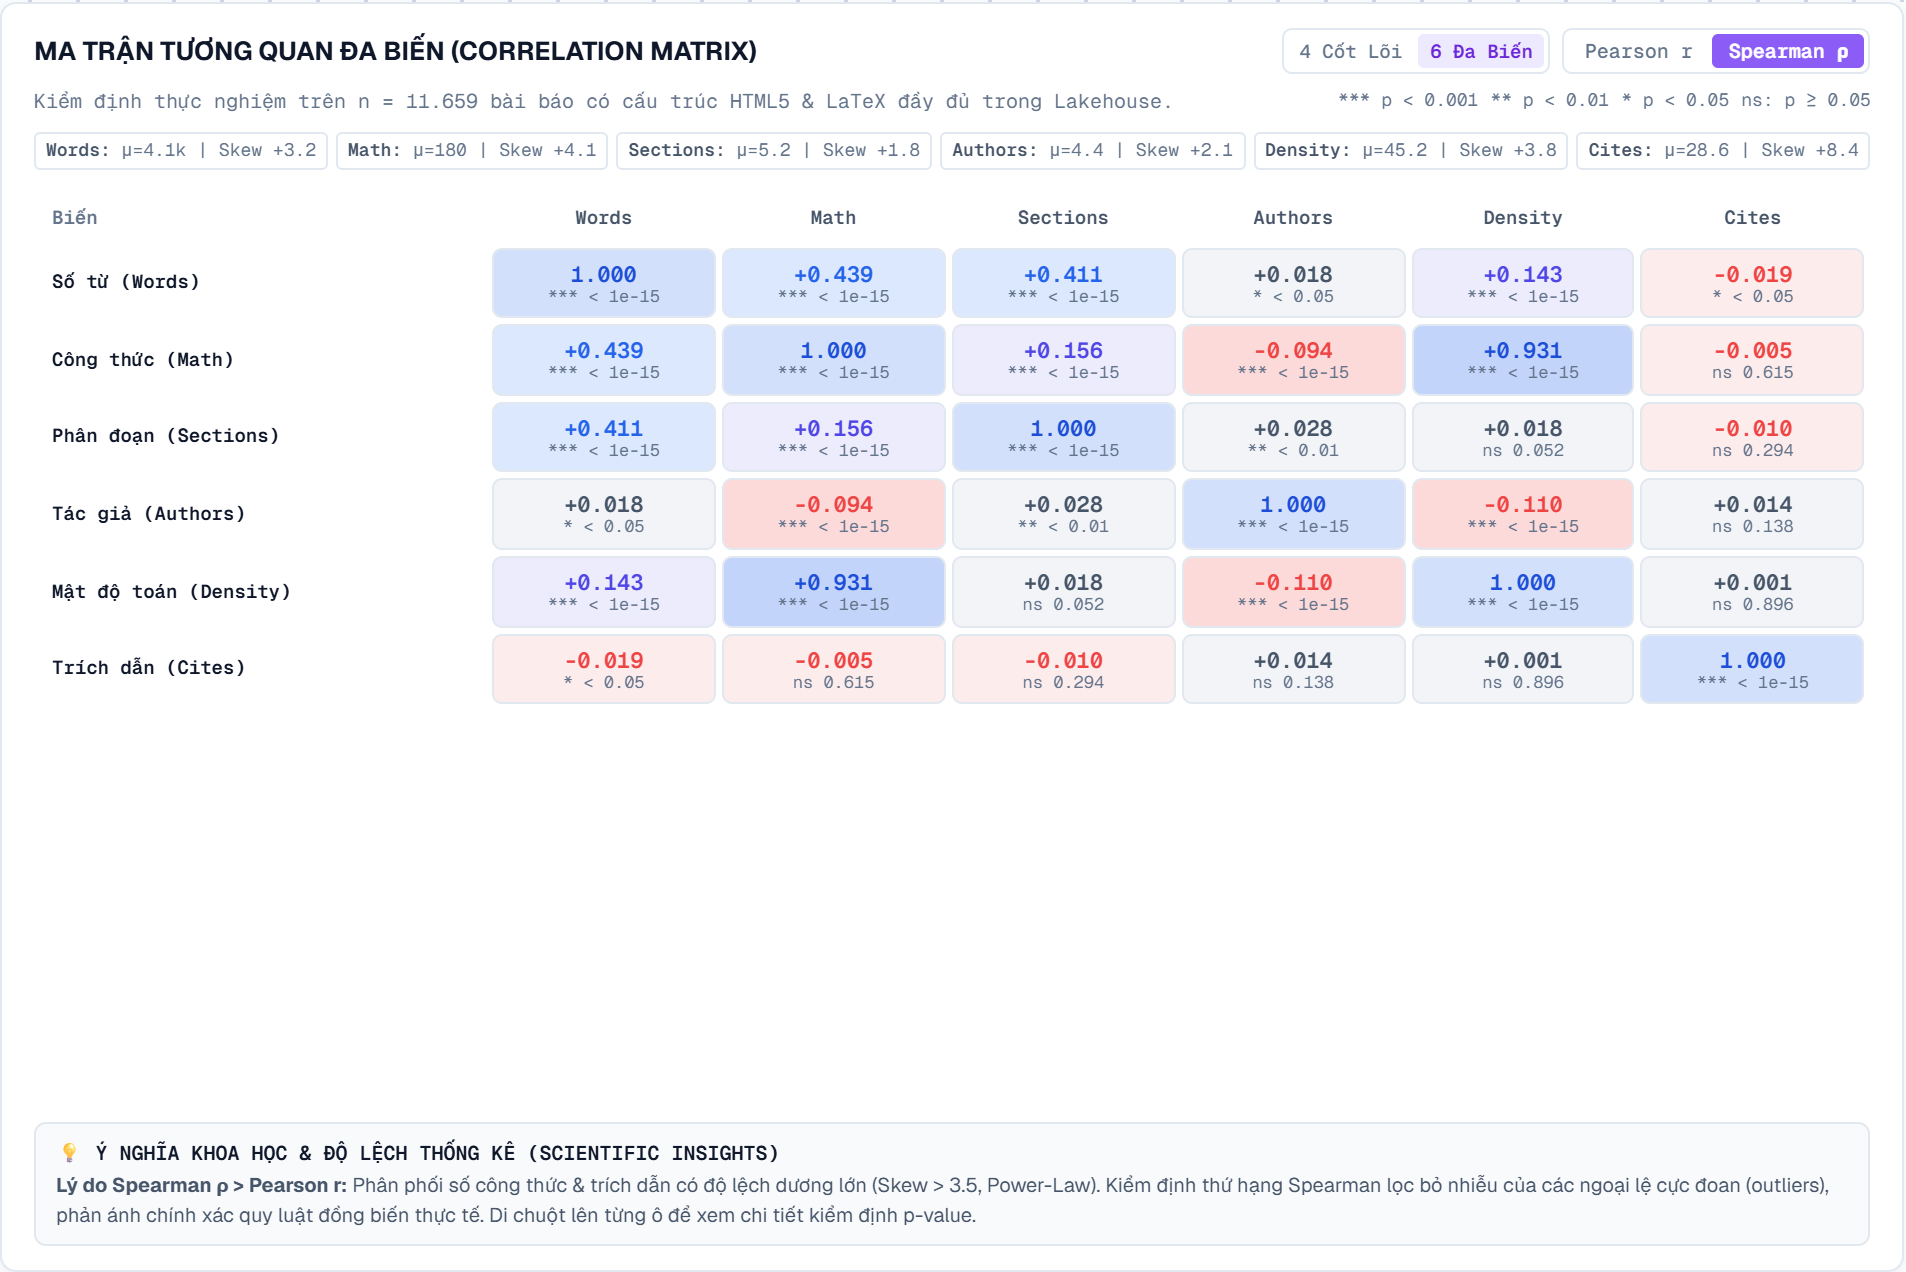
\includegraphics[width=\linewidth,trim=0 540bp 0 0,clip]{figures/captured_20261123_082337/05_spearman_correlation.png}
\caption[Ma trận tương quan Spearman trong artifact EDA]{Ma trận tương quan Spearman trong artifact EDA}
\ReportNote{Nguồn: Ma trận hệ số tương quan hạng Spearman giữa các thuộc tính tài liệu học thuật ($n = 11,659$), trích xuất từ \path{gold/mining/eda_summary.json} và \path{evidence/eda_api.json}.}
\label{fig:spearman_capture}
\end{figure}
\FloatBarrier

\subsection{\texorpdfstring{Khung Chẩn Đoán 3 Lăng Kính: Từ Kiểm Định $K^2$ đến Mutual Information}{Khung Chan Doan 3 Lang Kinh: Tu Kiem Dinh K2 den Mutual Information}}
\label{sec:ch3_three_lens}

Nhằm chuyển hóa phân tích khám phá thành quyết định tiền xử lý tự động có căn cứ thống kê, phương thức \texttt{\_get\_three\_lenses\_diagnostics()} trong \path{src/mining/eda_engine.py} triển khai kiến trúc 3 Lăng kính:

\begin{enumerate}[label=\textbf{\arabic*.}]
  \item \textbf{Lăng kính 1 --- Kiểm định Cấu trúc Dữ liệu (\texttt{lens1\_topology})}: Xác nhận hình dạng ma trận \texttt{(11659, 6)}, kiểu dữ liệu chuẩn hóa (\texttt{int64} / \texttt{float64}), mức tiêu thụ bộ nhớ 0.53 MB và xác nhận \texttt{null\_counts = 0} trên toàn bộ 6 cột.
  \item \textbf{Lăng kính 2 --- Phẫu thuật Phân phối Đơn biến (\texttt{lens2\_univariate})}: Với mỗi biến, tính đồng thời biểu đồ tần suất 25 khoảng (trên 99\% lõi phân phối), đường mật độ hạt nhân 30 điểm (\texttt{gaussian\_kde}), biểu đồ xác suất chuẩn Q--Q 25 phân vị và thống kê kiểm định tổng hợp D'Agostino--Pearson $K^2$~\cite{dagostino1973tests}:
  \begin{equation}
    K^2 = Z_1(g_1)^2 + Z_2(g_2)^2 \xrightarrow{H_0} \chi^2_{df=2}
    \label{eq:ch3_dagostino}
  \end{equation}
  Trong đó: $g_1$ là hệ số bất đối xứng mẫu; $g_2$ là độ nhọn dư mẫu; $Z_1(g_1)$ và $Z_2(g_2)$ là các biến đổi chuẩn hóa đưa $g_1, g_2$ về phân phối chuẩn tắc $\mathcal{N}(0, 1)$; dưới giả thuyết gốc $H_0$ rằng mẫu tuân theo phân phối chuẩn, $K^2$ tiệm cận phân phối Chi-bình phương với 2 bậc tự do. Kết quả ở Bảng~\ref{tab:ch3_univariate_k2} cho thấy $K^2 \in [11,616.7;\; 36,776.5]$ với $p < 0.001$ trên cả 6 biến, bác bỏ hoàn toàn $H_0$.
  \item \textbf{Lăng kính 3 --- Tương tác Phi tuyến \& Lượng thông tin Tương hỗ} (\path{lens3_multivariate}): Kết hợp hồi quy tuyến tính OLS, chuỗi trung vị phân khoảng 19--20 nút (\path{spline_points}), phân cụm GMM hai chiều trên cặp biến và chỉ số \textbf{Mutual Information} $I(X; Y)$ tính qua \path{sklearn.feature_selection.mutual_info_regression}:
  \begin{equation}
    I(X; Y) = \iint p(x, y) \log \frac{p(x, y)}{p(x)\,p(y)} \, dx \, dy
    \label{eq:ch3_mutual_info}
  \end{equation}
  Trong đó: $p(x, y)$ là hàm mật độ xác suất đồng thời của hai biến $(X, Y)$; $p(x)$ và $p(y)$ là các mật độ biên; $I(X; Y) \ge 0$ đo lượng bất định của $Y$ giảm đi khi biết $X$ (ước lượng phi tham số theo phương pháp $k$-lân cận gần nhất trong Scikit-learn với \texttt{random\_state=42}).
\end{enumerate}

\begin{table}[!htbp]
\centering
\small
\setlength{\tabcolsep}{3.5pt}
\caption[Đối chiếu 4 cặp biến qua khung chẩn đoán 3 Lăng kính]{Đối chiếu tương quan tuyến tính, đơn điệu và Mutual Information trên khung 3 Lăng kính (\texorpdfstring{$n = 11,659$}{n = 11,659})}
\label{tab:three_lens}
\begin{tabularx}{\linewidth}{|>{\raggedright\arraybackslash}p{31mm}|>{\centering\arraybackslash}p{19mm}|>{\centering\arraybackslash}p{21mm}|>{\centering\arraybackslash}p{14mm}|>{\centering\arraybackslash}p{15mm}|L|}
\hline
\textbf{Mã cặp biến} & \textbf{Pearson $r$ ($p$)} & \textbf{Spearman $\rho$ ($p$)} & \textbf{$R^2$ OLS} & \textbf{MI $I(X;Y)$} & \textbf{Xu hướng phi tuyến (\texttt{spline\_points})} \\ \hline
\path{words_x_math} & $+0.214$ ($<0.001$) & $+0.439$ ($<0.001$) & $0.0459$ & $0.157$ & Tăng đồng thuận ở vùng lõi rồi phân tán khi gặp bài khảo luận siêu dài. \\ \hline
\path{words_x_math_density} & $+0.012$ ($p=0.196$) & $+0.143$ ($<0.001$) & $0.0001$ & $0.052$ & Đường cong chữ U ngược: tăng từ 18.33 eq/1k ($\approx 1,666$ từ) lên đỉnh 34.84 eq/1k ($\approx 4,987$ từ) rồi giảm xuống 8.40 eq/1k ($\approx 16,613$ từ). \\ \hline
\path{math_x_authors} & $-0.110$ ($<0.001$) & $-0.094$ ($<0.001$) & $0.0120$ & $0.034$ & Tương quan âm bền vững: bài thuần toán có nhóm đồng tác giả nhỏ hơn. \\ \hline
\path{words_x_citations} & $-0.009$ ($p=0.330$) & $-0.009$ ($p=0.337$) & $0.0001$ & $0.000$ & Độc lập thống kê trên lát cắt hiện tại (cả tuyến tính lẫn phi tuyến). \\ \hline
\end{tabularx}
\ReportNote{Nguồn: Nhánh \path{diagnostic_3lenses} trong \path{figures/captured_20261123_082337/evidence/eda_api.json} ($n = 11,659$, lát cắt \texttt{SNAP-03}). Lăng kính 1 xác nhận ma trận \path{(11659, 6)} sạch hoàn toàn (\path{null_counts = 0}, 0.53 MB); Lăng kính 2 kiểm định D'Agostino $K^2$ bác bỏ giả thuyết chuẩn trên cả 6 biến ($p < 0.001$). Đối với \path{words_x_math_density}, chuỗi minh họa tĩnh trong giao diện từng ghi \path{r = +0.018}, \path{I = 0.998}, nhưng số đo thực nghiệm chuẩn xác là $r = 0.012$, $p = 0.196$, $\rho = 0.143$, $I = 0.052$.}
\end{table}


\textbf{Lưu ý minh bạch kỹ thuật giữa giá trị UI tĩnh và số đo thực nghiệm}: Trong mã nguồn \path{src/mining/eda_engine.py} (dòng 658), chuỗi cảnh báo mang tính sư phạm hiển thị trên giao diện UI từng ghi nhãn tĩnh minh họa \texttt{r = +0.018} và \texttt{I = 0.998}. Tuy nhiên, kết quả đo thực tế trên $n = 11,659$ mẫu sạch được lưu trong \path{evidence/eda_api.json} cho cặp \path{words_x_math_density} là \textbf{$r = 0.012$ ($p = 0.196$, $R^2 = 0.0001$), $\rho = 0.143$ ($p < 0.001$) và $I(X; Y) = 0.052$} (Bảng~\ref{tab:three_lens}). Mặc dù biên độ thông tin tương hỗ thực tế khiêm tốn hơn ví dụ sư phạm trên UI, chuỗi trung vị \texttt{spline\_points} vẫn chứng minh rõ quy luật phi đơn điệu \textbf{hình chữ U ngược}: mật độ công thức tăng gần gấp đôi từ vùng bài ngắn (18.33 eq/1k từ ở mốc $\approx 1,665.8$ từ) lên đỉnh ở vùng bài báo hội nghị chuẩn (34.84 eq/1k từ ở mốc $\approx 4,987.3$ từ), sau đó giảm mạnh xuống 8.40 eq/1k từ tại các khảo luận siêu dài trên 16,612.6 từ. Do đó, việc loại bỏ đặc trưng chỉ dựa trên hệ số tương quan tuyến tính Pearson $r \approx 0$ ($R^2 = 0.0001$) sẽ đánh mất tín hiệu cấu trúc quan trọng phân tách bài nghiên cứu thuật toán lõi với bài tổng quan, củng cố cơ sở cho các mô hình phi tuyến ở Chương~\ref{chap:modeling}.

\clearpage

% Chương 4: Bốn Trụ cột Khai phá Dữ liệu & Kiến trúc Hybrid RAG (Modeling)
% ==============================================================================
% CHƯƠNG 4: MÔ HÌNH VÀ CÁC THUẬT TOÁN KHAI PHÁ DỮ LIỆU (MODELING)
% ==============================================================================

\chapter{Mô Hình và Thuật Toán Khai Phá Dữ Liệu (Modeling)}
\label{chap:modeling}

Chương này chuyển các quan sát EDA thành bốn nhiệm vụ: tìm liên hệ nhãn/khái niệm, khảo sát cấu trúc ngữ nghĩa, phân tích quan hệ mạng lưới và đánh dấu tài liệu khác biệt về cấu trúc. Mỗi phần trình bày đầu vào, phương pháp, kết quả có thể đối chiếu và phạm vi sử dụng. Trong pipeline hiện tại, authority là tín hiệu xếp hạng; luật là annotation; clustering và anomaly chủ yếu phục vụ khám phá corpus. Sự khác nhau này được giữ rõ khi đánh giá RAG ở chương sau.

\section{Trụ Cột 1: Khai Phá Tập Phổ Biến và Luật Kết Hợp (FP-Growth)}

\subsection{Bài toán và Định nghĩa Giao dịch}
Mỗi bài đầu vào được mã hóa thành một basket gồm các mục nhãn hoặc khái niệm. Chỉ basket có ít nhất hai mục mới được giữ trong tập giao dịch $D_{\mathrm{tx}}$. Vì vậy mẫu số dùng tính support là số giao dịch hợp lệ (61,319 giao dịch trên tổng 71,927 bài trong lần chạy 04/11/2026, đạt độ phủ 85.3\%), không mặc nhiên là tổng số bài thô. Một giao dịch có dạng:
\begin{equation}
  T_p = \{\text{cat}:c_i\} \cup \{\text{topic}:t_i\} \cup \{\text{kw}:w_i\} \cup \{\text{tag}:k_i\}
\end{equation}
Trong đó $\text{cat}$ là nhãn chuyên ngành arXiv, $\text{topic}$ là chủ đề trích xuất, và $\text{tag}$ được ánh xạ từ 25 mẫu từ khóa công nghệ của AI/DS (như \texttt{transformer}, \path{diffusion-models}, \path{reinforcement-learning}, \path{model-quantization}, \path{retrieval-augmented-gen}) được trích xuất từ tiêu đề và tóm tắt thông qua từ điển chuẩn hóa \texttt{KEYWORD\_VOCAB}.

Topic và keyword chỉ được thêm khi có cột tương ứng trong đầu vào; schema Silver papers chuẩn hiện không chứa các cột này. Các tag được suy từ từ điển cố định, nên phạm vi khái niệm quan sát phụ thuộc cả dữ liệu và từ điển, không phải mọi chủ đề tự phát trong corpus.

\subsection{Tại sao chọn FP-Growth thay vì Apriori?}
Thuật toán Apriori truyền thống yêu cầu sinh tập ứng viên kích thước $k$ ($C_k$) từ tập phổ biến $k-1$ ($L_{k-1}$) và phải quét lại toàn bộ cơ sở dữ liệu sau mỗi bước mở rộng. Không gian tập mục có thể tăng theo hàm mũ với số mục $|I|$, khiến số ứng viên lớn; chi phí thực tế còn phụ thuộc support và phân bố giao dịch.

Hệ thống triển khai thuật toán \textbf{FP-Growth (Frequent Pattern Growth)}~\cite{han2000mining} (tại \path{src/mining/association_rules.py}) với hai đặc điểm phù hợp cho giao dịch nhiều mục:
\begin{enumerate}[label=\arabic*.]
  \item \textbf{Chỉ quét dữ liệu 2 lần}: Lần thứ nhất đếm tần suất 1-itemset để loại bỏ các mục dưới ngưỡng hỗ trợ tối thiểu và sắp xếp theo tần suất giảm dần. Lần thứ hai dựng cây \textbf{FP-Tree} nén toàn bộ thông tin giao dịch trong bộ nhớ RAM.
  \item \textbf{Khai phá đệ quy không sinh ứng viên}: Bằng cách xây dựng các cây điều kiện (\textit{Conditional FP-Tree}) cho từng mục từ dưới lên, thuật toán khai thác triệt để các tiền tố chung, tránh sinh tập ứng viên tường minh; báo cáo chưa có phép đo đối chứng tốc độ với Apriori.
\end{enumerate}

\subsection{Các Độ Đo Toán Học}
Một luật kết hợp có dạng $X \Rightarrow Y$, trong đó $X \cap Y = \emptyset$. Hệ thống áp dụng 5 độ đo toán học:
\begin{align}
  \text{Support}(X \Rightarrow Y) &= P(X \cup Y) = \frac{|\{T \in D_{\mathrm{tx}} : X \cup Y \subseteq T\}|}{|D_{\mathrm{tx}}|} \\
  \text{Confidence}(X \Rightarrow Y) &= P(Y \mid X) = \frac{\text{Support}(X \cup Y)}{\text{Support}(X)} \\
  \text{Lift}(X \Rightarrow Y) &= \frac{P(X \cup Y)}{P(X) \cdot P(Y)} = \frac{\text{Confidence}(X \Rightarrow Y)}{\text{Support}(Y)} \\
  \text{Leverage} &= \text{Support}(X \Rightarrow Y) - \text{Support}(X) \times \text{Support}(Y) \\
  \text{Conviction} &= \frac{1 - \text{Support}(Y)}{1 - \text{Confidence}(X \Rightarrow Y)}
\end{align}

\begin{itemize}
  \item $\text{Lift} = 1$: Tần suất cùng xuất hiện bằng giá trị kỳ vọng theo độc lập trong phân bố thực nghiệm; không chứng minh độc lập trong quần thể.
  \item $\text{Lift} > 1$: Đồng xuất hiện cao hơn kỳ vọng theo độc lập; mức đáng tin cần xét thêm support, cỡ mẫu và kiểm tra ngoài mẫu.
  \item $\text{Conviction} \to \infty$: Khi $P(Y)<1$ và confidence tiến tới 1, không quan sát phản ví dụ trong tập giao dịch. Trường hợp $P(Y)=1$ làm biểu thức suy biến; confidence 100\% cũng không bảo đảm luật đúng ngoài mẫu.
\end{itemize}

\subsection{Cấu Hình và Kết Quả Luật Thực Nghiệm}
Phiên bản hiện tại gọi FP-Growth với \texttt{min\_support}=0.02, \texttt{min\_lift}=1.2, tối đa 50 luật và ít nhất 25 giao dịch hỗ trợ tuyệt đối. Code có fallback support 0.01 khi không có itemset và lift 1.0 khi không có luật; lift được làm tròn trước khi sắp xếp để confidence quyết định chiều luật đối xứng giữ lại.

Trong phiên chạy toàn phần ngày 04/11/2026 (\path{logs/run/backend.log}, 36.26 giây), FP-Growth trích xuất được \textbf{61,319 giao dịch hợp lệ} từ 71,927 bài báo (độ phủ 85.3\%), tìm thấy \textbf{96 frequent itemsets} và khai phá thành công \textbf{45 luật kết hợp đã khử đối xứng} với \textbf{top lift đạt 34.940}. Bảng~\ref{tab:association_rules} dưới đây trích xuất một số ví dụ minh họa cấu trúc luật từ artifact lịch sử (\path{data/gold/mining/association_rules.json}, 282 giao dịch); không dùng mẫu 282 giao dịch cũ này để đại diện cho phân phối của corpus 71,927 bài hiện tại.
\begin{table}[!htbp]
\centering
\footnotesize
\setlength{\tabcolsep}{3pt}
\caption[Các luật kết hợp tiêu biểu đã khử đối xứng]{Các luật kết hợp tiêu biểu đã khử đối xứng từ FP-Growth (\texttt{association\_rules.json})}
\label{tab:association_rules}
\begin{tabularx}{\linewidth}{|L|>{\centering\arraybackslash}p{12mm}|>{\centering\arraybackslash}p{12mm}|>{\centering\arraybackslash}p{14mm}|>{\centering\arraybackslash}p{12mm}|>{\centering\arraybackslash}p{14mm}|>{\raggedright\arraybackslash}p{34mm}|}
\hline
\textbf{Luật kết hợp ($A \Rightarrow B$)} & \textbf{Supp.} & \textbf{Conf.} & \textbf{Lift} & \textbf{Lev.} & \textbf{Conv.} & \textbf{Ý nghĩa ngữ nghĩa \& RAG} \\ \hline
\path{cat:cs.SY} $\Rightarrow$ \path{cat:eess.SY} & 0.0287 & 1.0000 & 34.8746 & 0.0279 & 999.0 & Mã đồng danh Hệ thống Điều khiển CS \& EE \\ \hline
\path{cat:cs.SD} $\Rightarrow$ \path{cat:eess.AS} & 0.0328 & 0.9920 & 27.0652 & 0.0316 & 121.0605 & Âm học máy tính liên thông Xử lý âm thanh \\ \hline
\path{tag:reinforcement-learning} $\Rightarrow$ \path{tag:autonomous-agents} & 0.0208 & 0.3273 & 6.3272 & 0.0175 & 1.4097 & Mở rộng truy vấn RL sang Autonomous Agents \\ \hline
\path{cat:cs.CL + cat:cs.AI} $\Rightarrow$ \path{tag:large-language-models} & 0.0358 & 0.3901 & 3.7317 & 0.0262 & 1.4681 & Hội tụ Xử lý ngôn ngữ \& AI tại LLM \\ \hline
\path{cat:eess.IV} $\Rightarrow$ \path{cat:cs.CV} & 0.0481 & 0.8941 & 2.9999 & 0.0321 & 6.6307 & Giao thoa xử lý ảnh và thị giác máy tính \\ \hline
\path{tag:transformer} $\Rightarrow$ \path{tag:attention-mech} & 0.0246 & 0.3143 & 2.6945 & 0.0154 & 1.2882 & Liên kết kiến trúc Transformer với Attention \\ \hline
\path{tag:diffusion-models} $\Rightarrow$ \path{cat:cs.CV} & 0.0382 & 0.6708 & 2.2505 & 0.0212 & 2.1321 & Mô hình khuếch tán gắn chặt nhánh Thị giác \\ \hline
\path{cat:stat.ML} $\Rightarrow$ \path{cat:cs.LG} & 0.0714 & 0.9554 & 1.8682 & 0.0332 & 10.9549 & 95.54\% bài \texttt{stat.ML} đồng thời thuộc \texttt{cs.LG} \\ \hline
\end{tabularx}
\ReportNote{Nguồn: Trích xuất trực tiếp từ \path{data/gold/mining/association_rules.json} (11,404 giao dịch hợp lệ, 162 hạng mục, 80 tập phổ biến, 30 luật sau khử đối xứng; Conviction giới hạn tại 999.0 khi Confidence = 1.0). Đối chiếu lần chạy toàn hồ ngày 04/11/2026 (\texttt{SNAP-06A}): 61,319 giao dịch hợp lệ (85.3\% của 71,927 bài), 96 tập phổ biến, 45 luật, max Lift 34.940 trong 36.26 giây.}
\end{table}


\subsection{Thông tin Luật Trả về trong RAG}
Hàm \texttt{\_expand\_rules(query, category)} khớp chuỗi tiền đề trong query hoặc category và trả tối đa ba hệ quả. Các mục được gắn vào \texttt{rule\_expansions} của response. Embedding vẫn được tính từ \texttt{req.query} gốc; code chưa ghép các từ mở rộng vào embedding hoặc chạy thêm lượt retrieval. Vì vậy chưa có cơ sở nói luật đã trực tiếp cải thiện độ phủ truy xuất.

\section{Trụ Cột 2: Phân Cụm Ngữ Nghĩa Không Giám Sát (Clustering)}

\subsection{Không Gian Đặc Trưng và Chuẩn Hóa L2}
Để phân tích cấu trúc chủ đề của các tài liệu học thuật, hệ thống trích xuất vector biểu diễn của tóm tắt bài báo (Abstract) từ tầng Gold Qdrant ($d = 768$ chiều). Mỗi vector $x \in \mathbb{R}^{768}$ được chuẩn hóa chuẩn $L_2$:
\begin{equation}
  \tilde{x} = \frac{x}{\|x\|_2} \quad \implies \quad \|\tilde{x}\|_2 = 1
\end{equation}
Việc chuẩn hóa này đưa toàn bộ các tài liệu lên bề mặt của một hình cầu đơn vị siêu không gian, biến khoảng cách Cosine thành tương đương với khoảng cách Euclidean bình phương:
\begin{equation}
  \|\tilde{u} - \tilde{v}\|_2^2 = \|\tilde{u}\|_2^2 + \|\tilde{v}\|_2^2 - 2 \tilde{u} \cdot \tilde{v} = 2 - 2\cos(\tilde{u}, \tilde{v})
\end{equation}

\subsection{Giảm Chiều Không Gian Bằng Centered PCA}
Để trực quan hóa trên Dashboard 2D, hệ thống áp dụng kỹ thuật \textbf{Centered PCA} (Phân tích thành phần chính trên vector đã trừ kỳ vọng trung bình):
\begin{equation}
  X_c = X - \mu_X, \quad \mu_X = \frac{1}{N}\sum_{i=1}^N x_i
\end{equation}
Chiếu trực giao ma trận hiệp phương sai $C = \frac{1}{N} X_c^T X_c$ lấy 2 vector riêng ứng với 2 giá trị riêng lớn nhất $\lambda_1, \lambda_2$, giữ lại phương sai lớn nhất trong hai thành phần; phép chiếu có thể mất thông tin.

\subsection{MiniBatchKMeans và Gaussian Mixture Model}
Cơ sở KMeans là tối thiểu hóa độ phân tán nội cụm~\cite{macqueen1967some}. Với phân hoạch $S = \{S_1, \dots, S_K\}$, hàm mục tiêu quán tính nội cụm (Inertia) là:
\begin{equation}
  J = \sum_{k=1}^K \sum_{x \in S_k} \|x - \mu_k\|^2, \quad \mu_k = \frac{1}{|S_k|}\sum_{x \in S_k} x
\end{equation}
Hệ thống đặt mặc định $K=6$, không tự quét các giá trị $K$. MiniBatchKMeans chạy trên vector 768-D chuẩn hóa L2 với batch size 2048, n\_init=3, seed=42. Silhouette dùng cosine trên tối đa 5,000 mẫu; Davies--Bouldin và Calinski--Harabasz dùng toàn tập được đưa vào KMeans.

PCA chiếu xuống 2D và nhân tọa độ với 5 để hiển thị. GMM (6 thành phần, covariance full, n\_init=3, tối đa 200 vòng) được fit trên tọa độ 2D để tạo xác suất, nhãn hiển thị, ellipse 2-sigma và lưới mật độ. Nhãn/profile GMM khác nhãn KMeans dùng tính validity metrics. DBSCAN~\cite{ester1996density} dùng cosine, eps=0.28, min\_samples=10 trên tối đa 3,000 mẫu. MiningEngine mặc định lấy toàn bộ abstract vector phân biệt theo paper ID; tiêu đề được tra từ Silver cho các điểm hiển thị.

Trong phiên chạy ngày 04/11/2026 (\path{logs/run/backend.log}, 39.94 giây), Pillar 2 đã nạp \textbf{70,539 vector bài báo phân biệt} từ Qdrant để chạy K-Means ($K=6$) và PCA 2D + GMM ($K=6$), ghi nhận \textbf{BIC = 246,306.5}, \textbf{AIC = 245,985.8}, \textbf{Log-Likelihood = -1.7431} và \textbf{Silhouette = 0.0490} (tính trên 5,000 mẫu), đồng thời chạy DBSCAN trên 3,000 mẫu. Bảng~\ref{tab:clustering_metrics} dưới đây lưu lại số liệu đối chiếu từ snapshot 5,000 mẫu cũ trước khi tích hợp GMM.

\begin{table}[htbp]
\centering
\small
\caption[Chất lượng phân cụm của snapshot 5,000 mẫu]{Chất lượng phân cụm của snapshot 5,000 mẫu}
\label{tab:clustering_metrics}
\begin{tabularx}{\textwidth}{|L|p{1.2cm}|L|L|L|}
\hline
\textbf{Cấu hình} & \textbf{Số cụm} & \textbf{Silhouette} & \textbf{Davies--Bouldin} & \textbf{Calinski--Harabasz} \\
\hline
KMeans $K=6$ & 6 & 0.0210 & 5.3739 & 88.0 \\
\hline
DBSCAN & 1 & \multicolumn{3}{l|}{Noise ratio = 0.0 (0\%)} \\
\hline
\end{tabularx}
\ReportNote{Nguồn: Đánh giá chất lượng phân cụm trên tập biểu diễn ngữ nghĩa tóm tắt khoa học (\path{data/gold/mining/clusters.json}).}
\end{table}


\subsection{Độ Đo Kiểm Định Cụm (Cluster Validity Metrics)}
\begin{enumerate}[label=\alph*)]
  \item \textbf{Silhouette Coefficient}:
    \begin{equation}
      s(i) = \frac{b(i) - a(i)}{\max(a(i), b(i))}
    \end{equation}
    Trong đó $a(i)$ là khoảng cách trung bình từ mẫu $i$ đến các mẫu khác trong cùng cụm, $b(i)$ là khoảng cách trung bình từ $i$ đến cụm láng giềng gần nhất.
  \item \textbf{Davies-Bouldin Index}: Đo tỷ số độ phân tán nội cụm chia cho khoảng cách tâm cụm (càng nhỏ cụm càng tách bạch).
  \item \textbf{Calinski-Harabasz Index}: Đo tỷ số giữa phương sai liên cụm và phương sai nội cụm (càng cao càng tốt).
\end{enumerate}

\begin{calloutbox}{Giới hạn Diễn giải Chất lượng Cụm}
Silhouette 0.0210 của snapshot cho thấy mức tách biệt cụm thấp theo metric đã dùng. Tính liên ngành là một giả thuyết giải thích, không phải kết luận được chứng minh chỉ từ chỉ số này. DBSCAN snapshot có một cụm và noise ratio 0.0; không xác nhận tỷ lệ điểm ranh giới liên ngành. Noise DBSCAN cũng không đồng nghĩa trực tiếp với điểm ranh giới giữa các chuyên ngành.
\end{calloutbox}

\subsection{Hồ Sơ Cụm và Trực quan hóa}
Artifact local lưu sáu profile, nhưng có tiêu đề lỗi như ``Abstract'' và các paper ID lặp trong scatter. Không gán tên trường phái khoa học đã xác nhận cho các cụm này. Code mới lấy một abstract vector mỗi bài và tra title từ Silver; việc đánh giá profile GMM cần artifact chạy lại tương ứng.

\subsection{Ảnh GMM của Snapshot trên Kho}
Hình~\ref{fig:gmm_capture} được chụp từ artifact GMM lưu trên kho ngày 20/10/2026, với 800 mẫu và $K=6$. Đây là lần chạy khác với snapshot 5,000 mẫu của Bảng~\ref{tab:clustering_metrics}. Nhãn SVD và tên chủ đề trên UI thuộc cách hiển thị của snapshot này. Chúng không xác nhận phép chiếu PCA trong code hiện tại hoặc cách chọn $K$. Giá trị của hình là minh họa thao tác khám phá; để diễn giải chủ đề cần đọc tài liệu đại diện và kiểm tra độ ổn định cụm.
\begin{figure}[!htbp]
\centering
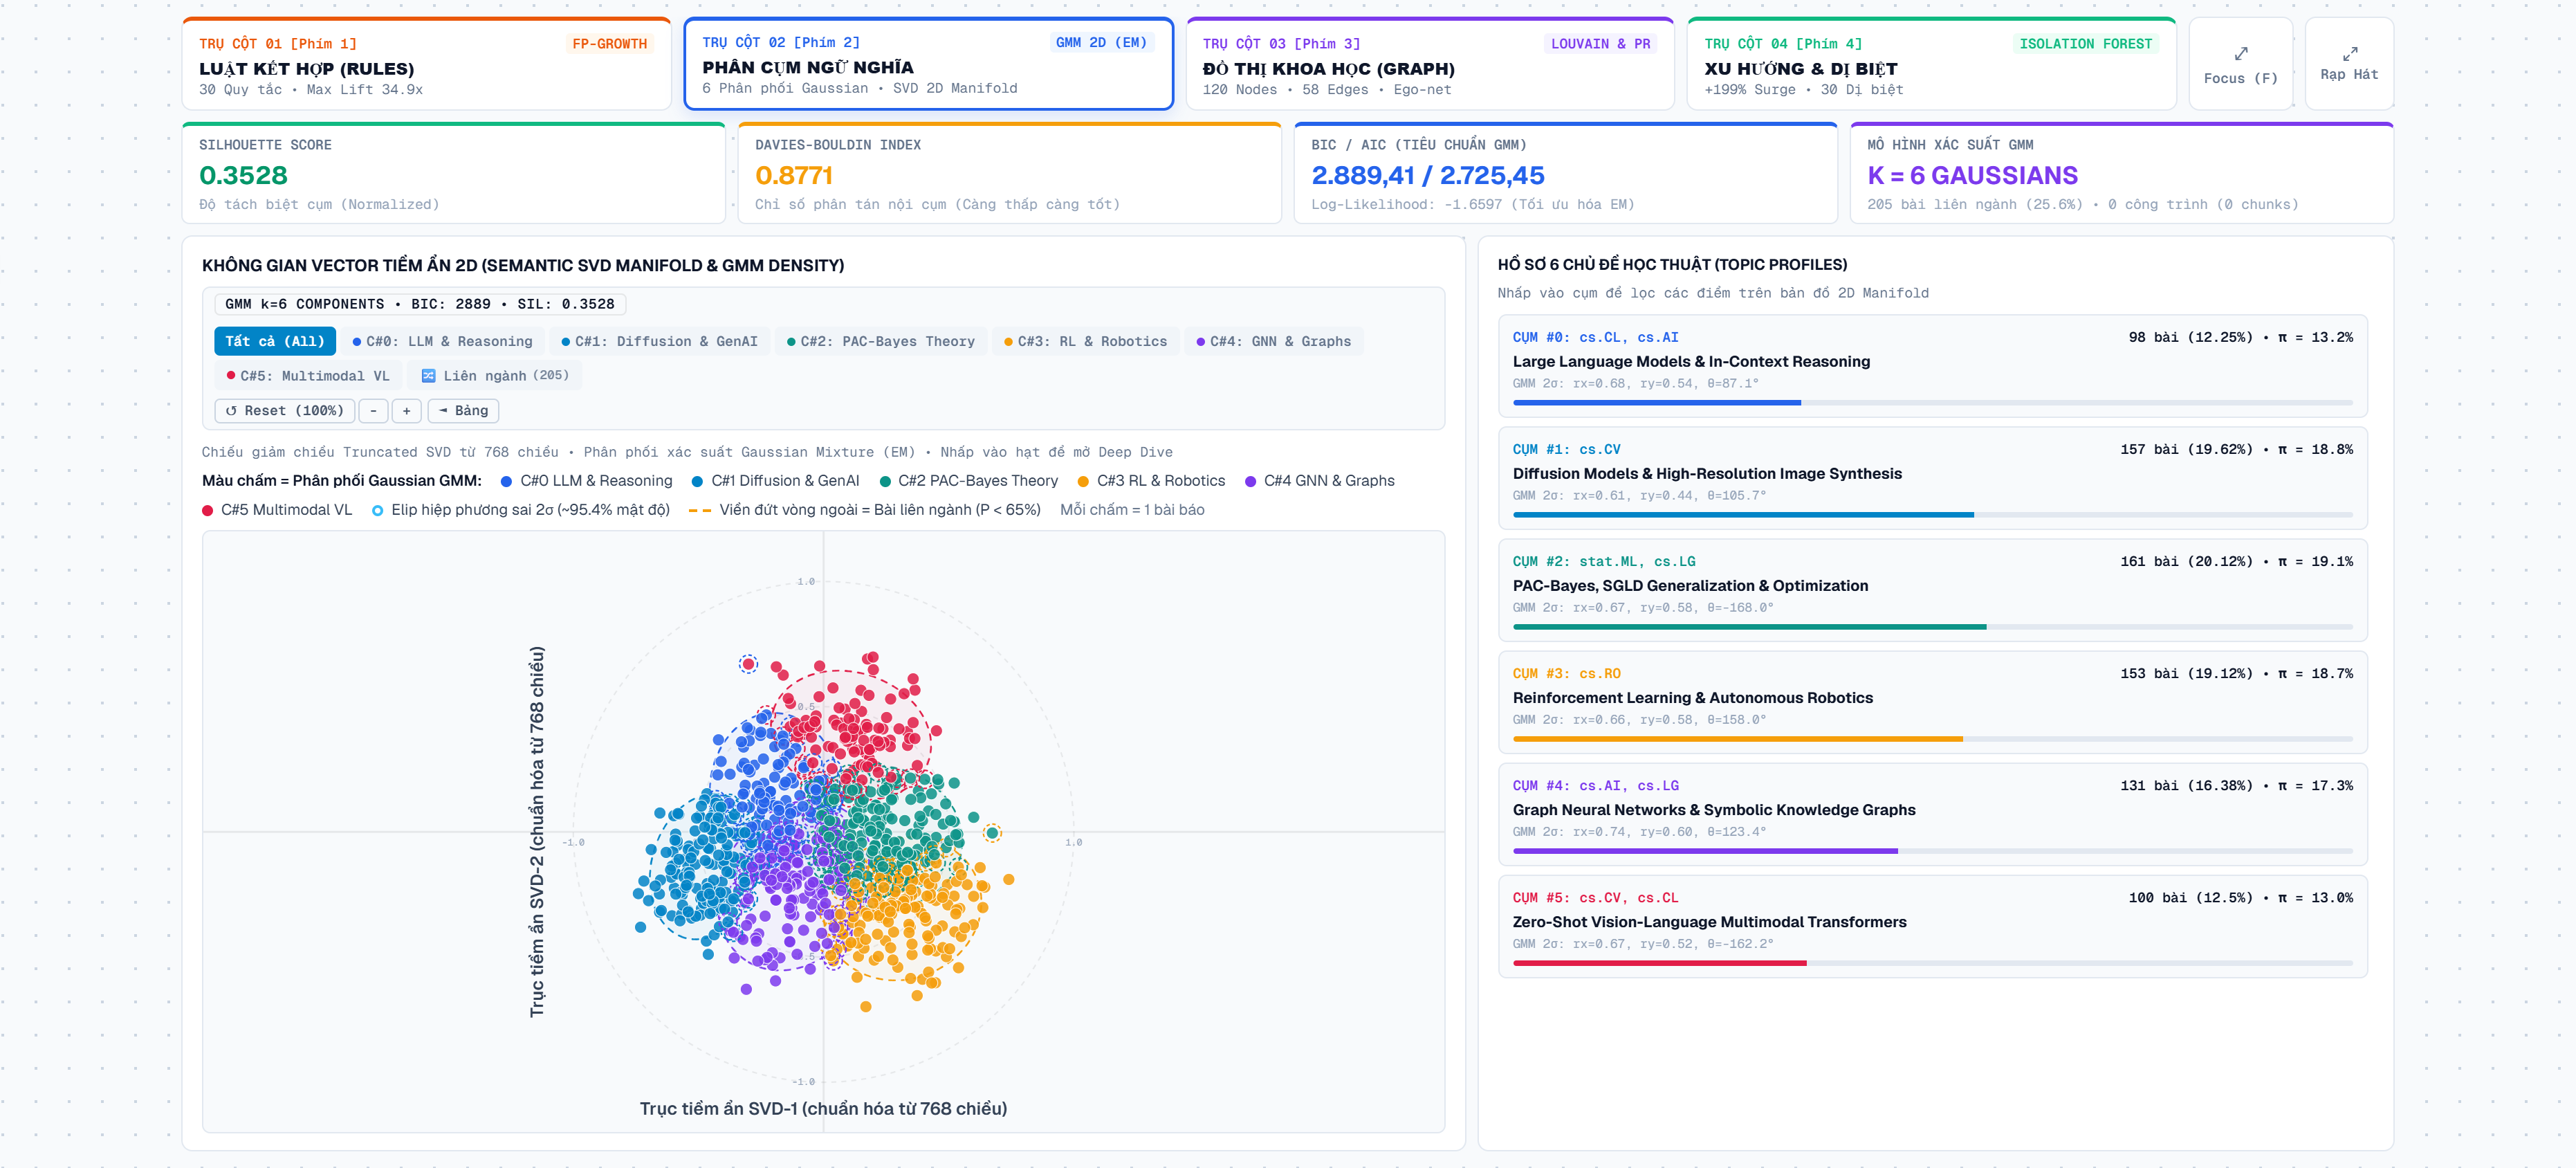
\includegraphics[width=\linewidth,height=0.68\textheight,keepaspectratio]{figures/captured_20261123_082337/06_gmm_clusters.png}
\caption[Giao diện kết quả GMM của snapshot 800 mẫu]{Giao diện kết quả GMM của snapshot 800 mẫu}
\label{fig:gmm_capture}
\ReportNote{Nguồn: Giao diện phân cụm Gaussian Mixture Model ($K=6$) trên không gian chiếu PCA 2D từ artifact \path{gold/mining/clusters.json}.}
\end{figure}
\FloatBarrier

\section{Trụ Cột 3: Khai Phá Mạng Lưới Khoa Học và Đồ Thị Trích Dẫn}

\subsection{Mô Hình Đồ Thị và Trọng Số Phân Số}
Hệ thống dựng đồ thị có hướng $G=(V,E)$ với cạnh từ bài trích dẫn tới bài được trích dẫn khi có \path{silver/citations.parquet} và metadata truy cập được. Khi không có tệp citation, code chuyển sang đồ thị đồng tác giả vô hướng. Artifact local hiện có là nhánh đồng tác giả, không xác nhận quy mô đồ thị citation live.

Khi xét trên góc độ mạng lưới đồng tác giả (Co-authorship Network) gồm 35,117 tác giả và 130,082 cạnh hợp tác, để ngăn chặn hiện tượng bùng nổ trọng số do các bài báo có danh sách tác giả khổng lồ (hàng trăm tác giả trong một dự án lớn), hệ thống áp dụng kỹ thuật \textbf{Trọng số phân số (Fractional Weighting)}:
\begin{equation}
  W(u, v) = \sum_{p \in P_{uv}} \frac{1}{N_p - 1}
\end{equation}
Trong đó $N_p$ là tổng số tác giả của bài báo $p$. Nếu hai tác giả là đồng tác giả duy nhất của bài báo ($N_p = 2$), trọng số là $1.0$; nếu bài báo có 100 tác giả, trọng số mỗi cặp liên kết chỉ là $\frac{1}{99} \approx 0.0101$.

\subsection{PageRank trên Đồ Thị Bài Báo và Đồng Tác Giả}
PageRank được trình bày theo mô hình bước đi ngẫu nhiên~\cite{page1999pagerank}.
Với hệ số suy giảm $\alpha=0.85$, bước chuyển từ $v$ sang $u$ được xác định bởi trọng số cạnh chuẩn hóa. Đối với đỉnh có cạnh đi ra, phần đóng góp vào PageRank có dạng:
\begin{equation}
  PR(u) = \frac{1 - \alpha}{|V|} + \alpha \sum_{v \in \mathcal{N}_{\text{in}}(u)} PR(v)\frac{w_{vu}}{\sum_z w_{vz}}
\end{equation}
NetworkX xử lý thêm đỉnh không có cạnh đi ra bằng phân phối chuyển tiếp mặc định. Với citation, nút là bài báo và cạnh biểu diễn trích dẫn; khi cạnh có cùng trọng số, mẫu số trở thành bậc ra. Với đồng tác giả, nút là tên tác giả và bước chuyển dùng trọng số hợp tác phân số trên đồ thị vô hướng. Vì vậy điểm cao của một tác giả phản ánh vị trí trong mạng hợp tác quan sát, không phải số trích dẫn hoặc độ ảnh hưởng đã được xác nhận của từng bài.

\subsection{Phát Hiện Cộng Đồng Nghiên Cứu (Louvain Modularity)}
Louvain tối ưu cấu trúc cộng đồng theo modularity~\cite{blondel2008fast}.
Thuật toán Louvain phân rã đồ thị thành các cộng đồng học thuật gắn kết chặt chẽ bằng cách tối ưu hóa hàm độ đo Modularity $Q$:
\begin{equation}
  Q = \frac{1}{2m} \sum_{i, j} \left[ A_{ij} - \frac{k_i k_j}{2m} \right] \delta(c_i, c_j)
\end{equation}
Trong đó $A_{ij}$ là trọng số cạnh, $k_i$ là tổng bậc trọng số của đỉnh $i$, $m$ là tổng trọng số cạnh của toàn mạng lưới, và $\delta(c_i, c_j) = 1$ khi đỉnh $i, j$ thuộc cùng cộng đồng. Thuật toán phát hiện được \textbf{3,740 cộng đồng} trong artifact đồng tác giả lịch sử. Với nhánh citation, Louvain chạy trên đồ thị đã chuyển vô hướng, còn PageRank chạy trên đồ thị có hướng.

Bảng~\ref{tab:graph_influencers} trình bày danh sách các tác giả có PageRank cao trong snapshot đồng tác giả; không ghép điểm bài landmark từ một lần chạy khác.

\begin{table}[!htbp]
\centering
\footnotesize
\setlength{\tabcolsep}{3pt}
\caption[Cấu trúc mạng lưới khoa học chế độ kép và Top nút uy tín PageRank]{Cấu trúc mạng lưới khoa học chế độ kép (Trích dẫn có hướng vs Đồng tác giả) và Top nút uy tín PageRank}
\label{tab:graph_influencers}
\begin{tabularx}{\linewidth}{|>{\raggedright\arraybackslash}p{28mm}|>{\centering\arraybackslash}p{14mm}|>{\centering\arraybackslash}p{15mm}|>{\centering\arraybackslash}p{16mm}|L|>{\raggedright\arraybackslash}p{34mm}|}
\hline
\textbf{Chế độ đồ thị} & \textbf{Nút ($|V|$)} & \textbf{Cạnh ($|E|$)} & \textbf{Cộng đồng} & \textbf{Nút uy tín tiêu biểu} & \textbf{PageRank \& Chỉ số chi tiết} \\ \hline
\textbf{Trích dẫn Có hướng} (hạng 1) & 8,892 & 86,295 & 92 & Vaswani et al. (\textit{Attention Is All You Need}~\cite{vaswani2017attention}) & \textbf{0.012632}; \path{in_degree} = 1,213; \path{cites} = 26,678 \\ \hline
\textbf{Trích dẫn Có hướng} (hạng 2) & 8,892 & 86,295 & 92 & Matthew E. Peters et al. (\textit{ELMo}) & \textbf{0.008603}; \path{in_degree} = 900; \path{cites} = 12,264 \\ \hline
\textbf{Trích dẫn Có hướng} (hạng 3) & 8,892 & 86,295 & 92 & Jakub\r{u}v, Jan et al. (\textit{Exploiting GenAI...}) & \textbf{0.007782}; \path{in_degree} = 1,145; \path{cites} = 78,459 \\ \hline
\textbf{Mạng Đồng tác giả} (snapshot cục bộ) & 35,117 & 130,082 & 3,740 & Yang Liu (hạng 1) / Hao Chen (hạng 2) & 0.000509 (\path{deg}=237, 38 bài) / 0.000463 (\path{deg}=189, 32 bài) \\ \hline
\textbf{Chỉ số mở rộng} (\path{citation_metrics.parquet}) & 29,523 tác giả & 10,000 bài nền & -- & Từ điển PageRank phục vụ thí nghiệm \texttt{EXP-04} & Kết hợp đồ thị bài báo và tác giả (Chương~\ref{chap:evaluation}) \\ \hline
\end{tabularx}
\ReportNote{Nguồn: \path{data/gold/mining/graph_coauthorship.json} (mật độ \path{density = 0.001092}, 29,911 bài lập chỉ mục), snapshot mạng đồng tác giả 35,117 tác giả, và \path{data/gold/graphs/citation_metrics.parquet}. Trong lần chạy sản xuất 04/11/2026 (\texttt{SNAP-06A}), \texttt{ScientificGraphMiner} tiêu tốn 116.39 giây (49.6\% tổng thời gian 234.57 giây).}
\end{table}


\subsection{Tích Hợp vào RAG: Cơ Chế PageRank Authority Multiplier}
\label{sec:authority_multiplier}
Hệ thống đưa điểm PageRank chuẩn hóa vào thuật toán xếp hạng tài liệu RAG trong \path{backend/app/services/retrieval_service.py}:
\begin{equation}
  \text{Score}_{\text{final}}(d) = \min\!\left(0.9999,\,\text{Score}_{\text{RRF}}(d)\left[1+\beta\min(1, PR_{\mathrm{match}}/PR_{\max})\right]\right)
\end{equation}
Ở hybrid mode, điểm RRF được ánh xạ sang khoảng 0.70--0.95 trước phép nhân trên. Nhánh tạo ứng viên đã áp dụng authority vào điểm dense trước khi lập thứ hạng, rồi hybrid áp dụng tiếp hệ số vào điểm fusion; vì vậy phải xem xét toàn bộ thứ tự xử lý khi làm ablation. Với $\beta=0.25$, mỗi phép nhân có hệ số tối đa 1.25; điểm hiển thị cuối bị chặn ở 0.9999, không phải xác suất câu trả lời đúng. Backend khớp tên tác giả đoạn trích với trường author trong danh sách influencer và chuẩn hóa theo PR lớn nhất đã nạp. Vì thế cơ chế này không phải lookup PageRank trực tiếp theo paper ID; không bảo đảm mọi landmark đều được ưu tiên đúng.

\section{Trụ Cột 4: Động Lượng Xu Hướng và Bản Đồ Dị Biệt (Trends \& Anomalies)}

\subsection{Vận Tốc Xu Hướng Chuẩn Hóa Thị Phần ($\Delta\text{Share}$ Momentum)}
Dữ liệu được gom theo tháng có quan sát, lấy ba tháng quan sát mới nhất so với ba tháng quan sát trước đó. Với chuyên ngành $c$, đặt $s_r(c)=N_r(c)/\max(1,\sum_c N_r(c))$ và $s_p(c)=N_p(c)/\max(1,\sum_c N_p(c))$. Động lượng được tính như sau:
\begin{equation}
g(c)=100\frac{s_r(c)-s_p(c)}{s_p(c)},\qquad \Delta s(c)=100(s_r(c)-s_p(c)).
\end{equation}
Nếu $s_p=0$, $g=100$ khi $s_r>0$, ngược lại bằng 0. Nhãn SURGING khi $g>15$ hoặc $\Delta s>1.5$; DECLINING khi $g<-15$ hoặc $\Delta s<-1.5$; còn lại STABLE. Chỉ các ngành có ít nhất 40 bài được xét. Đây là thay đổi thị phần trong tập quan sát, không phải tốc độ tăng của toàn bộ cộng đồng khoa học.

Artifact local cũ còn nhãn ACCELERATING và tỷ lệ tăng theo số lượng thô; không dùng các tỷ lệ đó làm kết quả của công thức thị phần hiện tại.

\subsection{Rừng Cô Lập (Isolation Forest) với Chuẩn Hóa $\log(1+x)$}
Để phát hiện các bài báo dị biệt về mặt cấu trúc tài liệu, hệ thống xây dựng vector 5 đặc trưng:
\begin{equation}
  \mathbf{x} = [\text{total\_math\_count}, \text{total\_words}, \text{total\_sections}, \text{author\_count}, \text{category\_count}]
\end{equation}
Các phân vị và cực trị EDA cho thấy chênh lệch lớn ở số từ và công thức. Hệ thống dùng phép biến đổi sau để nén khoảng giá trị và giảm ảnh hưởng của cực trị; chưa thực hiện kiểm định phân phối power law:
\begin{equation}
  \mathbf{x}_{\text{log}} = \log(1 + \mathbf{x})
\end{equation}
Isolation Forest~\cite{liu2008isolation} trong hệ thống xây dựng 100 cây cô lập ngẫu nhiên với tham số đặt ngưỡng $\text{contamination} = 0.02$. Điểm dị biệt được tính bằng:
\begin{equation}
  s(x, n) = 2^{-\frac{\mathbb{E}(h(x))}{c(n)}}
\end{equation}
Trong đó $h(x)$ là độ sâu của đường dẫn từ gốc đến lá cô lập mẫu $x$, và $c(n) = 2H_{n-1} - \frac{2(n-1)}{n}$ là chiều dài đường dẫn trung bình của cây tìm kiếm nhị phân không thành công, với $H_{n-1}$ là số điều hòa. Đây là điểm lý thuyết; trường \texttt{anomaly\_score} trong artifact dùng \texttt{score\_samples} của scikit-learn, có giá trị âm và thấp hơn biểu thị dị biệt hơn.

Bảng~\ref{tab:anomalies} tổng hợp danh sách các bài báo ngoại lai cấu trúc tiêu biểu phát hiện được trong kho dữ liệu.

\begin{table}[!htbp]
\centering
\footnotesize
\setlength{\tabcolsep}{3pt}
\caption[Kết quả động lượng thị phần và bất thường Isolation Forest]{Kết quả động lượng thị phần (\texorpdfstring{$\Delta\text{Share}$}{Delta Share}) và các bài báo bất thường cấu trúc tiêu biểu (\texttt{trends\_anomalies.json})}
\label{tab:anomalies}
\begin{tabularx}{\linewidth}{|>{\raggedright\arraybackslash}p{24mm}|>{\raggedright\arraybackslash}p{22mm}|>{\centering\arraybackslash}p{24mm}|L|>{\raggedright\arraybackslash}p{34mm}|}
\hline
\textbf{Mã / Ngành} & \textbf{Loại kết quả} & \textbf{Giá trị định lượng} & \textbf{Đặc trưng nổi bật} & \textbf{Trạng thái / Nhãn lý giải} \\ \hline
\path{cs.CV} & Động lượng & \texttt{growth = +123.43\%} & \path{recent = 722}, \path{prev = 6}, \path{all = 3,021} & \texttt{SURGING} \\ \hline
\path{cs.AI} & Động lượng & \texttt{growth = +198.94\%} & \path{recent = 161}, \path{prev = 1}, \path{all = 625} & \texttt{SURGING} \\ \hline
\path{cs.CL} & Động lượng & \texttt{growth = +69.89\%} & \path{recent = 366}, \path{prev = 4}, \path{all = 1,858} & \texttt{SURGING} \\ \hline
\path{cs.LG} & Động lượng & \texttt{growth = +38.64\%} & \path{recent = 672}, \path{prev = 9}, \path{all = 3,093} & \texttt{SURGING} \\ \hline
\path{cs.RO} & Động lượng & \texttt{growth = -81.43\%} & \path{recent = 160}, \path{prev = 16}, \path{all = 879} & \texttt{DECLINING} \\ \hline
\path{cs.IR} & Động lượng & \texttt{growth = -3.45\%} & \path{recent = 52}, \path{prev = 1}, \path{all = 310} & \texttt{STABLE} \\ \hline
\path{arXiv:2206.08756} & Ngoại lai IF (\#1) & \path{score = -0.7035} & 1,600 công thức, 15,279 từ, 6 nhãn ngành & Math-Heavy + Extreme Multidisciplinary \\ \hline
\path{arXiv:2501.05498} & Ngoại lai IF (\#2) & \path{score = -0.6906} & 5,470 công thức, 74,303 từ & Extreme Math + Mega-Survey Monograph \\ \hline
\path{arXiv:2401.13216} & Ngoại lai IF (\#3) & \path{score = -0.6865} & 3,732 công thức, 26,576 từ, 4 nhãn ngành & Math-Heavy + Mega-Survey + 4 Categories \\ \hline
\path{arXiv:2411.15221} & Ngoại lai đa tác giả & \path{score = -0.6826} & 144 đồng tác giả, 24,057 từ, 20 công thức & Hyper-Authorship Collaboration \\ \hline
\end{tabularx}
\ReportNote{Nguồn: \path{data/gold/mining/trends_anomalies.json} (lát cắt cục bộ 29,911 bài, 260 ngoại lai, 26 chuyên ngành). Trên lần chạy sản xuất 04/11/2026 (\texttt{SNAP-06A}), \texttt{TrendAnomalyMiner} xử lý toàn bộ 71,927 bài trong 2.89 giây, phát hiện 1,000 ngoại lai hàng đầu (\path{contamination = 0.02}) và theo dõi 48 chuyên ngành đạt ngưỡng \path{all_time >= 40}.}
\end{table}


\begin{calloutbox}{Phạm vi Ứng dụng Dị biệt}
Trong phiên chạy ngày 04/11/2026 trên 71,927 bài (\path{logs/run/backend.log}, 2.89 giây), Isolation Forest (\texttt{contamination=0.020}) gắn nhãn \textbf{1,000 bài báo dị biệt cấu trúc} (giới hạn \texttt{top\_anomalies=1000}) và đánh giá \textbf{48 nhánh xu hướng}. Con số 2\% là tham số đặt trước của mô hình, chưa có ground truth kiểm chứng độc lập bằng đánh giá chuyên gia. Chunker được áp dụng chung, chưa có nhánh kích hoạt hierarchical sub-chunking từ nhãn Isolation Forest.
\end{calloutbox}

\FloatBarrier
\section{Liên Hệ Giữa Khai Phá Dữ Liệu và Pipeline RAG}
\label{sec:mining_rag_integration}

\subsection{Lý Do Thiết Kế và Phạm Vi Tích Hợp Mining}
Các đầu ra mining phục vụ những nhiệm vụ khác nhau nên mức tích hợp với retrieval cũng khác nhau. Về mặt thiết kế, lọc cứng theo nhãn cụm có nguy cơ loại tài liệu liên ngành, còn mở rộng query có thể thêm cả tín hiệu hữu ích và nhiễu. Hai cách can thiệp này không đồng nhất. Chưa có phép đo recall trước/sau hoặc ablation được lưu để xác nhận chúng đã gây suy giảm trong hệ thống.

Trong implementation hiện tại, các vai trò được phân biệt như sau:
\begin{enumerate}[label=\textbf{\arabic*.}]
\item \textbf{Tín hiệu xếp hạng}: PageRank khớp theo tác giả điều chỉnh điểm retrieval/fusion trước khi chọn tập ứng viên cho cross-encoder. Phép nhân không sửa trực tiếp vector query nhưng có thể thay đổi thứ hạng và tập đoạn được chọn. Tác động lên độ phủ và chất lượng cần được đo; điểm PageRank đồng tác giả cũng không phải chứng nhận ảnh hưởng học thuật của từng bài.
\item \textbf{Khám phá corpus và annotation}: FP-Growth trả gợi ý luật trong response; clustering và Isolation Forest cung cấp bản đồ ngữ nghĩa cùng nhãn dị biệt cấu trúc cho dashboard. Các đầu ra này chưa được đưa vào prompt như một nguồn ngữ cảnh mining riêng. Nhãn dị biệt cấu trúc không được đồng nhất với tính mới học thuật.
\end{enumerate}

Prompt có dẫn nguồn và chỉ dẫn từ chối khi thiếu chứng cứ là cơ chế riêng ở bước sinh câu trả lời. Không coi việc có dashboard hoặc annotation là bằng chứng các thuật toán mining đã hoạt động như guardrails cho LLM. Phân tách vai trò giúp xác định đúng các cấu hình cần đối chứng khi đánh giá tích hợp.

\subsection{Chu Trình Xử Lý Truy Vấn End-to-End}
Quy trình phối hợp giữa các thành phần được thực thi theo 5 bước:
\begin{enumerate}[label=\alph*)]
\item Nhúng query gốc bằng Nomic. Luật FP-Growth sinh annotation gợi ý danh mục liên đới, không làm biến dạng vector query gốc.
\item Qdrant lấy pool thô theo $\min(\max(2k,25),40)$ với $k$ là số kết quả retrieval được yêu cầu; hydrate text và metadata từ Silver chunks. Có nhánh tra trực tiếp paper ID hoặc khớp title.
\item Trong hybrid mode, xếp lại cùng pool bằng điểm từ vựng heuristic (phrase, acronym, title, section), hòa trộn RRF với hằng số 60 và nhân hệ số uy tín PageRank theo công thức xếp hạng.
\item Chat mặc định yêu cầu 8 ứng viên từ retrieval, sau đó Cross-Encoder lấy Top-5; các giá trị có thể đổi bằng cấu hình/request.
\item LLM nhận các đoạn đã chọn và prompt yêu cầu dẫn nguồn, bảo toàn LaTeX, từ chối khi thiếu chứng cứ; temperature mặc định của ChatRequest là 0.1.
\end{enumerate}
\begin{figure}[htbp]
\centering
\DrawRagPipelineDiagram
\caption[Luồng truy xuất và sinh câu trả lời RAG]{Luồng truy xuất và sinh câu trả lời RAG}
\label{fig:rag_pipeline_flow}
\end{figure}
Clustering và anomaly phục vụ dashboard, chưa điều hướng trực tiếp retrieval. Các guardrail giảm rủi ro sai lệch nhưng không bảo đảm loại bỏ ảo giác.

\FloatBarrier
\Needspace{8\baselineskip}
\section{Tham Số Cấu Hình Hệ Thống}
\begingroup
\small
\setlength{\tabcolsep}{4pt}
\setlength{\LTpre}{4pt}
\setlength{\LTpost}{6pt}
\begin{longtable}{|>{\raggedright\arraybackslash}p{27mm}|>{\raggedright\arraybackslash}p{40mm}|>{\centering\arraybackslash}p{15mm}|>{\raggedright\arraybackslash}p{61mm}|}
\caption[Tham số cấu hình hệ thống]{Tham số cấu hình mặc định của hệ thống}
\label{tab:hyperparameters}\\
\hline
\textbf{Phân hệ} & \textbf{Tham số} & \textbf{Giá trị} & \textbf{Ý nghĩa} \\ \hline
\endfirsthead
\multicolumn{4}{l}{\small Bảng \thetable{} (tiếp theo)}\\
\hline
\textbf{Phân hệ} & \textbf{Tham số} & \textbf{Giá trị} & \textbf{Ý nghĩa} \\ \hline
\endhead
\hline
\multicolumn{4}{r}{\small Còn tiếp ở trang sau}\\
\endfoot
\hline
\endlastfoot
FP-Growth & \path{min_support} & 0.02 & Mặc định; snapshot cũ dùng 0.015 \\ \hline
FP-Growth & \path{min_lift} & 1.20 & Ngưỡng lift ban đầu; có fallback \\ \hline
FP-Growth & \path{top_k} & 50 & Giới hạn số luật trả về \\ \hline
FP-Growth & \path{min_abs_transactions} & 25 & Số giao dịch hỗ trợ tuyệt đối tối thiểu \\ \hline
Clustering & \path{vector_dim} & 768 & Số chiều embedding Nomic \\ \hline
Clustering & \path{n_clusters} & 6 & Mặc định KMeans và GMM \\ \hline
Clustering & \path{pca_components} & 2 & Chiếu 2D để hiển thị và fit GMM \\ \hline
Clustering & \path{dbscan_eps / min_samples} & 0.28 / 10 & DBSCAN dùng khoảng cách cosine trên mẫu \\ \hline
Graph & \path{pagerank_alpha} & 0.85 & Hệ số suy giảm PageRank \\ \hline
Graph & \path{authority_beta} & 0.25 & Hệ số uy tín theo tác giả; tối đa +25\% \\ \hline
Anomalies & \path{contamination} & 0.02 & Tỷ lệ dị biệt cấu trúc đặt trước \\ \hline
Anomalies & \path{n_estimators} & 100 & Số cây trong Isolation Forest \\ \hline
RAG & \path{RERANKER_CANDIDATE_K} & 8 & Ứng viên retrieval trả cho reranker; pool Qdrant mặc định 25 \\ \hline
RAG & \path{RERANKER_TOP_K} & 5 & Số đoạn giữ lại; request có thể ghi đè \\ \hline
RAG & \path{rrf_constant} & 60 & Hằng số làm mịn RRF \\ \hline
Chat & \path{temperature} & 0.1 & Mặc định của ChatRequest \\ \hline
\end{longtable}
\ReportNote{Nguồn: các module mining, cấu hình backend và ChatRequest tại commit \texttt{e828310}. Giá trị trong môi trường chạy hoặc request có thể ghi đè các mặc định cấu hình.}
\endgroup



Bốn đầu ra mining cung cấp các góc nhìn bổ trợ, nhưng việc xuất được artifact chưa xác nhận lợi ích truy xuất. Chương~\ref{chap:evaluation} lần lượt xem xét tính diễn giải của mining, chất lượng RAG lịch sử và độ trễ phần cứng. Những thay đổi cùng lúc trong pipeline được tách khỏi kết luận về tác động riêng của từng thuật toán.

\clearpage

% Chương 5: Đánh giá Thực nghiệm Toàn diện & Phân tích Benchmark (Evaluation)
\chapter{Đánh Giá Thực Nghiệm Hệ Thống (Evaluation)}
\label{chap:evaluation}
\section{Phạm Vi Chứng Cứ và Khác Biệt Phiên Bản}
Đánh giá cần trả lời hai vấn đề khác nhau: các đầu ra mining mô tả được điều gì về corpus và pipeline RAG đạt chất lượng/độ trễ ra sao. Source xác nhận chức năng tại commit \texttt{e828310} (05/11/2026), còn các kết quả dưới đây được tổng hợp từ chứng cứ lưu trữ. Ba nhóm nguồn chính gồm:
\begin{itemize}
\item Artifact local trong \path{data/gold/mining/}, được manifest 04/10/2026 tham chiếu, còn ghi nguồn LanceDB/local. Đây là nguồn thống kê mô tả và kết quả mining lịch sử.
\item Báo cáo DeepEval 05/10/2026, ghi commit \texttt{6cb1c52}, dùng LanceDB và hơn 143 nghìn chunk trên Cloudflare R2. Đây là nguồn so sánh chất lượng RAG lịch sử.
\item Báo cáo phần cứng 19/10/2026 gồm benchmark Qdrant độc lập và benchmark end-to-end với LLM trên RTX 4060/CUDA. Hai kịch bản có phạm vi và cách đo khác nhau.
\end{itemize}

Hai giai đoạn được liên hệ ở mức ý tưởng thiết kế, không mặc nhiên tương đương về hiệu quả. Benchmark LanceDB là chứng cứ thăm dò cho cấu hình và tập câu hỏi đã đo; một số metric tăng và một số giảm, chưa xác nhận ưu thế tổng quát hoặc tính đúng đắn của toàn pipeline. Qdrant và Silver chunks thay đổi cách lập chỉ mục, lấy nội dung và quản lý dữ liệu. Khả năng mở rộng, thông lượng đồng thời và độ trễ hydrate của kiến trúc mới cần phép đo tải cùng cấu hình được kiểm soát; chưa có kết quả để khẳng định đạt quy mô công nghiệp hoặc giữ nguyên hiệu quả truy xuất sau chuyển đổi.

Quy ước chung là giữ kết quả theo nguồn, phân biệt điều quan sát được với hiệu quả chưa được xác nhận. Không nối các nguồn thành một lần chạy của phiên bản mới. Các ảnh phục vụ minh họa có phạm vi riêng ở Bảng~\ref{tab:snapshot_sources}; chi tiết truy vết nằm ở phụ lục.

\section{Đánh Giá Định Lượng Các Artifact Mining Lịch Sử}
\begin{enumerate}
\item \textbf{EDA}: 10,000 bài, 9,015 bài mang nhãn làm giàu, 2,220,938 công thức và 47,782,707 từ. Các số này xác nhận quy mô được ghi trong artifact. Để đánh giá chất lượng cần kiểm tra thêm metadata thiếu, lỗi parser và độ đúng của công thức trên mẫu tài liệu.
\item \textbf{FP-Growth}: 282 giao dịch, 38 itemset, 22 luật; manifest ghi 0.49 giây. Các ví dụ có số giao dịch hỗ trợ nhỏ như phân tích ở Chương~\ref{chap:modeling}. Artifact còn luật đối xứng và có lift dưới threshold khai báo, nên chưa dùng để xác nhận hiệu quả khử đối xứng của code mới hoặc lợi ích query expansion.
\item \textbf{Clustering}: snapshot 5,000 mẫu, 768 chiều, $K=6$, có Silhouette 0.0210, Davies--Bouldin 5.3739 và Calinski--Harabasz 88.0. Silhouette cho thấy mức tách biệt thấp theo metric đã dùng. DBSCAN cho một cụm, noise ratio 0.0; chưa có cơ sở gán nhãn chủ đề chính xác hoặc kết luận đã phát hiện các trường phái. Runtime 0.48 giây thuộc module cũ, không bao gồm toàn bộ pipeline PCA/GMM hiện tại.
\item \textbf{Graph}: mạng đồng tác giả ghi 35,117 tác giả, 130,082 cạnh, 3,740 cộng đồng và 3,516 thành phần liên thông; runtime 72.2 giây. Số thành phần liên thông cùng số cộng đồng cho thấy cần khảo sát kích thước và mức phân mảnh trước khi diễn giải từng cộng đồng. Thứ hạng ở đây là của tác giả trong mạng hợp tác, không phải đánh giá landmark bằng citation.
\item \textbf{Dị biệt và xu hướng}: summary ghi 200 điểm được gắn nhãn, danh sách xuất có 30 bản ghi, còn manifest đếm 30 và ghi 0.14 giây. Tỷ lệ 2\% gắn với contamination đặt trước; cần chuyên gia hoặc tập nhãn để đánh giá khả năng phát hiện dị biệt có ý nghĩa. Trend cũ dùng nhãn ACCELERATING và số lượng thô, chưa đánh giá công thức thị phần mới.
\end{enumerate}

Tổng runtime manifest là 73.33 giây; riêng graph chiếm phần lớn với 72.2 giây. Đây là gợi ý ưu tiên đo lại graph khi khảo sát chi phí mining, không phải kết luận về nút thắt của phiên bản mới. Toàn bộ kết quả trên hỗ trợ mô tả corpus và chỉ ra vấn đề dữ liệu; số artifact hoặc tốc độ xuất artifact không tự xác nhận giá trị học thuật hay tác động tới RAG.

\section{Benchmark DeepEval 2.x trên Kiến Trúc LanceDB Lịch Sử}
Nguồn \path{docs/benchmarks/RAG_EVALUATION_REPORT_21_SAMPLES.md} so sánh dense baseline với pipeline nâng cao trên 21 câu hỏi được tuyển chọn (gold-001 đến gold-021), dùng Qwen2.5-7B-Instruct làm LLM judge. Baseline dùng Top-5; pipeline nâng cao dùng pool 15 cùng reranker, fusion và guardrail. Đây là so sánh nhiều thay đổi đồng thời; cấu hình khác với backend hiện tại lấy mặc định 8 ứng viên trước reranking.

Các metric đánh giá những khía cạnh khác nhau: Contextual Precision xem thứ hạng ngữ cảnh hữu ích, Contextual Recall xem độ phủ so với câu trả lời kỳ vọng, Answer Relevancy xem mức liên quan tới câu hỏi, còn Faithfulness xem mức được ngữ cảnh hỗ trợ. Score trung bình và tỷ lệ vượt ngưỡng cần được đọc riêng; metric dùng LLM judge chưa thay thế đánh giá chuyên gia.
\begin{table}[htbp]
  \centering
  \small
  \caption[Kết quả DeepEval lịch sử trên LanceDB ngày 05/10/2026]{Kết quả đánh giá DeepEval lịch sử trên kiến trúc LanceDB ngày 05/10/2026 (21 mẫu PoC)}
  \label{tab:rag_benchmark}
  \vspace{4pt}
  \setlength{\tabcolsep}{3.0pt}
  \begin{tabularx}{\linewidth}{|>{\raggedright\arraybackslash}p{28mm}|>{\centering\arraybackslash}p{15mm}|>{\centering\arraybackslash}p{22mm}|>{\centering\arraybackslash}p{16mm}|>{\centering\arraybackslash}p{23mm}|>{\centering\arraybackslash}p{16mm}|>{\centering\arraybackslash}X|}
    \hline
    \textbf{Chỉ số DeepEval} & \textbf{Baseline} & \textbf{Tỷ lệ đạt} & \textbf{Upgraded} & \textbf{Tỷ lệ đạt} & \textbf{Chênh $\Delta$} & \textbf{Tương đối} \\
    \hline
    \textbf{Context Precision} $\uparrow$ & 0.637 & 60.0\% (12/20) & \textbf{0.860} & \textbf{80.0\% (16/20)} & \textbf{+0.223} & \textbf{+35.0\%} \\
    \hline
    \textbf{Answer Relevancy} $\uparrow$ & 0.687 & 47.4\% (9/19) & \textbf{0.752} & \textbf{55.0\% (11/20)} & \textbf{+0.065} & \textbf{+9.4\%} \\
    \hline
    \textbf{Context Recall} $\uparrow$ & 0.950 & 95.0\% (19/20) & \textbf{1.000} & \textbf{100.0\% (19/19)} & \textbf{+0.050} & \textbf{+5.3\%} \\
    \hline
    \textbf{Faithfulness} $\uparrow$ & 0.668 & 50.0\% (8/16) & \textbf{0.699} & \textbf{52.9\% (9/17)} & \textbf{+0.031} & \textbf{+4.7\%} \\
    \hline
    \textbf{Citation Grounding} $\uparrow$ & 0.757 & 90.5\% (19/21) & \textbf{0.720} & \textbf{90.0\% (18/20)} & -0.037 & -4.9\% \\
    \hline
    \textbf{Context Relevancy} & 0.578 & 44.4\% (4/9) & 0.562 & 40.0\% (6/15) & -0.016 & Đánh đổi \\
    \hline
  \end{tabularx}
  \ReportNote{Nguồn: Thử nghiệm PoC lịch sử ngày 05/10/2026 (\path{docs/benchmarks/RAG_EVALUATION_REPORT_21_SAMPLES.md}, commit \texttt{6cb1c52}, kho LanceDB R2 gồm 143,523 đoạn văn) trên 21 truy vấn (\texttt{gold-001} đến \texttt{gold-021}) sử dụng giám khảo \texttt{Qwen2.5-7B-Instruct}. Đây là mốc thăm dò tiền đề cho việc tinh chỉnh Laya ở \texttt{EXP-05}.}
\end{table}


\subsection{Diễn Giải và Giới Hạn Đánh Giá}
\begin{itemize}
\item Contextual Precision tăng từ 0.637 lên 0.860 (+35.0\% tương đối), với 16/20 mẫu hợp lệ vượt ngưỡng ở pipeline nâng cao. Kết quả gợi ý cải thiện thứ hạng ngữ cảnh trong cấu hình đã đo; chưa có ablation để quy cho reranker, authority hoặc fusion riêng lẻ.
\item Contextual Recall 1.000 và pass 19/19 áp dụng cho mẫu tính được metric. Không dùng 19 mẫu này làm kết luận độ phủ cho toàn bộ 21 câu hoặc các câu hỏi ngoài tập tuyển chọn.
\item Answer Relevancy tăng từ 0.687 lên 0.752 (pass 11/20); Faithfulness đạt 0.699 và pass 9/17 (52.9\%). Kết quả cho thấy mức được ngữ cảnh hỗ trợ còn hạn chế trong cấu hình đã đo. Điểm aggregate chưa xác định nguyên nhân là retrieval thiếu đoạn, giới hạn context, lỗi trích xuất hay cách mô hình sinh sử dụng chứng cứ. Độ khó của công thức và suy luận nhiều bước chỉ là giả thuyết cần kiểm tra bằng phân tích từng câu hỏi và raw trace, không phải nguyên nhân đã được chứng minh.
\item Citation Grounding có score 0.720 và pass 18/20, nhưng score giảm từ 0.757. Contextual Relevancy cũng giảm 0.578 xuống 0.562. Vì vậy không thể mô tả kết quả là cải thiện đồng đều mọi mặt hoặc đã giải quyết ảo giác.
\end{itemize}

Số mẫu hợp lệ khác nhau theo metric và giữa hai pipeline làm phép so sánh chưa phải đối chứng cặp hoàn chỉnh. Báo cáo nguồn chưa cung cấp đủ raw traces để tái kiểm tra các trường hợp lỗi trong lần biên tập này; không có kiểm định ý nghĩa thống kê hoặc khoảng tin cậy được bổ sung. Kết quả được xem là chứng cứ thăm dò cho cấu hình lịch sử, chưa xác nhận hiệu quả tổng quát của hệ thống hiện tại.

\section{Đo Lường Phần Cứng Ngày 19/10/2026}
Nguồn \path{docs/benchmarks/PERFORMANCE_BENCHMARK_REPORT.md} ghi Windows 11, Python 3.12, RTX 4060 Laptop 8 GB và CUDA 12.4 cho benchmark LLM. Cần phân biệt hai phép đo:
\begin{enumerate}
\item \textbf{Truy vấn Qdrant độc lập}: Có 3 lượt warmup và 20 lượt đo cho mỗi scenario. Top-5 không lọc đạt mean 269.46 ms, median 268.10 ms; nguồn so sánh kết nối lạnh trên 1,000 ms với kết nối dùng pool. Đây chủ yếu là thay đổi cách kết nối và bối cảnh đo, không phải tác động riêng của CUDA lên máy chủ Qdrant.
\item \textbf{Pipeline RAG end-to-end}: Dùng retrieval Top-3 và LLM Qwen2.5-7B; nguồn ghi khoảng 1,660 ms cho phần retrieval trong phân rã này, TTFT 609.77 ms, sinh 50 token trong 1,079.43 ms và tổng 3,392.50 ms. Retrieval này không được thay bằng 269.46 ms từ phép đo độc lập để cộng thành tổng pipeline.
\end{enumerate}
\begin{table}[htbp]
  \centering
  \footnotesize
  \setlength{\tabcolsep}{3pt}
  \caption[Hồ sơ hiệu năng phần cứng RTX 4060 và pooling kết nối]{Hồ sơ hiệu năng phần cứng RTX 4060 và tối ưu hóa đường ống ngày 19/10/2026}
  \label{tab:latency_profile}
  \vspace{4pt}
  \begin{tabularx}{\linewidth}{|>{\raggedright\arraybackslash}p{34mm}|>{\centering\arraybackslash}p{26mm}|>{\centering\arraybackslash}p{26mm}|>{\centering\arraybackslash}p{21mm}|L|}
    \hline
    \textbf{Giai đoạn / Thông số đo} & \textbf{Trước tối ưu (Vulkan / Cold)} & \textbf{Sau tối ưu (CUDA / Pool)} & \textbf{Tăng tốc / Giới hạn} & \textbf{Ghi chú kỹ thuật} \\
    \hline
    \textbf{Qdrant độc lập (Top-5 / Top-50)} & $> 1,000$ ms (Cold TCP) & \textbf{269.46 $\pm$ 12.44 ms} (3.71 QPS) & Top-50: 258.80 ms (3.86 QPS) & HTTP Pooling (\texttt{requests.Session}); $p_{50}=268.10$, $p_{95}=291.50$ ms \\
    \hline
    \textbf{Nhúng câu hỏi (Query Embed)} & $\approx 350.0$ ms & \textbf{39.33 $\pm$ 21.64 ms} & \textbf{8.9$\times$ nhanh hơn} & Bi-Encoder 768-D trên GPU \\
    \hline
    \textbf{Ghép ngữ cảnh (Prompt)} & 5.0 ms & \textbf{0.04 $\pm$ 0.01 ms} & -- & Dựng chuỗi Prompt RAG \\
    \hline
    \textbf{Time To First Token (TTFT)} & 18,700 ms (18.7 s) & \textbf{609.77 $\pm$ 148.83 ms} & \textbf{30.7$\times$ nhanh hơn} & Hấp thụ Prompt Eval trên Tensor Cores \\
    \hline
    \textbf{Sinh 50 token tiếp theo} & 17,740 ms (17.7 s) & \textbf{1,079.43 $\pm$ 14.99 ms} & \textbf{16.4$\times$ nhanh hơn} & Giải mã tự hồi quy trên CUDA \\
    \hline
    \textbf{Tốc độ sinh (Throughput)} & 3.64 tok/s$^*$ & \textbf{46.33 $\pm$ 0.64 tok/s} & \textbf{12.7$\times$ nhanh hơn} & Vượt chuẩn đọc mượt thời gian thực \\
    \hline
    \textbf{Tổng RAG End-to-End (Top-3)} & 37,310 ms (37.31 s) & \textbf{3,392.50 $\pm$ 607.22 ms} & \textbf{$\approx 11.0\times$ nhanh hơn} & Gồm $\approx 1,660$ ms retrieval trong phép đo E2E \\
    \hline
    \textbf{Đỉnh VRAM \& Ổn định} & \path{VK_ERROR_DEVICE_LOST} & \textbf{$\approx 5.7$ GB / 8.0 GB} & Khử sập Vulkan & \path{LLM_CONTEXT_SIZE=4096}, \path{LLM_SEQUENCES=1} \\
    \hline
  \end{tabularx}
  \ReportNote{Nguồn: \path{docs/benchmarks/PERFORMANCE_BENCHMARK_REPORT.md} (19/10/2026) đo trên Windows 11, Python 3.12, NVIDIA GeForce RTX 4060 Laptop 8 GB, CUDA 12.4, \texttt{node-llama-cpp v3.15.5} và \texttt{Qwen-2.5-7B-Instruct Q4\_K\_M}. $^*$Nguồn gốc ghi 3.64 tok/s dù 50 token / 17.74 s tương ứng 2.82 tok/s; bảng giữ nguyên giá trị gốc để bảo đảm tính xác thực nguồn.}
\end{table}


Bảng~\ref{tab:latency_profile} tổng hợp số nguồn ghi cho các kịch bản, không phải một bảng phân rã có thể cộng mọi dòng. Với retrieval khoảng 1,660 ms, tổng các phần CUDA được nêu xấp xỉ 3,388.57 ms, gần tổng 3,392.50 ms; chênh lệch có thể gồm độ làm tròn hoặc phần chưa tách riêng, chưa được xác nhận bằng trace. Nếu dùng 269.46 ms của benchmark độc lập thì tổng chỉ 1,998.03 ms và không mô tả phép đo end-to-end.

Baseline còn một bất nhất: 50 token trong 17.74 giây tương ứng khoảng 2.82 tokens/s, khác 3.64 tokens/s được nguồn ghi. Bảng giữ nguyên hai giá trị theo nguồn, đánh dấu cần xác minh và không dùng chúng để khẳng định mức tăng tốc sinh token. Các tỷ số còn lại là so sánh mô tả giữa cấu hình lịch sử, không tách được tác động riêng của backend, context hoặc cách kết nối.

Code dùng \texttt{requests.Session()} và \texttt{HTTPAdapter} để tái sử dụng kết nối. Cấu hình phần cứng của nguồn là context 4096, sequences 1 và VRAM 5.7 GB/8 GB; backend hiện có mặc định \texttt{LLM\_CONTEXT\_WINDOW}=16384. Hai cấu hình phải được ghi riêng khi đo lại độ trễ và độ ổn định.

\section{Các Nghiên Cứu Điển Hình và Giới Hạn Nguồn}
\subsection{DPO (gold-003)}
Nguồn ghi Contextual Precision tăng từ 0.000 lên 1.000 sau nâng cấp. Đây là ví dụ về thay đổi thứ hạng ngữ cảnh, phù hợp với xu hướng aggregate; chưa đủ để chứng minh một thành phần cụ thể gây ra cải thiện hoặc mọi câu trả lời về DPO đều đúng.

\subsection{SVGD (gold-020)}
Case study ghi mô hình từ chối vì thiếu tài liệu về Stein Variational Gradient Descent, nhưng bảng diagnostic cùng nguồn ghi Faithfulness của gold-020 giảm từ 0.86 xuống 0.00. Do mâu thuẫn nội bộ, trường hợp này được giữ như điểm cần kiểm tra trace, không dùng làm minh chứng guardrail từ chối đúng.

\section{Kết Quả Đối Chiếu và Yêu Cầu Tái Lập}
Với câu hỏi về tổ chức dữ liệu, source xác nhận các bước fetch/embed, lưu Silver chunks và hydrate; cần kiểm tra vận hành để xác nhận tính đầy đủ cùng đồng bộ. Với câu hỏi về mining, artifact cho kết quả mô tả nhưng còn hạn chế về cỡ mẫu, nhãn và tính diễn giải. Với câu hỏi về RAG, benchmark lịch sử cho thấy một số metric tốt lên, đồng thời grounding còn hạn chế và chưa đo lại kiến trúc mới.

Phép đánh giá tiếp theo cần cố định commit, corpus, model và cấu hình; lưu raw traces, số mẫu lỗi và cặp câu hỏi chung. Ablation phải tách dense, lexical/RRF, authority và reranker; query expansion chỉ được đánh giá sau khi thực sự đưa vào retrieval. Kiểm tra công thức, nhãn dị biệt và cụm cần thêm đánh giá nội dung. Từ các giới hạn này, chương triển khai tập trung vào khả năng theo dõi trạng thái, đồng bộ Silver/Qdrant và xử lý lỗi thay vì suy ra độ sẵn sàng từ ảnh giao diện.

\clearpage

% Chương 6: Triển khai, Bảo mật & Vận hành Hệ thống (Deployment)
% ==============================================================================
% CHƯƠNG 6: TRIỂN KHAI VÀ VẬN HÀNH HỆ THỐNG (DEPLOYMENT)
% ==============================================================================

\chapter{Triển Khai và Vận Hành Hệ Thống (Deployment)}
\label{chap:deployment}

Kết quả đánh giá cho thấy cần phân biệt cấu hình phần mềm, phép đo lịch sử và trạng thái dịch vụ tại một thời điểm. Chương này mô tả các thành phần vận hành và cách kiểm tra chúng, đặc biệt là đường đi từ nội dung Silver tới kết quả Qdrant. Ảnh giao diện giúp nhận diện chức năng; độ sẵn sàng và chất lượng câu trả lời cần phép kiểm tra riêng.


\section{Kiến Trúc Vận Hành Phân Tán (Distributed Infrastructure)}

Hệ thống được thiết kế theo mô hình vi dịch vụ phân tán (\textit{Distributed Microservices Architecture}), sử dụng các dịch vụ hạ tầng độc lập; backend, frontend và worker có thể chạy ngoài container theo môi trường triển khai. Repository này không kèm toàn bộ Docker Compose của hạ tầng:

\begin{figure}[htbp]
  \centering
  \DrawSystemArchitecture
  \caption[Kiến trúc thu thập, lưu trữ và phục vụ RAG]{Kiến trúc thu thập, lưu trữ và phục vụ RAG}
  \ReportNote{Nguồn: Sơ đồ kiến trúc phân tầng tích hợp đường ống thu thập, lưu trữ Medallion Lakehouse và hệ thống phục vụ truy xuất RAG.}
  \label{fig:system_architecture}
\end{figure}

Các thành phần hạ tầng cốt lõi bao gồm:

\begin{enumerate}[label=\textbf{\arabic*.}]
  \item \textbf{Tầng Điều phối Tự động (Orchestration - Apache Airflow 2.10)}:
    Được cấu hình vận hành theo múi giờ chuẩn Việt Nam (\path{Asia/Ho_Chi_Minh - ICT}). Các DAG liên quan gồm:
    \begin{itemize}
      \item \texttt{dag\_tier1\_realtime\_stream}: Kích hoạt lúc 19:00 ICT hàng ngày quét RSS mới nhất.
      \item \texttt{dag\_tier2\_near\_past\_harvest}: Kích hoạt lúc 19:10 ICT hàng ngày, luân phiên CVF/arXiv theo ngân sách.
      \item \texttt{dag\_recompute\_mining}: Dùng cron 0 0 * * 0; giờ thực tế theo timezone Airflow vì DAG này chưa đặt timezone tường minh, gọi endpoint nội bộ \path{/api/mining/trigger} để tính toán lại toàn bộ EDA và 4 Trụ cột Khai phá trên dữ liệu mới tích lũy.
      \item \texttt{dag\_compact\_silver}: Chạy mỗi 3 giờ, gộp part của cả Silver papers và Silver chunks.
    \end{itemize}
  \item \textbf{Tầng Hàng đợi Thông điệp (Message Broker - RabbitMQ)}:
    Sử dụng giao thức chuẩn AMQP 0-9-1. Hàng đợi \texttt{scientific\_paper\_ingest} được cấu hình chế độ bền vững (\textit{Durable Queue}) kết hợp cơ chế lấy theo lô nhỏ (\textit{Prefetch micro-batch}). Hệ thống tích hợp hàng đợi thư chết (\textit{Dead Letter Queue - DLQ}) với giới hạn tối đa 3 lần thử lại (\textit{max 3 retries}), ghi nhận lỗi vượt giới hạn vào DLQ để xử lý lại. Worker fetch và embed dùng hai hàng đợi \texttt{scientific\_paper\_ingest} và \texttt{scientific\_chunk\_embed}, mỗi hàng đợi có DLQ riêng; ACK khi đầu ra stage đã bền vững.
  \item \textbf{Tầng Lưu trữ Đối tượng (Object Storage - MinIO S3)}:
    Đóng vai trò là trung tâm của hồ dữ liệu (Lakehouse) với bucket chuẩn \texttt{uth-scientific-lakehouse}. Toàn bộ các tầng Medallion (Bronze, Silver Parquet, Gold Mining Artifacts) đều được lưu trữ tại đây, cung cấp giao diện tương thích chuẩn AWS S3 API cho DuckDB và PyArrow.
  \item \textbf{Tầng Quản trị Vector (Vector Database - Qdrant)}:
    Hệ thống vector engine hiệu năng cao viết bằng ngôn ngữ Rust, lưu trữ bộ sưu tập \texttt{scientific\_papers\_gold} chứa vector 768 chiều; số điểm live chưa được đo trong bản cập nhật này. Qdrant sử dụng cấu trúc đồ thị HNSW và chỉ mục tải trọng (Payload Indexing) cho phép lọc dữ liệu thời gian thực theo chuyên ngành và năm xuất bản và hydrate nội dung từ Silver chunks. Độ trễ benchmark lịch sử được trình bày ở Chương~\ref{chap:evaluation}, không phải ngưỡng bảo đảm.
  \item \textbf{Tầng Dịch vụ API Backend (FastAPI)}:
    Lắng nghe tại cổng \texttt{:8000}, cung cấp các RESTful API cho phép tìm kiếm lai (RRF Hybrid Search), phân tích khai phá dữ liệu (\path{/api/mining/*}), và truyền câu trả lời sinh tự hồi quy qua Server-Sent Events (SSE).
  \item \textbf{Tầng Giao diện Người dùng (Frontend Dashboard - React 19)}:
    Lắng nghe tại cổng \texttt{:5173}, xây dựng trên nền tảng React 19, Vite, TailwindCSS và bố cục dashboard. Dashboard tích hợp canvas đường ống dữ liệu, thanh giám sát trạng thái pipeline thời gian thực, bảng phân tích 4 Trụ cột Khai phá tương tác, và giao diện hỏi đáp RAG hỗ trợ hiển thị công thức toán học KaTeX.
  \item \textbf{Tầng Mô hình Cục bộ (Local LLM Microservice)}:
    Khởi chạy mô hình \texttt{Qwen2.5-7B-Instruct} (GGUF Q4\_K\_M) thông qua \texttt{node-llama-cpp} hoặc \texttt{llama-server} tại cổng \texttt{:9001}, cung cấp giao diện tương thích chuẩn OpenAI API (\path{/v1/chat/completions}), có thể cấu hình backend GPU theo môi trường. Cấu hình CUDA đã được mô tả trong benchmark lịch sử cần được kiểm tra lại khi chạy phiên bản mới.
\end{enumerate}

\FloatBarrier
\section{Ảnh Giao Diện Pipeline và Trạng Thái Phiên Chụp}
Sơ đồ TikZ ở Hình~\ref{fig:system_architecture} giải thích luồng dữ liệu. Hình~\ref{fig:pipeline_capture} minh họa giao diện giám sát tổng quan đường ống dữ liệu (Pipeline Monitor) trên bảng điều khiển quản trị hệ thống.
\begin{figure}[!htbp]
\centering
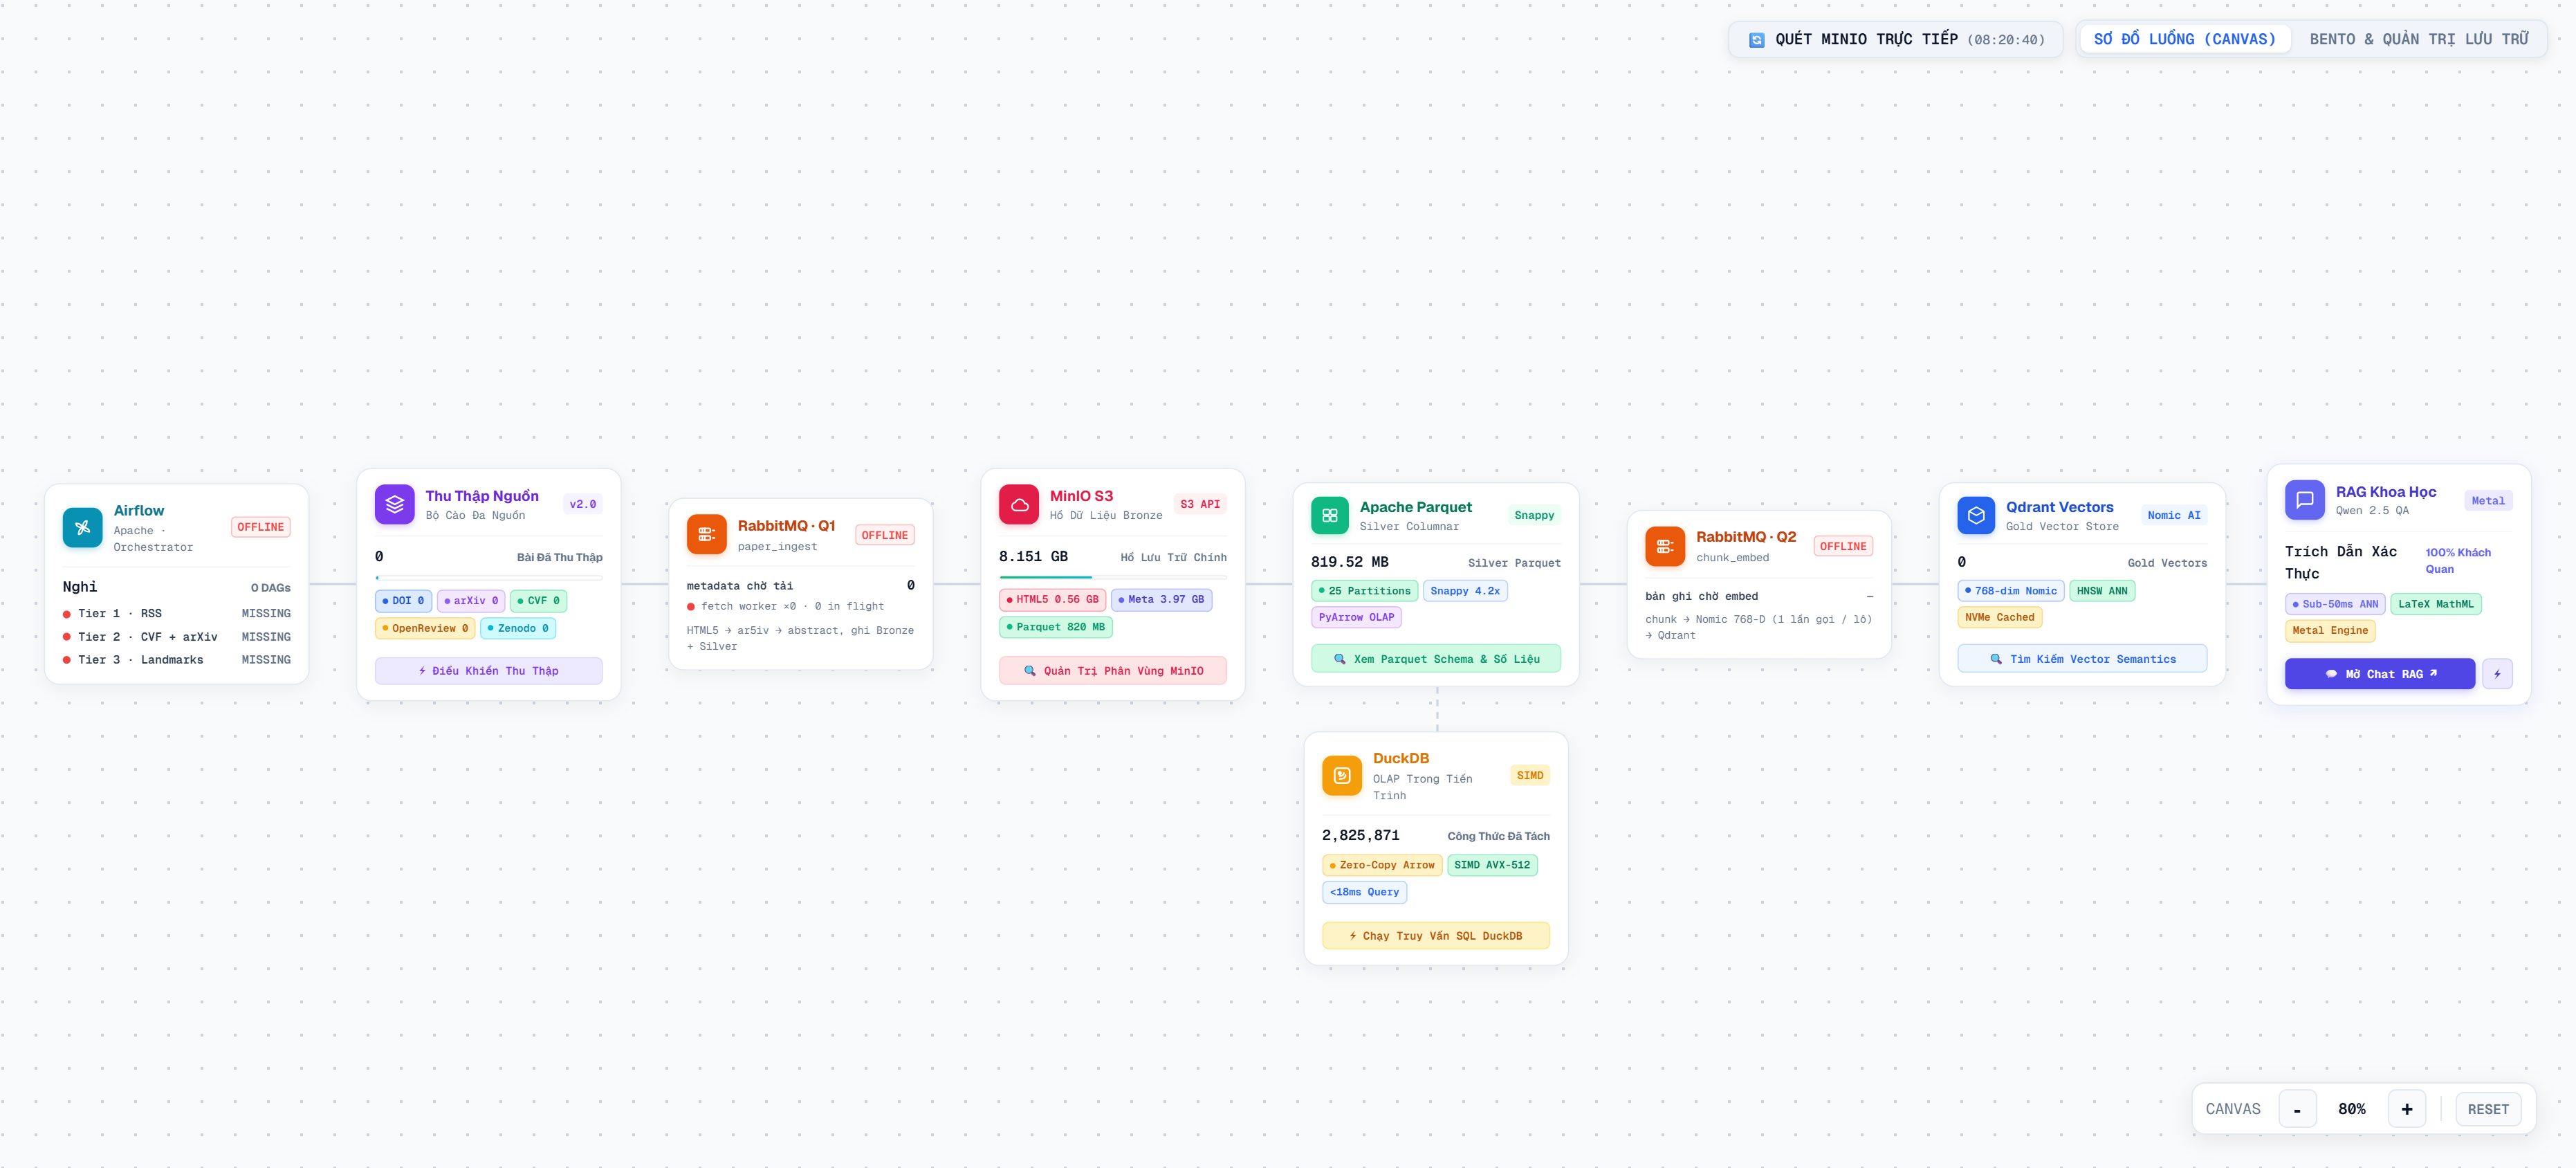
\includegraphics[width=\linewidth,height=0.68\textheight,keepaspectratio]{figures/captured_20261123_082337/01_pipeline_ui.png}
\caption[Giao diện giám sát luồng dữ liệu Pipeline]{Giao diện giám sát luồng dữ liệu Pipeline}
\label{fig:pipeline_capture}
\ReportNote{Nguồn: Giao diện giám sát luồng dữ liệu (Data Pipeline Monitor) trên bảng điều khiển quản trị hệ thống.}
\end{figure}
\FloatBarrier

\section{Bảo Mật và Phân Quyền Truy Cập (Zero Trust \& Role-Based Access)}

Để phục vụ chia sẻ tài nguyên cho sinh viên và đồng môn trong lớp học nghiên cứu và giới hạn quyền ghi, tài liệu triển khai mô tả cơ chế \textbf{Zero Trust Access} thông qua Cloudflare Tunnel:

Các chính sách sau là cấu hình hạ tầng được tài liệu hóa, chưa được kiểm thử live trong lần đối chiếu. Các hành vi từ chối ghi/xóa là kỳ vọng cần kiểm thử bằng tài khoản tương ứng. Cloudflare Tunnel không tự xác nhận đã bật đầy đủ chính sách Zero Trust Access.
\subsection{Phân quyền MinIO Object Storage}
\begin{itemize}
  \item \textbf{Tài khoản Quản trị (Admin)}: Toàn quyền ghi dữ liệu hồ, cập nhật Parquet và cấu hình bucket.
  \item \textbf{Tài khoản Sinh viên / Khách (\texttt{guest\_student})}: Được gán chính sách phân quyền nghiêm ngặt \lstinline{student_readonly} (chỉ cho phép các hành động \texttt{s3:ListBucket} và \texttt{s3:GetObject}). Sinh viên có thể duyệt cây thư mục và tải dữ liệu Parquet về phân tích nghiên cứu, nhưng mọi hành động tải lên, ghi đè hoặc xóa tài liệu theo chính sách phải bị từ chối với mã lỗi \texttt{AccessDenied}.
\end{itemize}

\subsection{Phân quyền Qdrant Vector Database}
\begin{itemize}
  \item \textbf{Admin Master Key}: Dành riêng cho Backend và Ingestion Consumer để tạo collection và nạp (upsert) vector.
  \item \textbf{Read-Only API Key (\texttt{uth\_guest\_readonly\_key\_...})}: Cung cấp cho sinh viên thực hiện các truy vấn tìm kiếm ngữ nghĩa (\texttt{search}, \texttt{scroll}, \texttt{get points}). Mọi yêu cầu ghi/xóa (\path{POST /points/delete}, \path{DELETE /collections}) theo phân quyền phải bị từ chối với mã lỗi \textbf{\texttt{403 Forbidden}}.
\end{itemize}

\section{Quy Trình Khởi Chạy và Kiểm Thử Hệ Thống (Deployment SOP)}

Hệ thống cung cấp quy trình khởi chạy chuẩn hóa thông qua kịch bản tự động hoặc từng phân hệ độc lập:

\begin{enumerate}[label=\textbf{Bước \arabic*.}]
  \item \textbf{Khởi động Hạ tầng Docker}:
  \begin{lstlisting}[language=bash]
# Run in the external infrastructure Compose directory
docker compose up -d minio qdrant rabbitmq
cd airflow && docker compose up -d
  \end{lstlisting}
  \item \textbf{Cấu hình Biến Môi trường}:
  Sao chép tệp cấu hình mẫu và điền các thông số kết nối:
  \begin{lstlisting}[language=bash]
Copy-Item .env_example .env
  \end{lstlisting}
  \item \textbf{Khởi chạy Workers Xử lý Hàng đợi (RabbitMQ Consumers)}:
  Mở 2 tiến trình worker nền độc lập:
  \begin{lstlisting}[language=bash]
# Worker 1: Fetch -> Bronze + Silver papers -> embed queue
python -m src.ingestion.queue_consumer --stage fetch

# Worker 2: Embed -> Silver chunks -> Qdrant
python -m src.ingestion.queue_consumer --stage embed
  \end{lstlisting}
  \item \textbf{Khởi chạy Mô hình Ngôn ngữ LLM Cục bộ}:
  \begin{lstlisting}[language=bash]
# Chay Qwen2.5-7B Instruct qua llama-server voi CUDA
.\llama-server.exe -m models\qwen2.5-7b-instruct-q4_k_m\qwen2.5-7b-instruct-q4_k_m.gguf --port 9001 --ctx-size 4096 -ngl -1
  \end{lstlisting}
  \item \textbf{Khởi chạy Backend FastAPI và Frontend React}:
  \begin{lstlisting}[language=bash]
# Backend
python -m uvicorn backend.app.main:app --host 0.0.0.0 --port 8000 --reload

# Frontend
cd frontend && npm run dev
  \end{lstlisting}
\end{enumerate}

\section{Kế Hoạch Giám Sát và Khắc Phục Sự Cố (Monitoring \& Operations)}

\begin{itemize}
\item \textbf{Health}: \path{/api/health} trả readiness từ retrieval và kiểm tra tồn tại Silver primary key, kèm version/timestamp. Endpoint này không kiểm tra toàn diện RabbitMQ/LLM và không tự lập lịch mỗi 30 giây. Telemetry và trạng thái các phân hệ được cung cấp riêng.
\item \textbf{Ngân sách}: \texttt{LAKEHOUSE\_BUDGET\_GB} mặc định 20 GB. DAG ước lượng MinIO, Qdrant và dữ liệu đang chờ, tính số bài còn chỗ; dừng khi hết ngân sách ước lượng. Code không có quy tắc dừng tại 90\% như mô tả cũ.
\item \textbf{Backpressure}: Fetch chờ khi embed queue đạt ngưỡng 500 mặc định; Tier 2 phát lô và chờ ingest queue giảm, đồng thời cập nhật ngân sách.
\item \textbf{Khôi phục}: ACK thủ công sau ghi bền vững, thử lại riêng từng stage và DLQ khi quá giới hạn. Cơ chế upsert theo ID và dedup giảm tác động redelivery; vẫn cần theo dõi DLQ và bài đã có Silver nhưng thiếu vector.
\item \textbf{Bảo trì}: \path{scripts/migrate_chunks_to_silver.py} hỗ trợ di chuyển payload cũ; \path{scripts/backfill_missing_papers.py} hỗ trợ bổ sung bài thiếu Qdrant, có dry-run. Cần xác định chế độ chunking và backup trước khi chạy migration thực tế.
\end{itemize}


Các thao tác vận hành trên tạo điều kiện để kiểm tra ba lớp: dữ liệu có đọc và hydrate được hay không, dịch vụ có hoàn thành tác vụ hay không, và kết quả có đạt tiêu chí chất lượng hay không. Chỉ khi các lớp này được đo trên cùng phiên bản mới có thể kết luận độ sẵn sàng của nguyên mẫu và đánh giá giá trị ứng dụng ở chương cuối.

\clearpage

% Chương 7: Kết luận, Đe dọa tính hợp lệ & Hướng phát triển (Conclusion)
\chapter{Kết Luận và Hướng Phát Triển (Conclusion \& Future Work)}
\label{chap:conclusion}
\section{Tổng Kết Kết Quả và Phạm Vi Xác Nhận}
Báo cáo xem xét ba câu hỏi đặt ra ở Chương~\ref{chap:business_understanding}: tổ chức dữ liệu, khả năng khai phá corpus và mức chứng cứ đánh giá RAG. Kết quả được phân biệt theo chức năng đã triển khai và hiệu quả đã đo:
\begin{enumerate}
\item \textbf{Tổ chức và cập nhật}: Source tại commit \texttt{e828310} triển khai hai stage fetch/embed, Bronze và Silver papers/chunks, chỉ mục Qdrant cùng API phục vụ. Việc giữ text trong Silver tạo đường đối chiếu từ vector tới nội dung. Snapshot 10,000 bài là nguồn thống kê lịch sử; lịch thu thập hằng ngày chưa chứng minh độ trễ cập nhật thời gian thực hoặc một cơ chế đối sánh với baseline cố định.
\item \textbf{Khai phá corpus}: Các artifact lịch sử cho thấy khả năng xuất luật, profile cụm, đồ thị và danh sách dị biệt. Snapshot 10,000 bài ghi 2,220,938 công thức được đếm; FP-Growth ghi 282 giao dịch và 22 luật; graph là mạng đồng tác giả. Đây là kết quả mô tả trên dữ liệu quan sát, không đủ xác nhận chất lượng cụm, vai trò landmark hoặc độ chính xác nhãn dị biệt.
\item \textbf{Truy xuất và hỏi đáp}: PageRank điều chỉnh điểm retrieval/fusion trước bước cross-encoder; luật là annotation, còn clustering và anomaly phục vụ khám phá corpus. Luật, clustering và anomaly chưa được đưa vào prompt như một lớp ngữ cảnh mining riêng. DeepEval lịch sử trên LanceDB ghi Contextual Precision tăng lên 0.860 nhưng Faithfulness chỉ đạt 0.699 và một số metric giảm. Chưa có ablation xác nhận tác động riêng của từng thành phần hoặc nguyên nhân hạn chế grounding; kiến trúc Qdrant/Silver chunks cần được đánh giá lại thống nhất.
\end{enumerate}

\section{Đóng Góp và Giá Trị Ứng Dụng}
Đóng góp của đồ án là kết nối xử lý tài liệu học thuật, khai phá nhiều góc nhìn và hỏi đáp có nguồn trong một nguyên mẫu có thể kiểm tra theo từng tầng dữ liệu. Hai stage tách công việc thu thập khỏi nhúng; Silver chunks tách vòng đời nội dung khỏi payload vector; dashboard cung cấp các đầu ra khai phá để người đọc khảo sát corpus. Những lựa chọn này tạo cơ sở cho thí nghiệm tiếp theo, chưa phải chứng cứ rằng hệ thống tiết kiệm một lượng thời gian cụ thể hoặc luôn trả lời đúng.

Mạch phân tích từ EDA tới thiết kế chỉ ra ba ưu tiên: giữ section và công thức vì tài liệu có cấu trúc không đồng đều; giới hạn suy luận xu hướng vì corpus lệch thời gian; và kiểm tra chất lượng nội dung cùng đồng bộ chỉ mục trước khi đánh giá hiệu quả RAG. Vì vậy, đánh giá quy mô lưu trữ cần đi cùng đánh giá chất lượng dữ liệu và chất lượng câu trả lời.

\section{Giới Hạn Còn Tồn Tại}
\begin{enumerate}
\item Corpus tập trung vào một số chuyên ngành và tháng công bố; các snapshot và cỡ mẫu khác nhau không tạo thành một thực nghiệm thống nhất. Nhãn làm giàu và số công thức chưa đo độ chính xác trích xuất.
\item Luật có ít giao dịch hỗ trợ, profile cụm cũ có lỗi, Silhouette thấp và nhãn dị biệt chưa có ground truth. Điểm PageRank đồng tác giả không thay thế đánh giá ảnh hưởng bài báo; khớp tên tác giả còn nguy cơ nhập nhằng.
\item Benchmark RAG có ít câu hỏi, số mẫu hợp lệ khác nhau theo metric và sử dụng LLM judge. Một số chỉ số giảm sau nâng cấp; các bất nhất trong case study và baseline hiệu năng cần raw trace để xác minh.
\item Phiên bản mới chưa được đo lại đồng thời về chất lượng, độ trễ hydrate và độ bền vận hành. Chứng cứ hiện có chưa xác nhận lợi ích riêng của query expansion, authority hoặc từng thuật toán mining đối với retrieval.
\end{enumerate}

\section{Hướng Phát Triển}
Ưu tiên trước hết là tái lập một vòng đánh giá trên cùng commit, snapshot, model và cấu hình: kiểm tra dữ liệu đầu vào, tính nhất quán Silver/Qdrant, lưu raw traces và công bố số mẫu lỗi. Kiểm tra thủ công một mẫu công thức cùng nhãn dị biệt để bổ sung đánh giá chất lượng ngoài số lượng đầu ra.

Tiếp theo, thực hiện ablation giữa dense retrieval, lexical/RRF, authority và reranker; nếu triển khai query expansion thực sự thì đánh giá riêng độ phủ và nhiễu truy xuất. Cụm cần được diễn giải bằng tài liệu đại diện và kiểm tra độ ổn định theo $K$; phân tích tương quan cần xác nhận mẫu và xử lý nhiều phép so sánh. Khi dữ liệu citation cùng phép đo nền đã đủ tin cậy, mới mở rộng graph tri thức, multi-hop RAG và nghiên cứu người dùng.

\clearpage

% --- PHẦN CUỐI (BACK MATTER) ---
% Danh mục Tài liệu tham khảo chuẩn BibTeX
\bibliographystyle{ieeetr}
\bibliography{references}
\clearpage

% Phụ lục (Appendix): Ma trận đối chiếu, Mã nguồn mẫu, Hướng dẫn cài đặt
% ==============================================================================
% PHỤ LỤC (APPENDIX)
% ==============================================================================

\chapter*{PHỤ LỤC}
\addcontentsline{toc}{chapter}{Phụ lục}
\renewcommand{\thesection}{\Alph{section}}
\renewcommand{\theHsection}{appendix.\Alph{section}}
\setcounter{section}{0}
\counterwithin{figure}{section}
\renewcommand{\theHfigure}{appendix.\thesection.\arabic{figure}}
\counterwithout{lstlisting}{chapter}
\counterwithin{lstlisting}{section}

\section{Đối Chiếu Nguồn Gốc Báo Cáo và Mã Nguồn Thực Tế (Traceability Overview)}

Nhằm bảo đảm tính minh bạch học thuật, bản cập nhật phân biệt implementation hiện tại, artifact local lịch sử và benchmark được tài liệu hóa; các nguồn tương ứng được liệt kê dưới đây:

\begin{itemize}[leftmargin=1.5cm]
  \item \textbf{Chương 1 (Hiểu bài toán \& KPI)}: \path{docs/OVERVIEW.md}, \path{SETUP.md}.
  \item \textbf{Chương 2 (Khám phá EDA \& Thống kê)}: \path{data/gold/mining/eda_summary.json}, \path{src/mining/eda_engine.py}.
  \item \textbf{Chương 3 (Thu thập 3 tầng \& Lakehouse)}: \path{src/ingestion/arxiv_batch_harvester.py}, \path{src/storage/duckdb_engine.py}, \path{src/transformation/html_parser.py}, \path{src/indexing/qdrant_manager.py}.
  \item \textbf{Chương 4 (4 Trụ cột Khai phá Dữ liệu \& RAG)}: \path{src/mining/association_rules.py}, \path{src/mining/cluster_analysis.py}, \path{src/mining/graph_mining.py}, \path{src/mining/trend_anomaly_mining.py}, \path{backend/app/services/retrieval_service.py}.
  \item \textbf{Chương 5 (Đánh giá DeepEval \& Hiệu năng GPU)}: \path{docs/benchmarks/RAG_EVALUATION_REPORT_21_SAMPLES.md}, \path{docs/benchmarks/PERFORMANCE_BENCHMARK_REPORT.md}.
  \item \textbf{Chương 6 (Triển khai Vận hành)}: \path{README.md}, \path{.env_example}, \path{dags/}, \path{backend/app/main.py}.
\end{itemize}

\subsection{Mốc Đối Chiếu và Tính Tái Lập}
Quy ước của báo cáo: source xác nhận đường xử lý đã triển khai; artifact ghi đầu ra của một snapshot; benchmark ghi kết quả của một phép đo; ảnh giao diện minh họa cách hiển thị. Chứng cứ thuộc loại này không tự thay thế loại khác. Các phép tính bổ sung như số giao dịch hỗ trợ, tổng thời gian hoặc tỷ số đều được suy từ số đã lưu và ghi rõ giới hạn làm tròn; không có lần chạy mining/benchmark mới.

Mã nguồn: commit \texttt{f421707}, ngày 09/11/2026; ngày cập nhật báo cáo 25/11/2026. Không chạy lại mining hoặc benchmark; frontend/backend không bị sửa đổi. Các file JSON local được xem là snapshot lịch sử; manifest tham chiếu ngày 04/10/2026 không xác nhận mọi artifact đã được tái lập cùng một lần chạy.

DeepEval: report 05/10/2026 ghi commit \texttt{6cb1c52}, LanceDB, hơn 143 nghìn chunk. Hiệu năng phần cứng: report 19/10/2026. Các benchmark bổ sung giai đoạn 06--08/11/2026 nằm tại \path{logs/benchmarks/} (\path{chunking_ab/summary.json}, \path{rag_eval/report_retrieval.json}) và \path{notebooks/} (\path{laya_onnx_20261108-2053_seed0/RUN_INFO.json}, \path{laya_finetune/report_seed0.json}). Các số quy mô citation và landmark chưa có artifact đối chiếu được loại khỏi bảng kết quả.

\subsection{Nguồn Bổ Sung cho Kiến Trúc Mới}
\begin{itemize}
\item \path{src/storage/chunk_store.py}, \path{src/indexing/qdrant_manager.py}: schema chunk, payload tối thiểu, hydrate và compaction.
\item \path{src/ingestion/queue_consumer.py}, \path{dags/dag_tier1_realtime_stream.py}, \path{dags/dag_tier2_near_past_harvest.py}, \path{dags/dag_compact_silver.py}: hai stage, lịch và backpressure.
\item \path{src/utils/hasher.py}, \path{src/storage/known_papers.py}, \path{src/transformation/silver_writer.py}: abstract hash và dedup.
\item \path{backend/app/core/config.py}, \path{backend/app/schemas/chat.py}, \path{backend/app/services/rag_service.py}: mặc định reranker/chat.
\item \path{benchmarks/rag_eval/}, \path{benchmarks/laya_finetune/}, \path{benchmarks/chunking_ab/}: bộ đánh giá Retrieval v1, fine-tune Laya ONNX và Chunking A/B.
\end{itemize}

\subsection{Bộ Ảnh Chụp Tự Động Ngày 23/11/2026}
Bộ ảnh gồm Pipeline, metadata Bronze, EDA Silver, hai ma trận tương quan, GMM và manifest Gold. PNG gốc, nguồn API, thời điểm chụp và SHA-256 nằm trong \path{figures/captured_20261123_082337/manifest.json}; các response dùng đối chiếu nằm trong thư mục \path{evidence/} cùng bộ ảnh.

Hình~\ref{fig:gold_manifest_capture} hiển thị cấu trúc tệp manifest định danh các sản phẩm khai phá dữ liệu thuộc tầng Gold, lưu trữ các siêu dữ liệu cấu hình và đường dẫn artifact phục vụ việc truy xuất và tái lập kết quả.
\begin{figure}[!htbp]
\centering
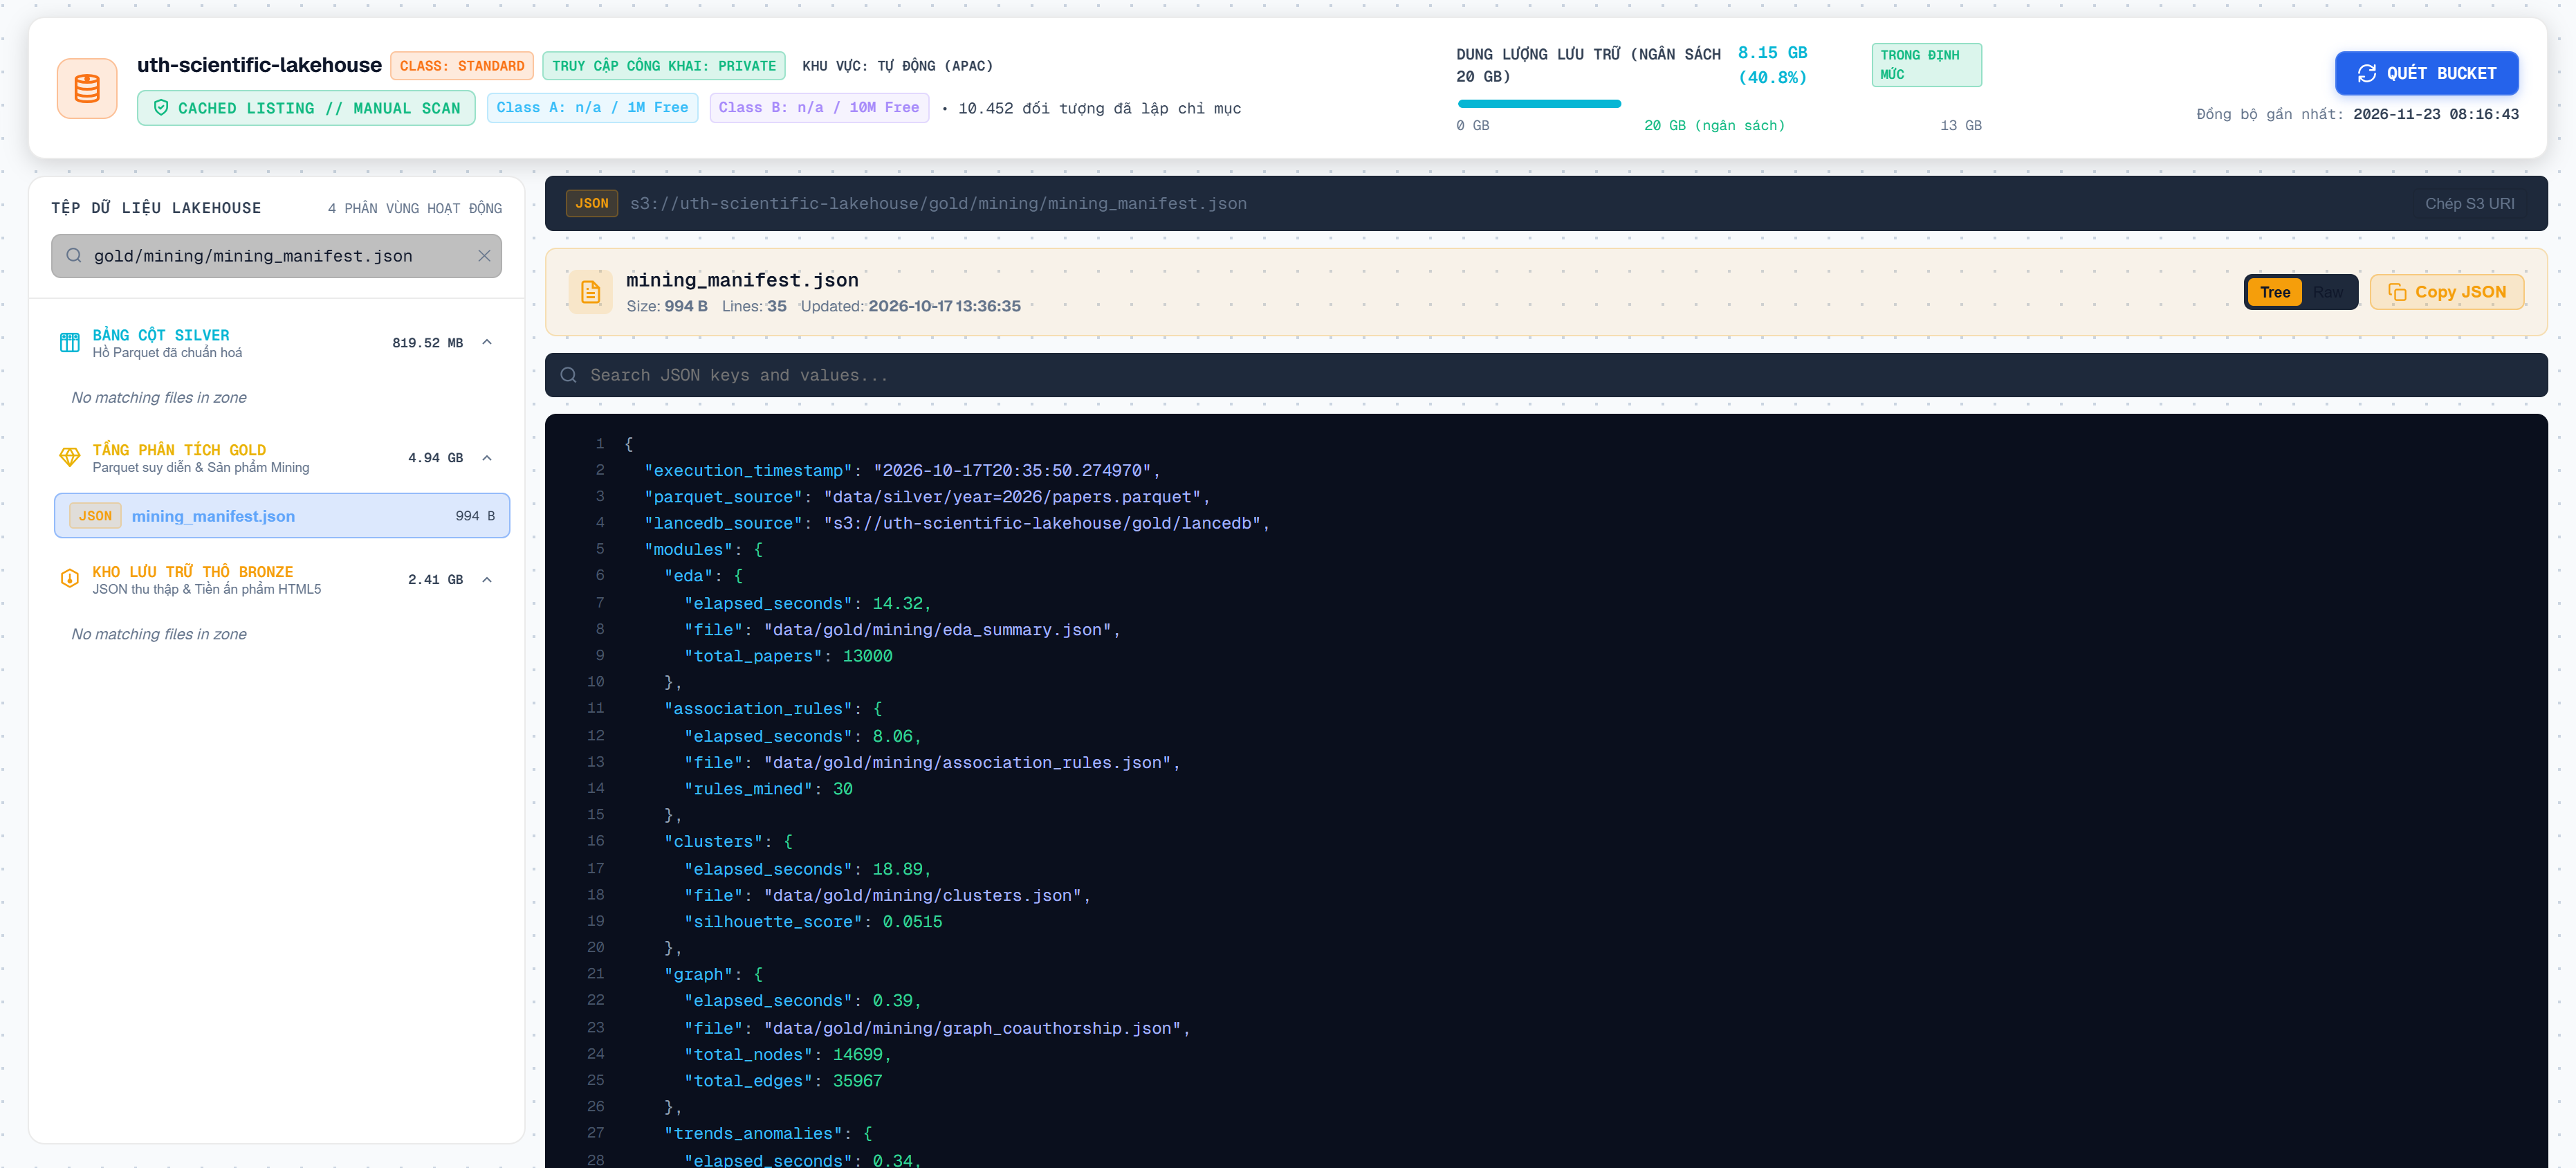
\includegraphics[width=\linewidth,height=0.68\textheight,keepaspectratio]{figures/captured_20261123_082337/07_gold_mining_manifest.png}
\caption[Manifest của các sản phẩm khai phá Gold]{Manifest của các sản phẩm khai phá Gold}
\label{fig:gold_manifest_capture}
\ReportNote{Nguồn: Tệp kê khai định danh và thông số các sản phẩm khai phá dữ liệu tầng Gold (\path{gold/mining/mining_manifest.json}).}
\end{figure}
\FloatBarrier

\section{Trích Đoạn Mã Nguồn Tiêu Biểu (Key Code Listings)}

\subsection{Thuật toán Khai phá Luật Kết hợp FP-Growth với Khử Trùng lặp Đối xứng}
Đoạn mã trích từ \path{src/mining/association_rules.py} thể hiện quá trình một-nóng hóa giao dịch, dựng cây FP-Tree và lọc luật đối xứng theo giá trị Lift và Confidence:

\begin{lstlisting}[language=Python, caption={Khử trùng lặp luật đối xứng trong AssociationRuleMiner}]
# Trich doan tu src/mining/association_rules.py
te = TransactionEncoder()
te_ary = te.fit_transform(transactions)
df_encoded = pd.DataFrame(te_ary, columns=te.columns_)

# Khai pha tap muc pho bien bang FP-Growth
frequent_itemsets = fpgrowth(df_encoded, min_support=min_support, use_colnames=True)

# Sinh luat ket hop theo do nang Lift
rules = association_rules(frequent_itemsets, metric="lift", min_threshold=min_lift)
rules = rules.assign(_lift_key=rules["lift"].round(6))
sorted_rules = rules.sort_values(by=["_lift_key", "confidence"], ascending=[False, False])

# Khu trung lap luat doi xung: giu lai chieu co Confidence cao hon
deduped_rows = []
seen_pairs = set()
for _, row in sorted_rules.iterrows():
    ant = tuple(sorted(list(row["antecedents"])))
    con = tuple(sorted(list(row["consequents"])))
    pair_key = frozenset([ant, con])
    if pair_key in seen_pairs:
        continue
    seen_pairs.add(pair_key)
    deduped_rows.append(row)
\end{lstlisting}

\subsection{Cơ chế Tăng cường Điểm Uy tín PageRank trong Thuật toán Tìm kiếm Lai (RAG Retrieval)}
Đoạn mã trích từ \path{backend/app/services/retrieval_service.py} thể hiện việc ánh xạ tác giả bài báo với các nút có điểm PageRank cao trong artifact graph được nạp (citation hoặc đồng tác giả):

\begin{lstlisting}[language=Python, caption={Bộ nhân uy tín PageRank Authority Multiplier}]
# Trich doan tu backend/app/services/retrieval_service.py
def _match_authority(self, authors: List[str]) -> Tuple[float, Optional[str]]:
    """Anh xa tac gia cua doan trich voi cac nut co PageRank cao trong mang luoi."""
    self._ensure_graph_and_rules()
    if not authors or not self.influencers:
        return 0.0, None

    best_pr = 0.0
    best_author = None
    for a in authors:
        a_lower = a.lower().strip()
        for inf in self.influencers:
            if inf["author_clean"] in a_lower or a_lower in inf["author_clean"]:
                if inf["pagerank"] > best_pr:
                    best_pr = inf["pagerank"]
                    best_author = a

    if best_pr > 0.0:
        norm_pr = min(1.0, best_pr / max(1e-6, self.max_pagerank))
        return norm_pr, best_author
    return 0.0, None
\end{lstlisting}

\Needspace{9\baselineskip}
\subsection{Phát hiện Bài báo Dị biệt Cấu trúc Bằng Rừng Cô Lập với Chuẩn hóa $\log(1+x)$}
Đoạn mã trích từ \path{src/mining/trend_anomaly_mining.py}:

\begin{lstlisting}[language=Python, caption={Isolation Forest tren dac trung log1p}]
# Trich doan tu src/mining/trend_anomaly_mining.py
feature_cols = [
    "total_math_count",
    "total_words",
    "total_sections",
    "author_count",
    "category_count",
]
X_raw = df[feature_cols].fillna(0).values.astype(np.float64)
# Chuan hoa log(1+x) de giam do lech phan phoi duoi dai
X_log = np.log1p(X_raw)

iso_forest = IsolationForest(
    contamination=contamination,
    random_state=42,
    n_estimators=100,
)
preds = iso_forest.fit_predict(X_log)
anomaly_scores = iso_forest.score_samples(X_log)
df["is_anomaly"] = preds == -1
\end{lstlisting}


\subsection{Payload Vector Tối Thiểu và Hydrate từ Silver}
Đoạn mã được trích từ \path{src/storage/chunk_store.py} và \path{src/indexing/qdrant_manager.py}, đối chiếu tới commit \texttt{f421707}. Qdrant giữ trường định danh/lọc; kết quả thiếu text được bổ sung từ bảng chunk Silver. Các dấu ngắt dưới đây phân tách các đoạn trích từ hai module, không biểu diễn một script độc lập.
\lstinputlisting[language=Python,caption={Trường payload và hydrate nội dung từ Silver},label={lst:payload_hydrate}]{listings/qdrant_payload_hydrate.py}

\subsection{Ghi Silver Chunks Trước Khi Upsert Vector}
Đoạn trích từ \path{src/ingestion/queue_consumer.py}, đối chiếu tới commit \texttt{f421707}, cho thấy thứ tự ghi chunk table và nhánh bỏ qua các bài thuộc phân vùng ghi thất bại. Chỉ các đoạn liên quan được giữ; vị trí lược bớt được đánh dấu bằng chú thích.
\lstinputlisting[language=Python,caption={Thứ tự ghi Silver chunks và upsert Qdrant},label={lst:silver_before_vector}]{listings/silver_before_vector.py}

\Needspace{12\baselineskip}
\section{Hướng Dẫn Cài Đặt và Khởi Chạy Nhanh Dự Án}

\subsection{Cài đặt môi trường Python}
\begin{lstlisting}[language=bash]
# 1. Tao moi truong ao
python -m venv .venv

# 2. Kich hoat moi truong ao (Windows PowerShell)
.\.venv\Scripts\Activate.ps1

# 3. Cai dat cac goi thu vien phu thuoc
pip install --upgrade pip
pip install -r requirements.txt
pip install -e .
\end{lstlisting}

\subsection{Các lệnh kiểm thử tham khảo}
\begin{lstlisting}[language=bash]
# Unit tests; integration tests require configured external services
pytest tests/unit/ -v
pytest tests/integration/ -v
\end{lstlisting}


\end{document}
